\documentclass{article}\usepackage[]{graphicx}\usepackage[]{color}
%% maxwidth is the original width if it is less than linewidth
%% otherwise use linewidth (to make sure the graphics do not exceed the margin)
\makeatletter
\def\maxwidth{ %
  \ifdim\Gin@nat@width>\linewidth
    \linewidth
  \else
    \Gin@nat@width
  \fi
}
\makeatother

\definecolor{fgcolor}{rgb}{0.345, 0.345, 0.345}
\newcommand{\hlnum}[1]{\textcolor[rgb]{0.686,0.059,0.569}{#1}}%
\newcommand{\hlstr}[1]{\textcolor[rgb]{0.192,0.494,0.8}{#1}}%
\newcommand{\hlcom}[1]{\textcolor[rgb]{0.678,0.584,0.686}{\textit{#1}}}%
\newcommand{\hlopt}[1]{\textcolor[rgb]{0,0,0}{#1}}%
\newcommand{\hlstd}[1]{\textcolor[rgb]{0.345,0.345,0.345}{#1}}%
\newcommand{\hlkwa}[1]{\textcolor[rgb]{0.161,0.373,0.58}{\textbf{#1}}}%
\newcommand{\hlkwb}[1]{\textcolor[rgb]{0.69,0.353,0.396}{#1}}%
\newcommand{\hlkwc}[1]{\textcolor[rgb]{0.333,0.667,0.333}{#1}}%
\newcommand{\hlkwd}[1]{\textcolor[rgb]{0.737,0.353,0.396}{\textbf{#1}}}%

\usepackage{framed}
\makeatletter
\newenvironment{kframe}{%
 \def\at@end@of@kframe{}%
 \ifinner\ifhmode%
  \def\at@end@of@kframe{\end{minipage}}%
  \begin{minipage}{\columnwidth}%
 \fi\fi%
 \def\FrameCommand##1{\hskip\@totalleftmargin \hskip-\fboxsep
 \colorbox{shadecolor}{##1}\hskip-\fboxsep
     % There is no \\@totalrightmargin, so:
     \hskip-\linewidth \hskip-\@totalleftmargin \hskip\columnwidth}%
 \MakeFramed {\advance\hsize-\width
   \@totalleftmargin\z@ \linewidth\hsize
   \@setminipage}}%
 {\par\unskip\endMakeFramed%
 \at@end@of@kframe}
\makeatother

\definecolor{shadecolor}{rgb}{.97, .97, .97}
\definecolor{messagecolor}{rgb}{0, 0, 0}
\definecolor{warningcolor}{rgb}{1, 0, 1}
\definecolor{errorcolor}{rgb}{1, 0, 0}
\newenvironment{knitrout}{}{} % an empty environment to be redefined in TeX

\usepackage{alltt}
\usepackage{geometry}
\usepackage{amsmath}
\usepackage{lscape}
\geometry{verbose,tmargin=2.5cm,bmargin=2.5cm,lmargin=2.5cm,rmargin=2.5cm}
\IfFileExists{upquote.sty}{\usepackage{upquote}}{}
\begin{document}



\title{NSWPCN Predictor Training}
\maketitle

%%%%%%%%%%%%%%%%%%%%%%%%%%%%%%%%%%%%%%%%%%%%%%%%%%%%%%%%%%%%%%%%%%%%%%
% LIBRARIES
%%%%%%%%%%%%%%%%%%%%%%%%%%%%%%%%%%%%%%%%%%%%%%%%%%%%%%%%%%%%%%%%%%%%%%
\section{Preparation}
\begin{knitrout}
\definecolor{shadecolor}{rgb}{0.969, 0.969, 0.969}\color{fgcolor}\begin{kframe}
\begin{alltt}
\hlkwd{library}\hlstd{(survival)}
\end{alltt}


{\ttfamily\noindent\itshape\color{messagecolor}{\#\# Loading required package: splines}}\begin{alltt}
\hlkwd{library}\hlstd{(glmulti)}
\end{alltt}


{\ttfamily\noindent\itshape\color{messagecolor}{\#\# Loading required package: rJava\\\#\# Loading required package: methods}}\begin{alltt}
\hlkwd{library}\hlstd{(flexsurv)}
\hlkwd{library}\hlstd{(randomForestSRC)}
\end{alltt}


{\ttfamily\noindent\itshape\color{messagecolor}{\#\# Loading required package: parallel\\\#\# \\\#\#\ \ randomForestSRC 1.5.5 \\\#\#\ \ \\\#\#\ \ Type rfsrc.news() to see new features, changes, and bug fixes. \\\#\# }}\begin{alltt}
\hlkwd{library}\hlstd{(reshape2)}
\hlkwd{library}\hlstd{(plyr)}
\hlkwd{library}\hlstd{(ggplot2)}

\hlkwd{library}\hlstd{(MASS)}

\hlkwd{load}\hlstd{(}\hlstr{"03_NSWPCN_subset.rda"}\hlstd{)}
\end{alltt}
\end{kframe}
\end{knitrout}


%%%%%%%%%%%%%%%%%%%%%%%%%%%%%%%%%%%%%%%%%%%%%%%%%%%%%%%%%%%%%%%%%%%%%%
% DATA SELECTION
%%%%%%%%%%%%%%%%%%%%%%%%%%%%%%%%%%%%%%%%%%%%%%%%%%%%%%%%%%%%%%%%%%%%%%
\section{Cohort selection and transformation}
\begin{knitrout}
\definecolor{shadecolor}{rgb}{0.969, 0.969, 0.969}\color{fgcolor}\begin{kframe}
\begin{alltt}
\hlstd{x} \hlkwb{=} \hlstd{data[,} \hlkwd{c}\hlstd{(}\hlstr{"Patient.Sex"}\hlstd{,} \hlstr{"History.Diagnosis.AgeAt.Cent"}\hlstd{,} \hlstr{"Path.LocationBody"}\hlstd{,}
    \hlstr{"Path.Size.Cent"}\hlstd{,} \hlstr{"Path.Ca199.Preop"}\hlstd{,} \hlstr{"Molec.S100A2.DCThresh"}\hlstd{,} \hlstr{"Molec.S100A4.DCThresh"}\hlstd{)]}
\hlkwd{colnames}\hlstd{(x)} \hlkwb{=} \hlkwd{c}\hlstd{(}\hlstr{"SexM"}\hlstd{,} \hlstr{"AgeCent"}\hlstd{,} \hlstr{"LocBody"}\hlstd{,} \hlstr{"SizeCent"}\hlstd{,} \hlstr{"Ca199"}\hlstd{,} \hlstr{"A2"}\hlstd{,} \hlstr{"A4"}\hlstd{)}
\hlstd{x}\hlopt{$}\hlstd{SexM} \hlkwb{=} \hlstd{x}\hlopt{$}\hlstd{Sex} \hlopt{==} \hlstr{"M"}
\hlstd{x}\hlopt{$}\hlstd{Ca199} \hlkwb{=} \hlstd{x}\hlopt{$}\hlstd{Ca199} \hlopt{>} \hlnum{100}

\hlstd{y} \hlkwb{=} \hlkwd{Surv}\hlstd{(}\hlkwd{as.numeric}\hlstd{(data}\hlopt{$}\hlstd{History.Death.Date} \hlopt{-} \hlstd{data}\hlopt{$}\hlstd{History.Diagnosis.Date),}
    \hlstd{data}\hlopt{$}\hlstd{History.DSDeath.Event)}
\hlcom{# Note no surgery dates, though for almost all pts there were only a few}
\hlcom{# days difference.}

\hlstd{temp} \hlkwb{=} \hlnum{NA}
\hlstd{temp} \hlkwb{=} \hlkwd{ls}\hlstd{()}
\hlkwd{rm}\hlstd{(}\hlkwc{list} \hlstd{= temp[}\hlopt{!}\hlstd{(temp} \hlopt \hlkwd{c}\hlstd{(}\hlstr{"x"}\hlstd{,} \hlstr{"y"}\hlstd{))])}

\hlstd{sel} \hlkwb{=} \hlopt{!}\hlkwd{is.na}\hlstd{(y[,} \hlnum{1}\hlstd{])} \hlopt{& !}\hlkwd{is.na}\hlstd{(y[,} \hlnum{2}\hlstd{])} \hlopt{& !}\hlkwd{is.na}\hlstd{(x}\hlopt{$}\hlstd{A2)} \hlopt{& !}\hlkwd{is.na}\hlstd{(x}\hlopt{$}\hlstd{A4)} \hlopt{& !}\hlkwd{is.na}\hlstd{(x}\hlopt{$}\hlstd{LocBody)}
\hlstd{x} \hlkwb{=} \hlstd{x[sel, ]}
\hlstd{y} \hlkwb{=} \hlstd{y[sel, ]}
\hlkwd{rm}\hlstd{(sel)}

\hlcom{# Remove CA-19-9 measurements as they're mostly missing}
\hlstd{x} \hlkwb{=} \hlstd{x[,} \hlkwd{colnames}\hlstd{(x)} \hlopt{!=} \hlstr{"Ca199"}\hlstd{]}

\hlstd{data} \hlkwb{=} \hlkwd{as.data.frame}\hlstd{(}\hlkwd{cbind}\hlstd{(}\hlkwc{Time} \hlstd{= y[,} \hlnum{1}\hlstd{],} \hlkwc{DSD} \hlstd{= y[,} \hlnum{2}\hlstd{], x))}
\hlkwd{rm}\hlstd{(x, y)}
\hlstd{data}\hlopt{$}\hlstd{DSD} \hlkwb{=} \hlstd{data}\hlopt{$}\hlstd{DSD} \hlopt{==} \hlnum{1}
\end{alltt}
\end{kframe}
\end{knitrout}


%%%%%%%%%%%%%%%%%%%%%%%%%%%%%%%%%%%%%%%%%%%%%%%%%%%%%%%%%%%%%%%%%%%%%%
% DATA SPLITTING
%%%%%%%%%%%%%%%%%%%%%%%%%%%%%%%%%%%%%%%%%%%%%%%%%%%%%%%%%%%%%%%%%%%%%%
\section{Data splitting}
There's going to be an awful lot of model manipulation and black magic going on.  Create a holdout validation set for final model comparison and selection.
\begin{knitrout}
\definecolor{shadecolor}{rgb}{0.969, 0.969, 0.969}\color{fgcolor}\begin{kframe}
\begin{alltt}
\hlkwd{set.seed}\hlstd{(}\hlnum{20150110}\hlstd{)}
\hlstd{sel.val} \hlkwb{=} \hlkwd{sample.int}\hlstd{(}\hlkwd{nrow}\hlstd{(data),} \hlkwd{floor}\hlstd{(}\hlkwd{nrow}\hlstd{(data)}\hlopt{/}\hlnum{5}\hlstd{))}
\hlstd{sel.val} \hlkwb{=} \hlnum{1}\hlopt{:}\hlkwd{nrow}\hlstd{(data)} \hlopt \hlstd{sel.val}
\hlkwd{mean}\hlstd{(sel.val)}
\end{alltt}
\begin{verbatim}
## [1] 0.1967
\end{verbatim}
\begin{alltt}
\hlstd{data.val} \hlkwb{=} \hlstd{data[sel.val, ,} \hlkwc{drop} \hlstd{=} \hlnum{FALSE}\hlstd{]}
\hlstd{data} \hlkwb{=} \hlstd{data[}\hlopt{!}\hlstd{sel.val, ,} \hlkwc{drop} \hlstd{=} \hlnum{FALSE}\hlstd{]}
\end{alltt}
\end{kframe}
\end{knitrout}


%%%%%%%%%%%%%%%%%%%%%%%%%%%%%%%%%%%%%%%%%%%%%%%%%%%%%%%%%%%%%%%%%%%%%%
% MODEL SPECIFICATION
%%%%%%%%%%%%%%%%%%%%%%%%%%%%%%%%%%%%%%%%%%%%%%%%%%%%%%%%%%%%%%%%%%%%%%
\section{EDA}
Use the CPH model as a convenient framework for EDA.
\subsection{Functional form}
Investigate functional form with martingale residuals.
\begin{knitrout}
\definecolor{shadecolor}{rgb}{0.969, 0.969, 0.969}\color{fgcolor}\begin{kframe}
\begin{alltt}
\hlstd{fit.cph.NoAge} \hlkwb{=} \hlkwd{coxph}\hlstd{(}\hlkwd{Surv}\hlstd{(Time, DSD)} \hlopt{~} \hlstd{SexM} \hlopt{+} \hlstd{LocBody} \hlopt{+} \hlstd{SizeCent} \hlopt{+} \hlstd{A2} \hlopt{+} \hlstd{A4,}
    \hlkwc{data} \hlstd{= data)}
\hlstd{fit.cph.NoSize} \hlkwb{=} \hlkwd{coxph}\hlstd{(}\hlkwd{Surv}\hlstd{(Time, DSD)} \hlopt{~} \hlstd{SexM} \hlopt{+} \hlstd{AgeCent} \hlopt{+} \hlstd{LocBody} \hlopt{+} \hlstd{A2} \hlopt{+} \hlstd{A4,}
    \hlkwc{data} \hlstd{= data)}
\hlkwd{scatter.smooth}\hlstd{(data}\hlopt{$}\hlstd{AgeCent,} \hlkwd{resid}\hlstd{(fit.cph.NoAge,} \hlkwc{type} \hlstd{=} \hlstr{"martingale"}\hlstd{),} \hlkwc{main} \hlstd{=} \hlstr{"Functional form: Age (Centered)"}\hlstd{,}
    \hlkwc{xlab} \hlstd{=} \hlstr{"AgeCent"}\hlstd{,} \hlkwc{ylab} \hlstd{=} \hlstr{"Martingale residual"}\hlstd{)}
\end{alltt}
\end{kframe}

{\centering 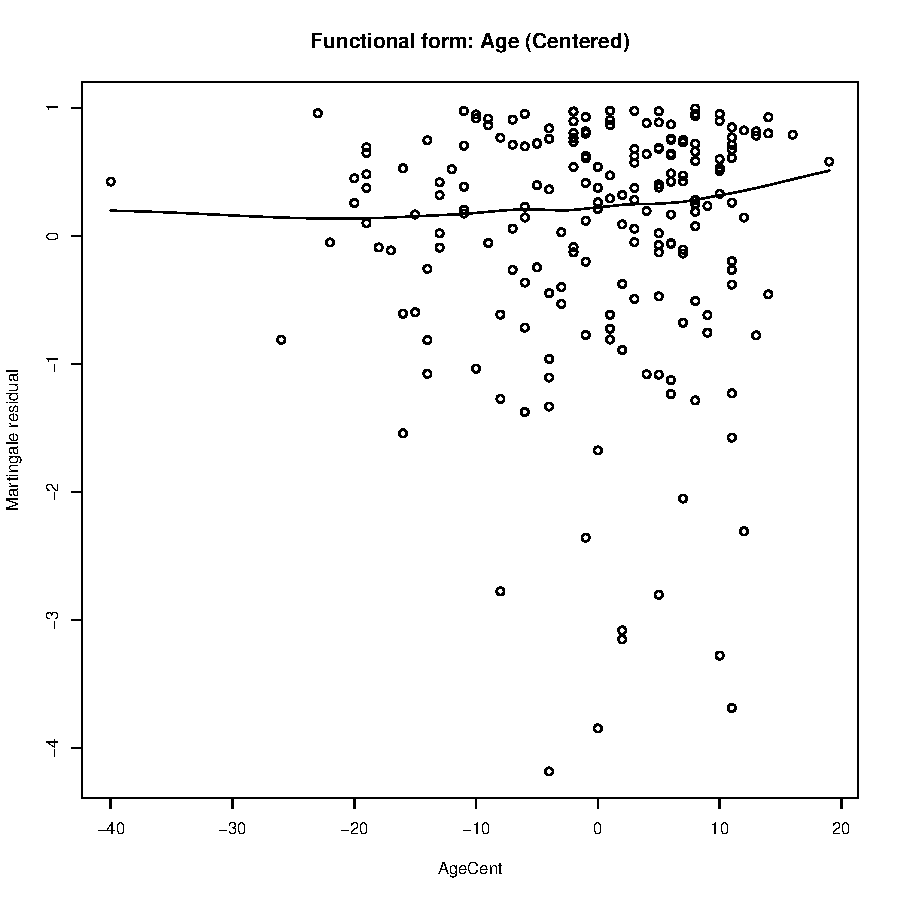
\includegraphics[width=\maxwidth]{figure/eda-func-form-1} 

}


\begin{kframe}\begin{alltt}
\hlkwd{scatter.smooth}\hlstd{(data}\hlopt{$}\hlstd{AgeCent,} \hlkwd{resid}\hlstd{(fit.cph.NoAge,} \hlkwc{type} \hlstd{=} \hlstr{"martingale"}\hlstd{),} \hlkwc{main} \hlstd{=} \hlstr{"Functional form: Age (Centered)"}\hlstd{,}
    \hlkwc{xlab} \hlstd{=} \hlstr{"AgeCent"}\hlstd{,} \hlkwc{ylab} \hlstd{=} \hlstr{"Martingale residual"}\hlstd{,} \hlkwc{ylim} \hlstd{=} \hlkwd{c}\hlstd{(}\hlopt{-}\hlnum{1}\hlstd{,} \hlnum{1}\hlstd{))}
\end{alltt}
\end{kframe}

{\centering 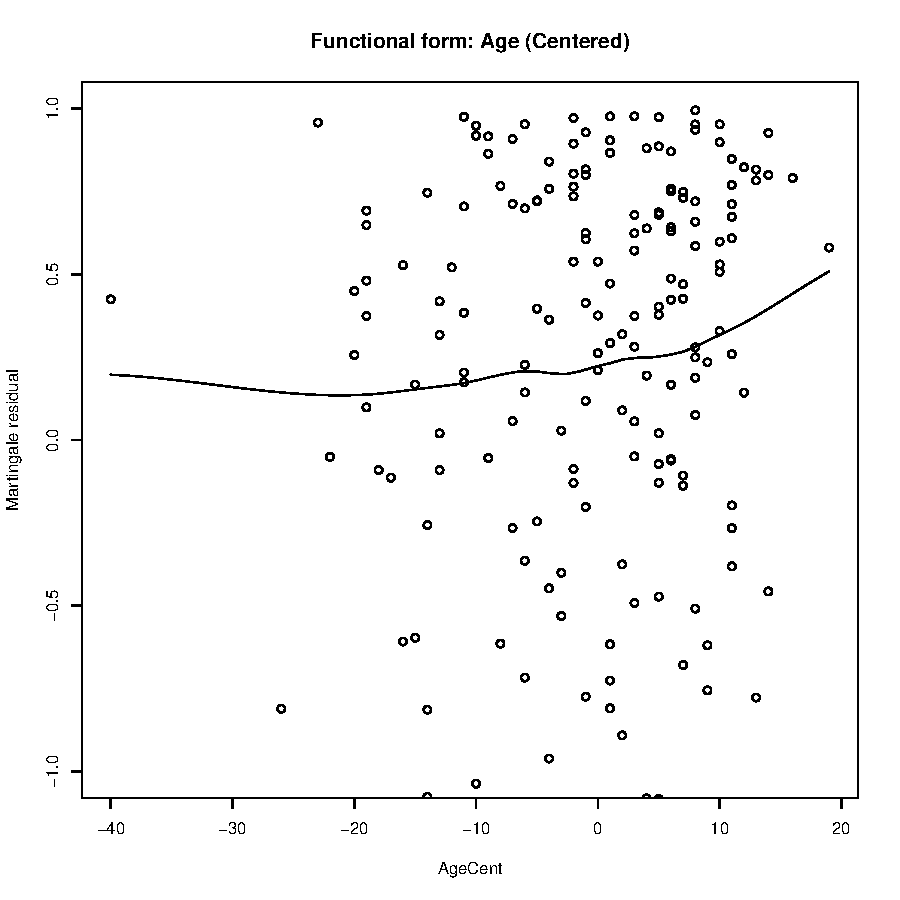
\includegraphics[width=\maxwidth]{figure/eda-func-form-2} 

}


\begin{kframe}\begin{alltt}
\hlkwd{scatter.smooth}\hlstd{(data}\hlopt{$}\hlstd{SizeCent,} \hlkwd{resid}\hlstd{(fit.cph.NoSize,} \hlkwc{type} \hlstd{=} \hlstr{"martingale"}\hlstd{),} \hlkwc{main} \hlstd{=} \hlstr{"Functional form: Size (Centered)"}\hlstd{,}
    \hlkwc{xlab} \hlstd{=} \hlstr{"SizeCent"}\hlstd{,} \hlkwc{ylab} \hlstd{=} \hlstr{"Martingale residual"}\hlstd{)}
\end{alltt}
\end{kframe}

{\centering 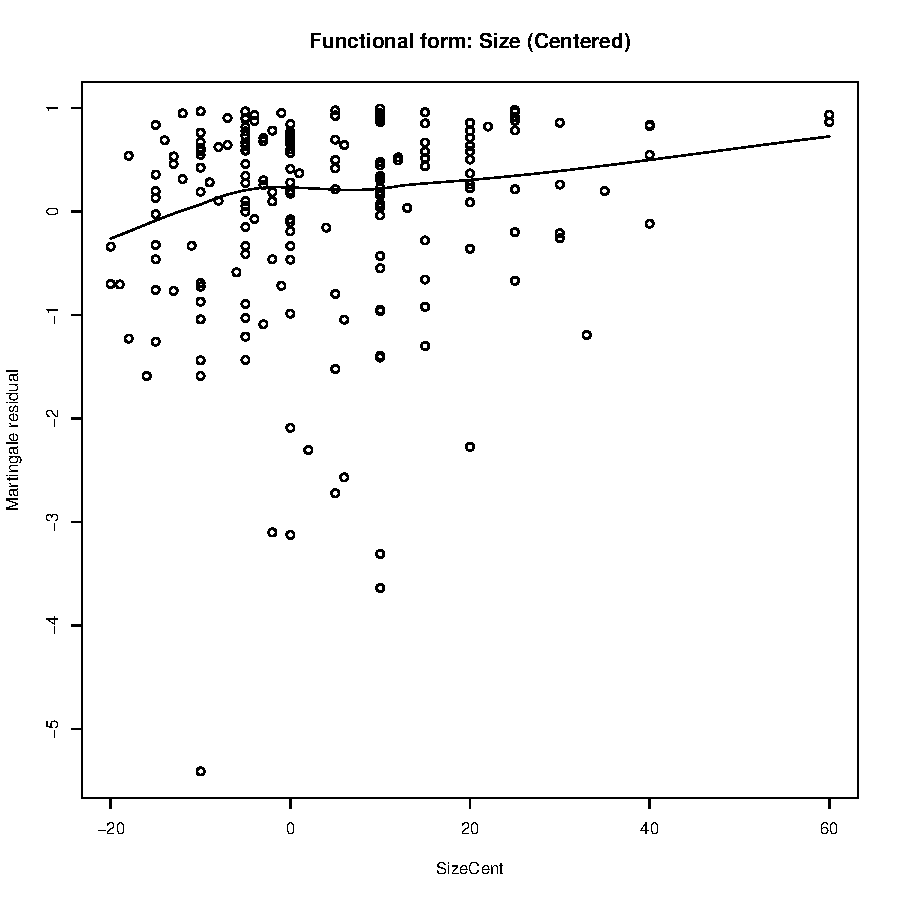
\includegraphics[width=\maxwidth]{figure/eda-func-form-3} 

}


\begin{kframe}\begin{alltt}
\hlkwd{scatter.smooth}\hlstd{(data}\hlopt{$}\hlstd{SizeCent,} \hlkwd{resid}\hlstd{(fit.cph.NoSize,} \hlkwc{type} \hlstd{=} \hlstr{"martingale"}\hlstd{),} \hlkwc{main} \hlstd{=} \hlstr{"Functional form: Size (Centered)"}\hlstd{,}
    \hlkwc{xlab} \hlstd{=} \hlstr{"SizeCent"}\hlstd{,} \hlkwc{ylab} \hlstd{=} \hlstr{"Martingale residual"}\hlstd{,} \hlkwc{ylim} \hlstd{=} \hlkwd{c}\hlstd{(}\hlopt{-}\hlnum{1}\hlstd{,} \hlnum{1}\hlstd{))}
\end{alltt}
\end{kframe}

{\centering 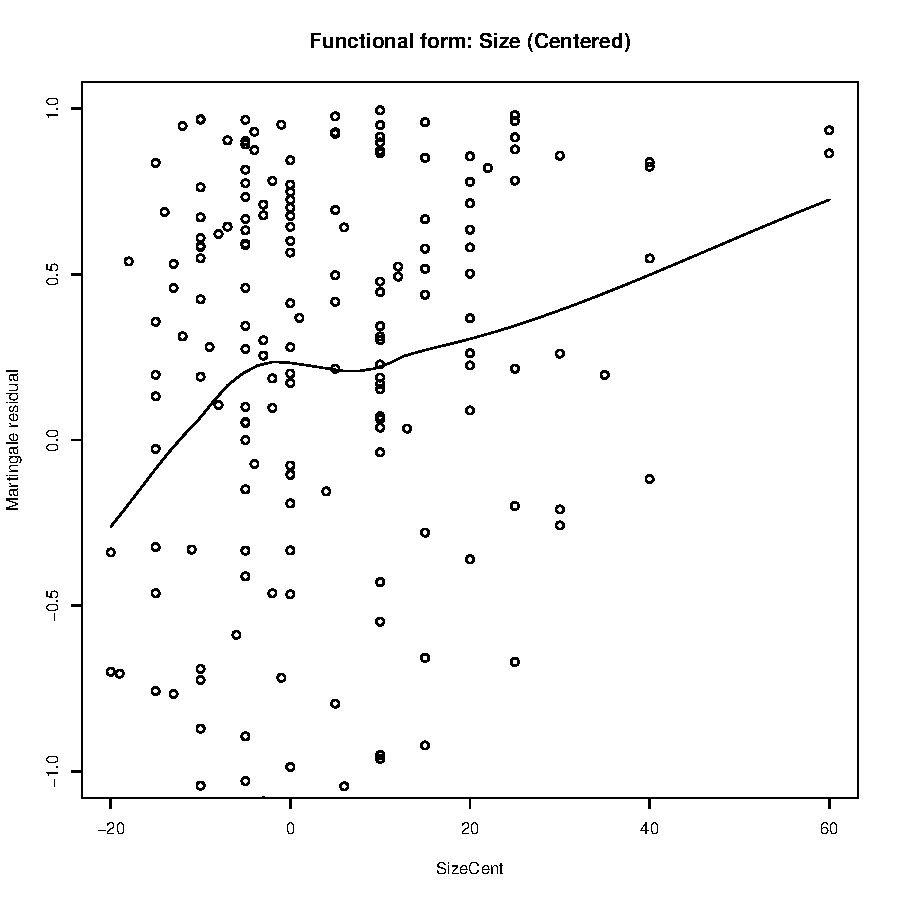
\includegraphics[width=\maxwidth]{figure/eda-func-form-4} 

}



\end{knitrout}
It looks like age has a minor nonlinear component, leading to a quadratic-like U shape.  The size relationship appears to have a knee, close to size == 0, around which the relationship is approximately linear.

Model age as:  $AgeCent + AgeCent^2$
Model size as: $SizeCent + SizeCent I(SizeCent > 0) \equiv SizeCent + SizeCent_+$

\begin{knitrout}
\definecolor{shadecolor}{rgb}{0.969, 0.969, 0.969}\color{fgcolor}\begin{kframe}
\begin{alltt}
\hlstd{data}\hlopt{$}\hlstd{SizeSmall} \hlkwb{=} \hlstd{data}\hlopt{$}\hlstd{SizeCent} \hlopt{*} \hlstd{(data}\hlopt{$}\hlstd{SizeCent} \hlopt{<} \hlnum{0}\hlstd{)}
\end{alltt}
\end{kframe}
\end{knitrout}

\subsection{PH assumption: full model}
\begin{knitrout}
\definecolor{shadecolor}{rgb}{0.969, 0.969, 0.969}\color{fgcolor}\begin{kframe}
\begin{alltt}
\hlstd{fit.cph} \hlkwb{=} \hlkwd{coxph}\hlstd{(}\hlkwd{Surv}\hlstd{(Time, DSD)} \hlopt{~} \hlstd{SexM} \hlopt{+} \hlstd{AgeCent} \hlopt{+} \hlkwd{I}\hlstd{(AgeCent}\hlopt{^}\hlnum{2}\hlstd{)} \hlopt{+} \hlstd{LocBody} \hlopt{+}
    \hlstd{SizeCent} \hlopt{+} \hlstd{SizeSmall} \hlopt{+} \hlstd{A2} \hlopt{+} \hlstd{A4,} \hlkwc{data} \hlstd{= data)}
\hlkwd{cox.zph}\hlstd{(fit.cph)}
\end{alltt}
\begin{verbatim}
##                  rho   chisq      p
## SexMTRUE      0.1520  4.2830 0.0385
## AgeCent      -0.0897  1.5736 0.2097
## I(AgeCent^2)  0.0392  0.2733 0.6012
## LocBodyTRUE  -0.1287  2.7244 0.0988
## SizeCent      0.0088  0.0168 0.8970
## SizeSmall    -0.0592  0.6803 0.4095
## A2TRUE        0.0533  0.5483 0.4590
## A4TRUE       -0.0596  0.6487 0.4206
## GLOBAL            NA 14.0077 0.0816
\end{verbatim}
\begin{alltt}
\hlkwd{plot}\hlstd{(}\hlkwd{cox.zph}\hlstd{(fit.cph))}
\end{alltt}
\end{kframe}

{\centering 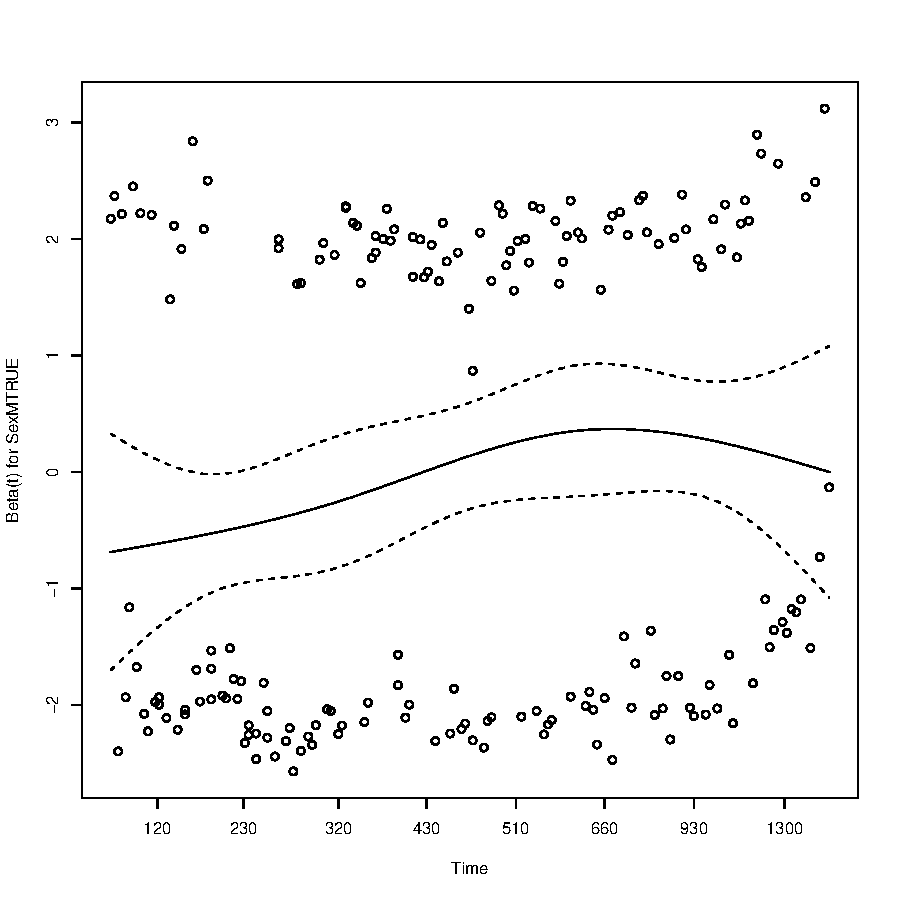
\includegraphics[width=\maxwidth]{figure/eda-ph-check-full-1} 

}




{\centering 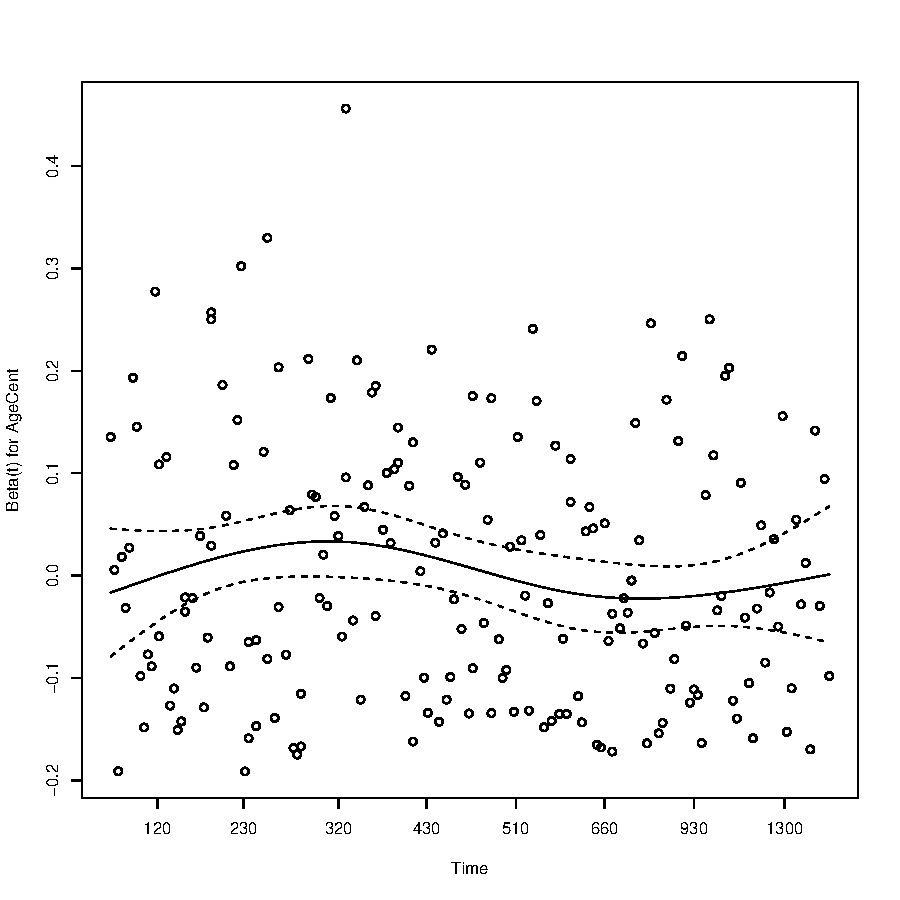
\includegraphics[width=\maxwidth]{figure/eda-ph-check-full-2} 

}




{\centering 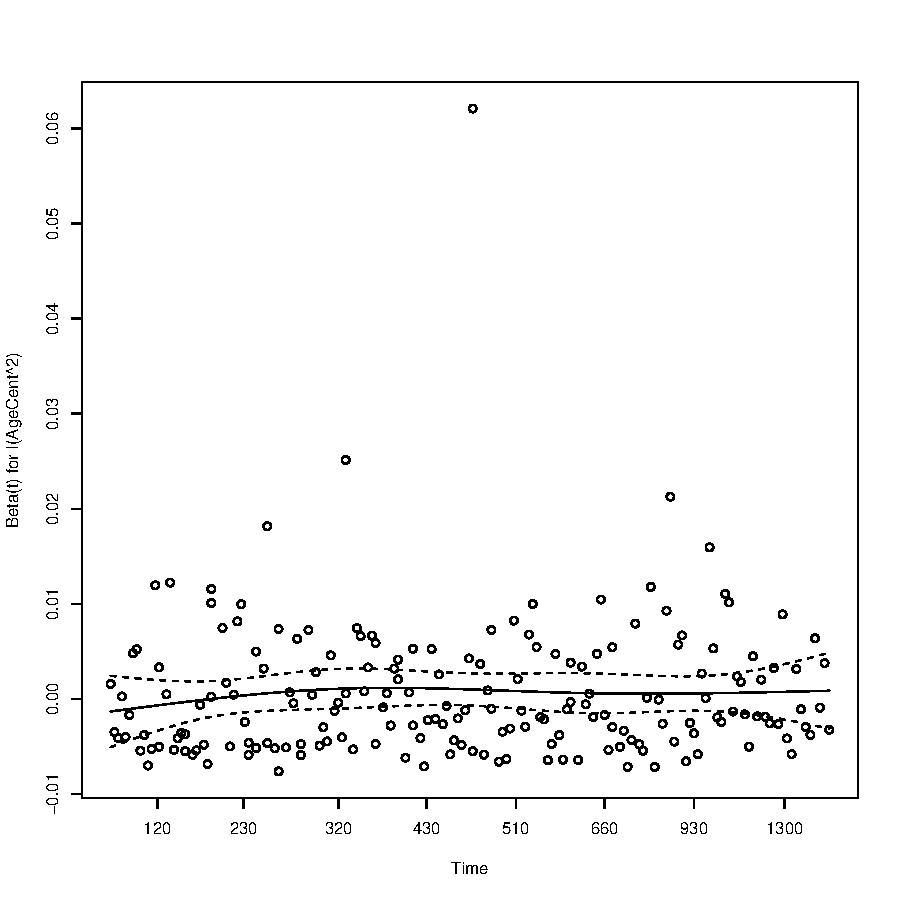
\includegraphics[width=\maxwidth]{figure/eda-ph-check-full-3} 

}




{\centering 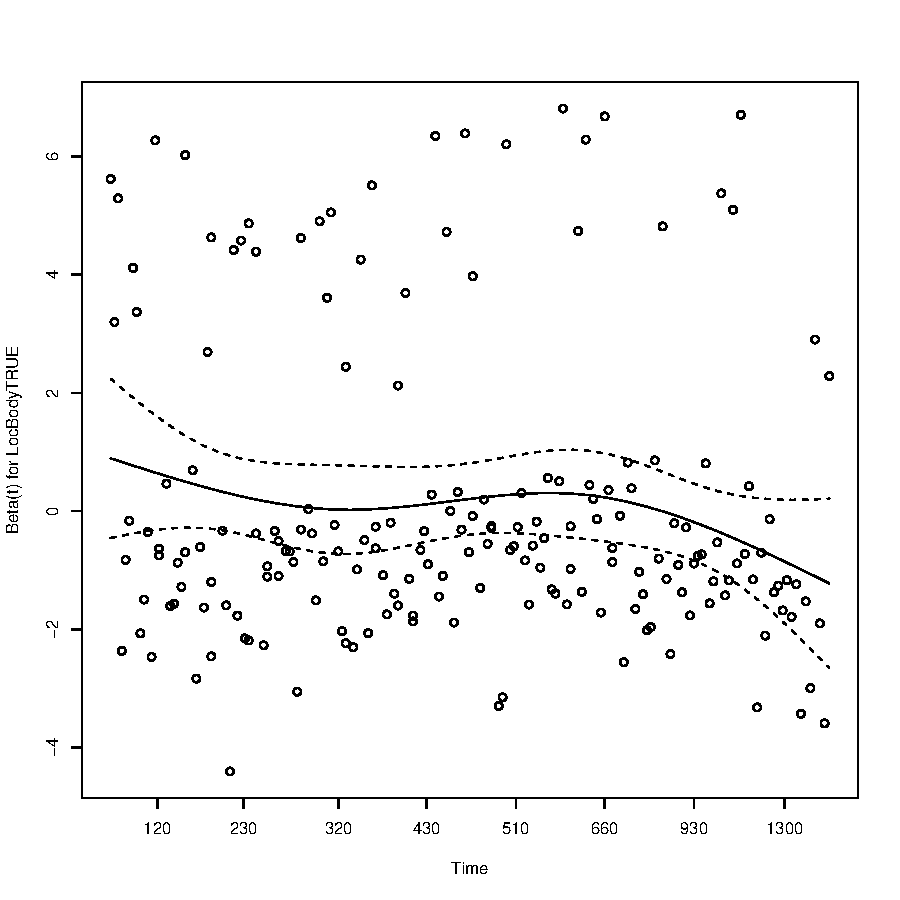
\includegraphics[width=\maxwidth]{figure/eda-ph-check-full-4} 

}




{\centering 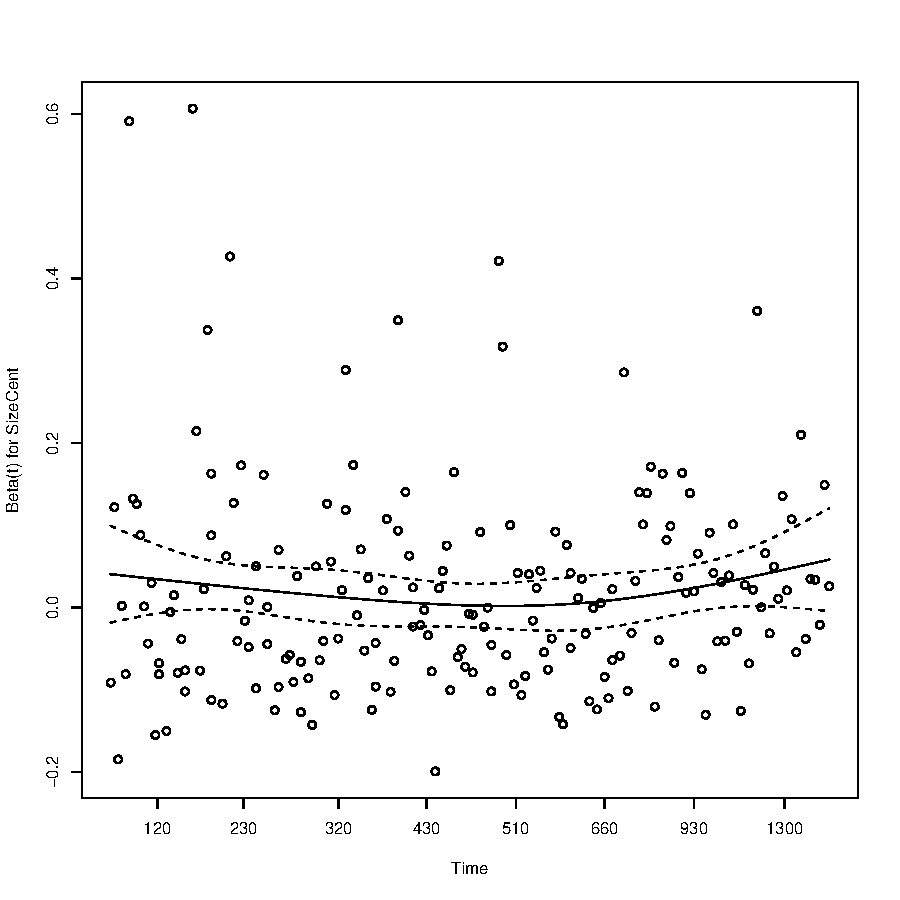
\includegraphics[width=\maxwidth]{figure/eda-ph-check-full-5} 

}




{\centering 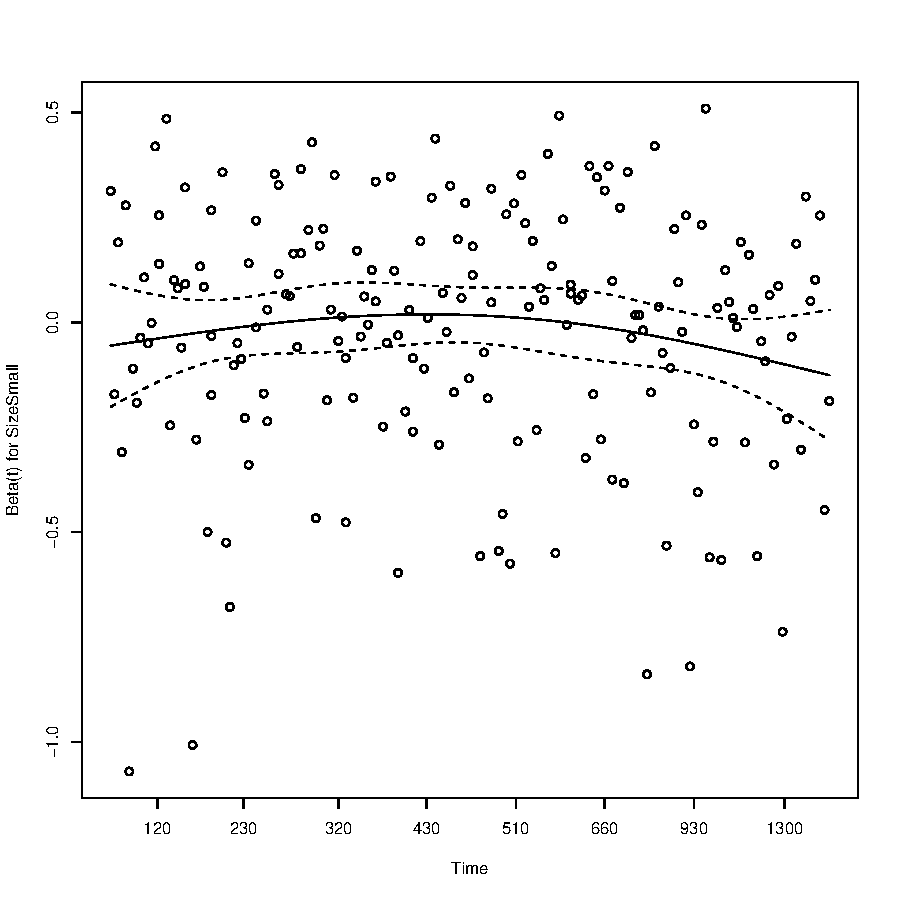
\includegraphics[width=\maxwidth]{figure/eda-ph-check-full-6} 

}




{\centering 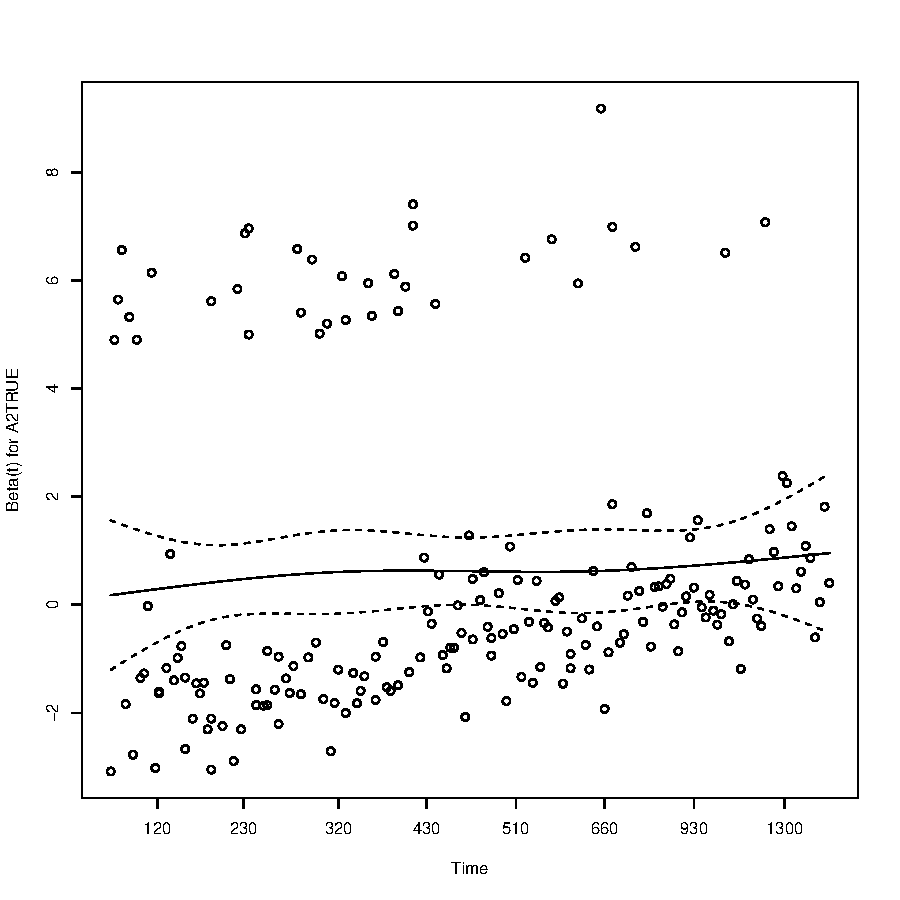
\includegraphics[width=\maxwidth]{figure/eda-ph-check-full-7} 

}




{\centering 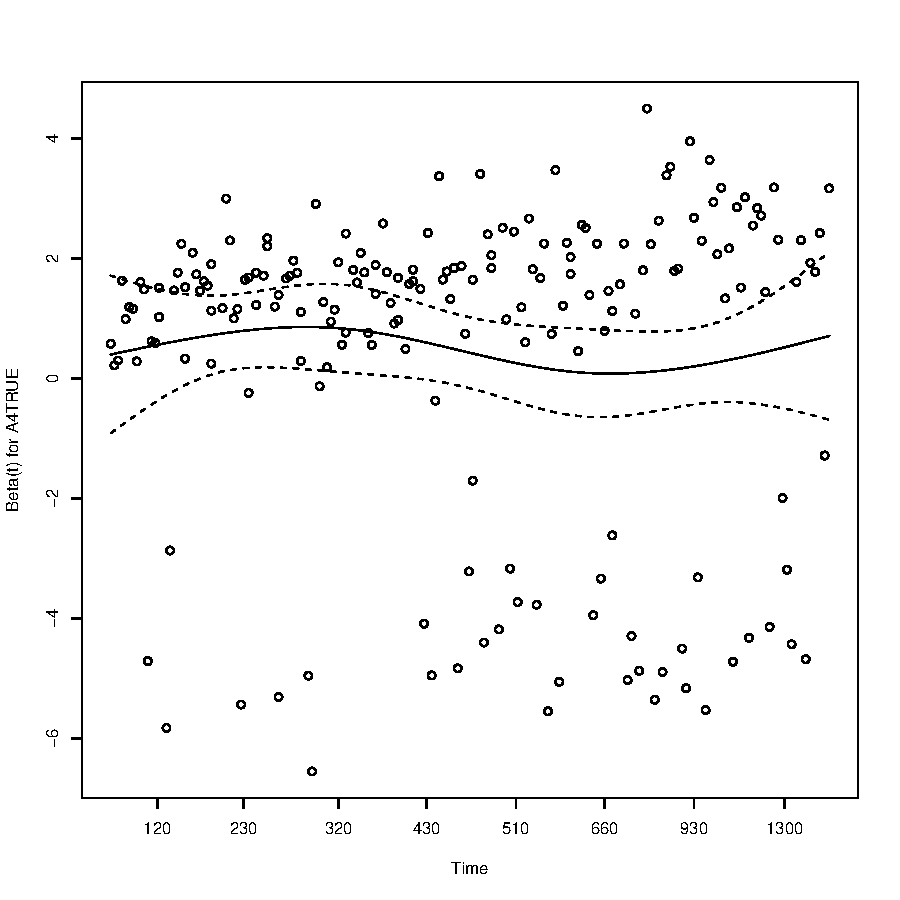
\includegraphics[width=\maxwidth]{figure/eda-ph-check-full-8} 

}



\end{knitrout}

Looks like there's a violation of CPH with gender.  Not unexpected.  First check whether there is any evidence of gender interaction.
\begin{knitrout}
\definecolor{shadecolor}{rgb}{0.969, 0.969, 0.969}\color{fgcolor}\begin{kframe}
\begin{alltt}
\hlkwd{anova}\hlstd{(}\hlkwd{coxph}\hlstd{(}\hlkwd{Surv}\hlstd{(Time, DSD)} \hlopt{~} \hlstd{SexM} \hlopt{*} \hlstd{(AgeCent} \hlopt{+} \hlkwd{I}\hlstd{(AgeCent}\hlopt{^}\hlnum{2}\hlstd{)} \hlopt{+} \hlstd{LocBody} \hlopt{+} \hlstd{SizeCent} \hlopt{+}
    \hlstd{SizeSmall} \hlopt{+} \hlstd{A2} \hlopt{+} \hlstd{A4),} \hlkwc{data} \hlstd{= data))}
\end{alltt}
\begin{verbatim}
## Analysis of Deviance Table
##  Cox model: response is Surv(Time, DSD)
## Terms added sequentially (first to last)
## 
##                   loglik Chisq Df Pr(>|Chi|)
## NULL                -816                    
## SexM                -816  0.31  1     0.5770
## AgeCent             -816  0.00  1     0.9623
## I(AgeCent^2)        -815  0.78  1     0.3773
## LocBody             -813  3.45  1     0.0634
## SizeCent            -809  7.86  1     0.0050
## SizeSmall           -809  0.00  1     0.9983
## A2                  -805  9.64  1     0.0019
## A4                  -801  6.85  1     0.0088
## SexM:AgeCent        -800  1.65  1     0.1993
## SexM:I(AgeCent^2)   -800  0.00  1     0.9808
## SexM:LocBody        -800  0.10  1     0.7568
## SexM:SizeCent       -800  0.65  1     0.4218
## SexM:SizeSmall      -800  0.01  1     0.9108
## SexM:A2             -800  0.00  1     0.9960
## SexM:A4             -800  0.03  1     0.8537
\end{verbatim}
\end{kframe}
\end{knitrout}
Nope, good.  We're not interested in gender effects so just stratify.

\begin{knitrout}
\definecolor{shadecolor}{rgb}{0.969, 0.969, 0.969}\color{fgcolor}\begin{kframe}
\begin{alltt}
\hlstd{fit.cph} \hlkwb{=} \hlkwd{coxph}\hlstd{(}\hlkwd{Surv}\hlstd{(Time, DSD)} \hlopt{~} \hlkwd{strata}\hlstd{(SexM)} \hlopt{+} \hlstd{AgeCent} \hlopt{+} \hlkwd{I}\hlstd{(AgeCent}\hlopt{^}\hlnum{2}\hlstd{)} \hlopt{+} \hlstd{LocBody} \hlopt{+}
    \hlstd{SizeCent} \hlopt{+} \hlstd{SizeSmall} \hlopt{+} \hlstd{A2} \hlopt{+} \hlstd{A4,} \hlkwc{data} \hlstd{= data)}
\hlkwd{cox.zph}\hlstd{(fit.cph)}
\end{alltt}
\begin{verbatim}
##                   rho  chisq     p
## AgeCent      -0.09066 1.6632 0.197
## I(AgeCent^2)  0.03371 0.2006 0.654
## LocBodyTRUE  -0.10840 1.8729 0.171
## SizeCent     -0.00856 0.0157 0.900
## SizeSmall    -0.04531 0.3927 0.531
## A2TRUE        0.05681 0.6145 0.433
## A4TRUE       -0.06539 0.7755 0.379
## GLOBAL             NA 8.3356 0.304
\end{verbatim}
\begin{alltt}
\hlkwd{plot}\hlstd{(}\hlkwd{cox.zph}\hlstd{(fit.cph))}
\end{alltt}
\end{kframe}

{\centering 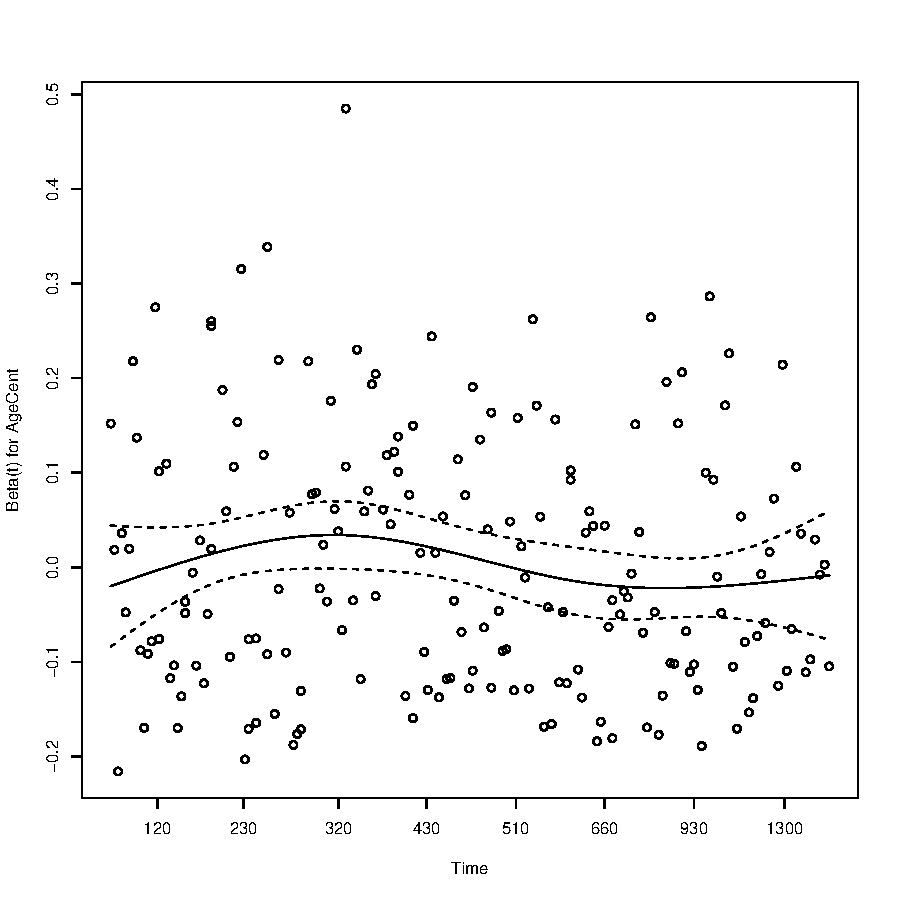
\includegraphics[width=\maxwidth]{figure/eda-ph-check-full-3-1} 

}




{\centering 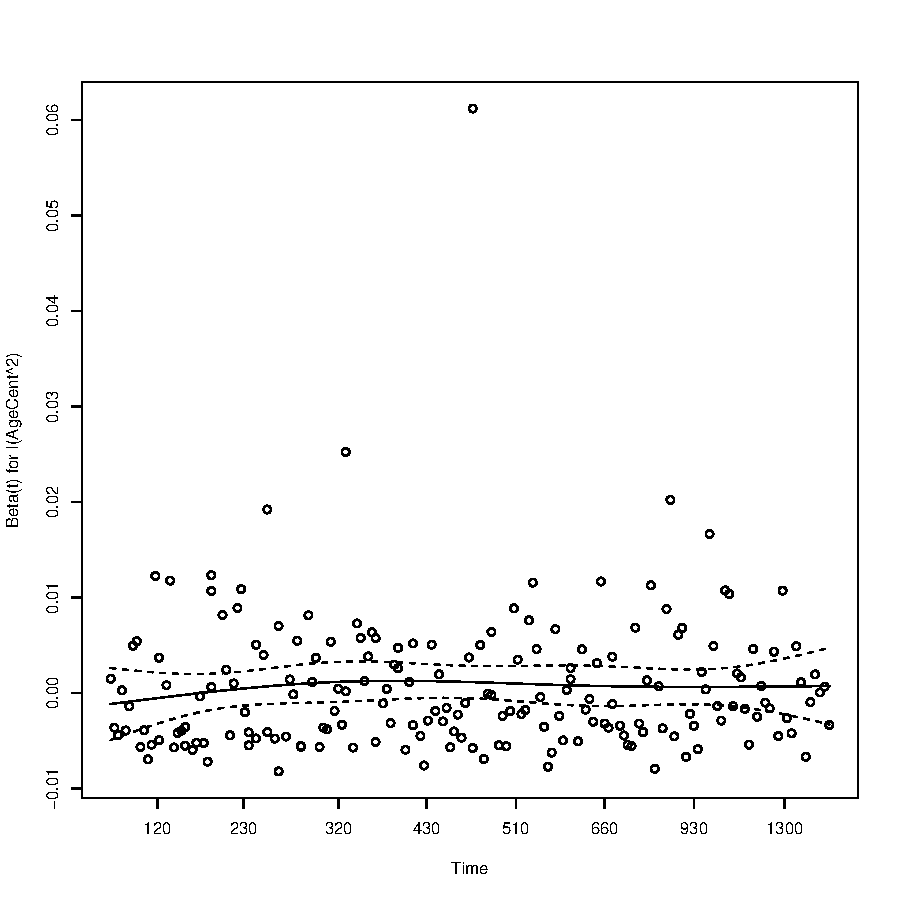
\includegraphics[width=\maxwidth]{figure/eda-ph-check-full-3-2} 

}




{\centering 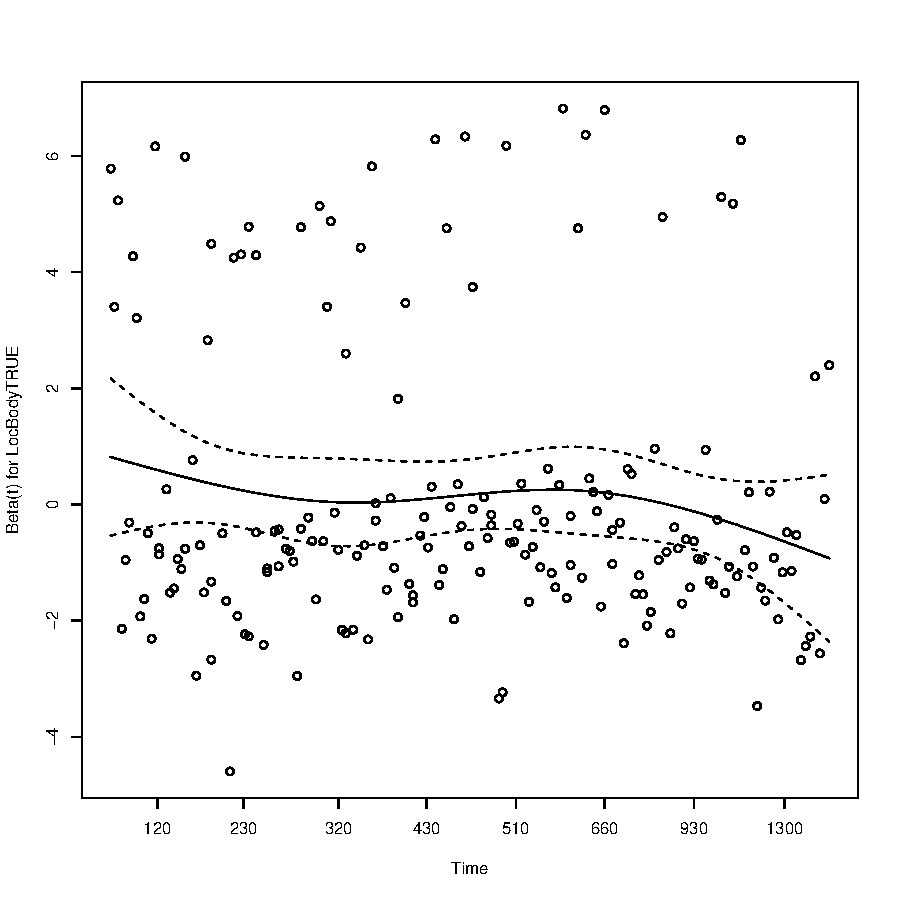
\includegraphics[width=\maxwidth]{figure/eda-ph-check-full-3-3} 

}




{\centering 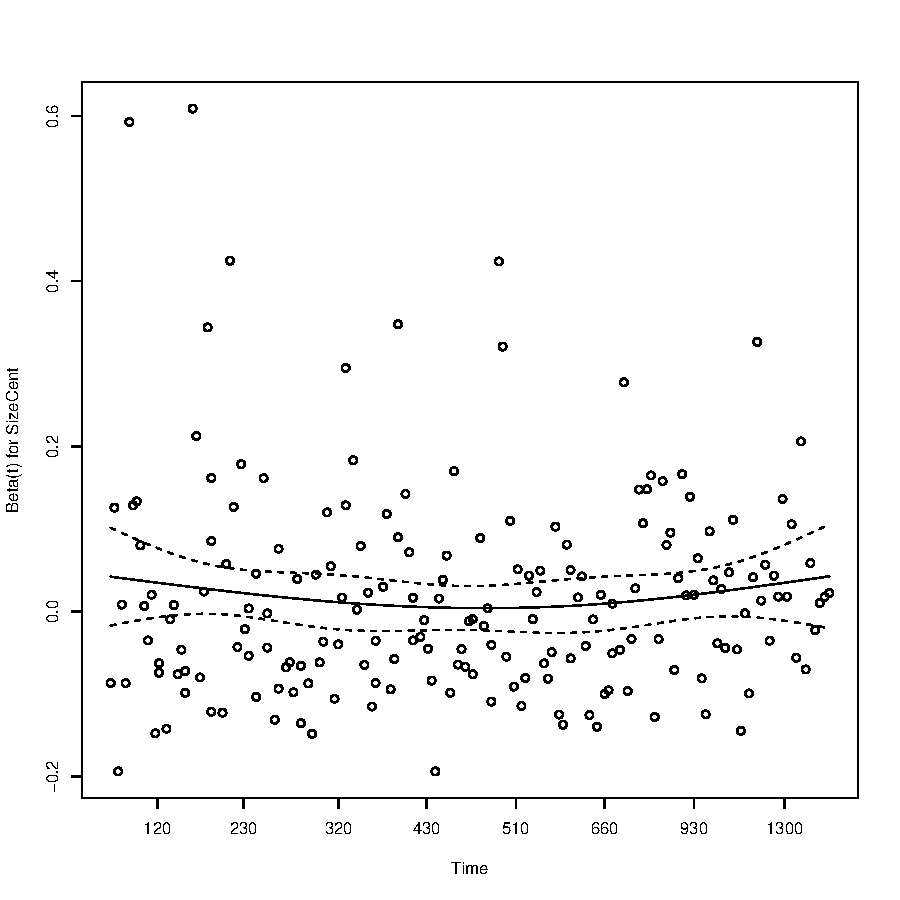
\includegraphics[width=\maxwidth]{figure/eda-ph-check-full-3-4} 

}




{\centering 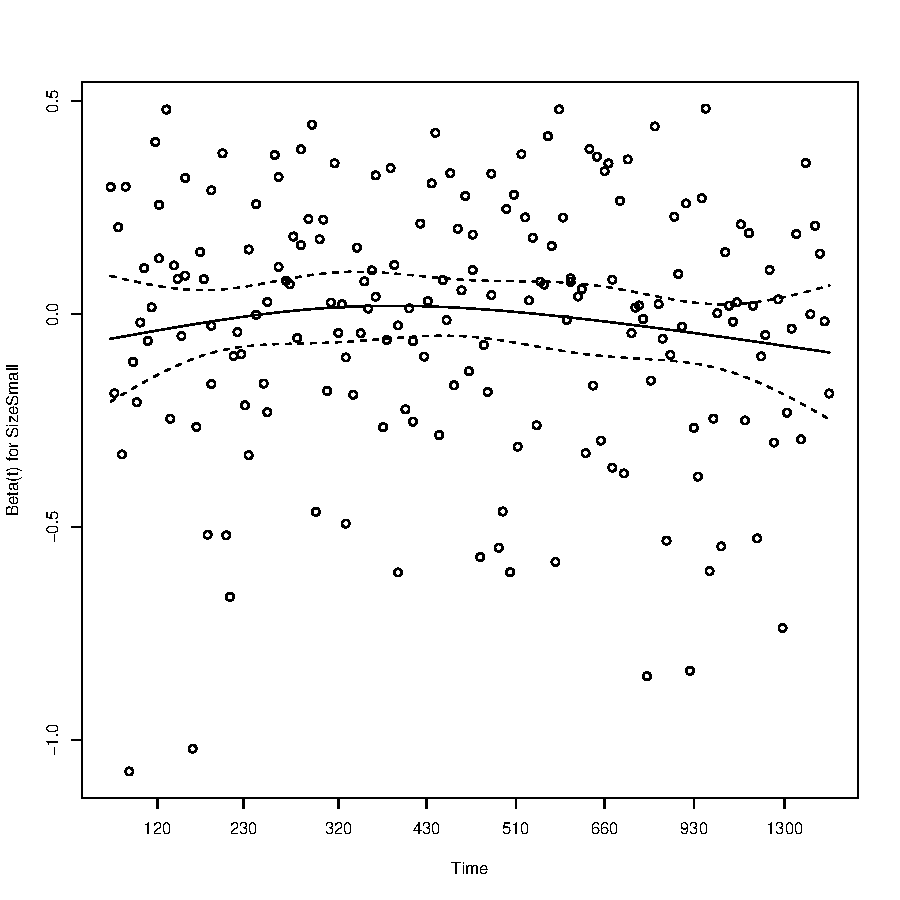
\includegraphics[width=\maxwidth]{figure/eda-ph-check-full-3-5} 

}




{\centering 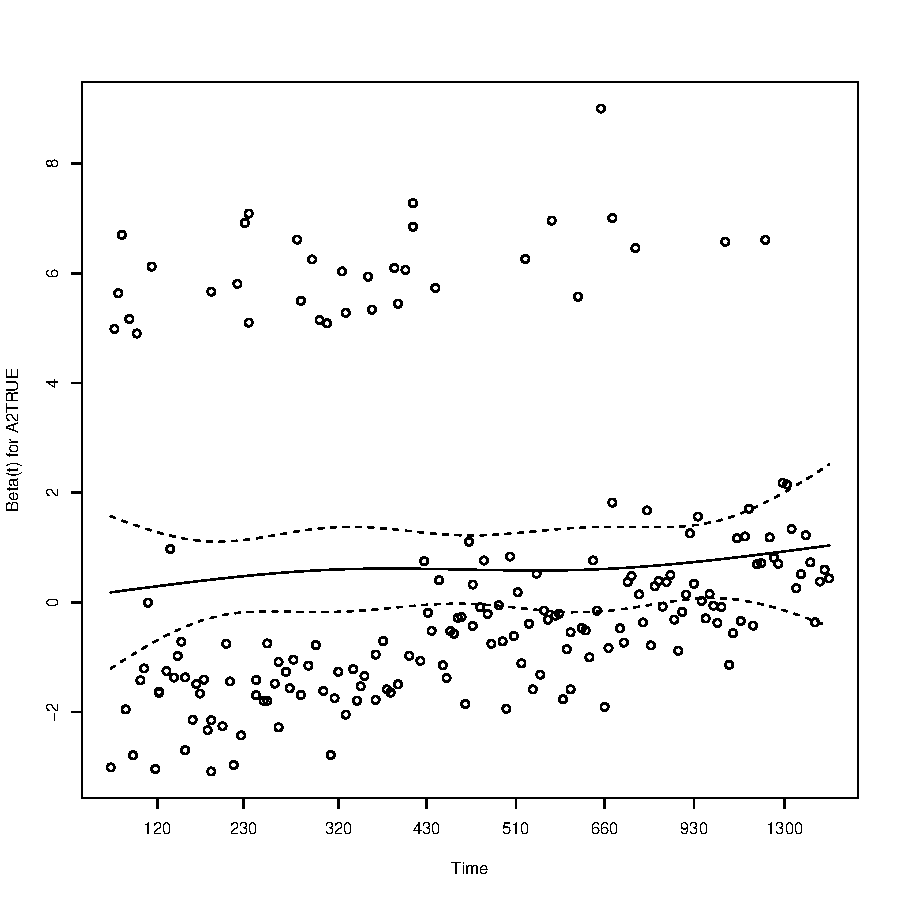
\includegraphics[width=\maxwidth]{figure/eda-ph-check-full-3-6} 

}




{\centering 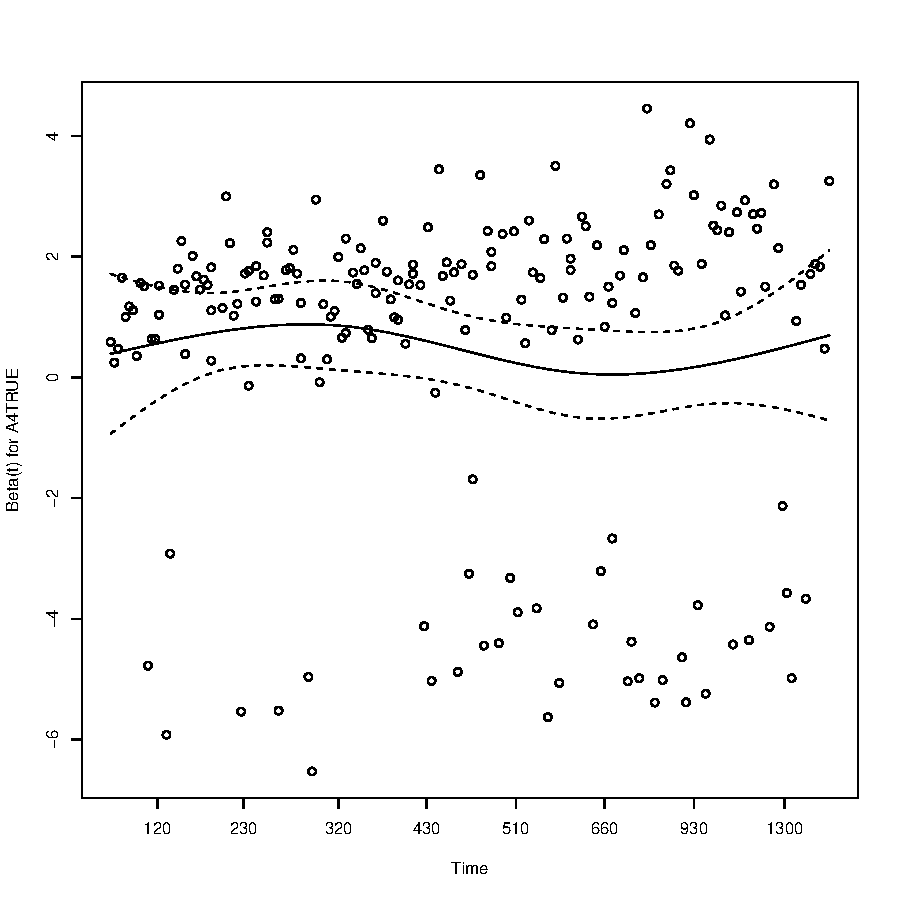
\includegraphics[width=\maxwidth]{figure/eda-ph-check-full-3-7} 

}



\end{knitrout}

Looks good.  Slight snifter with age but I'm not particularly concerned.
Split into age groups and do KM plots to verify.
\begin{knitrout}
\definecolor{shadecolor}{rgb}{0.969, 0.969, 0.969}\color{fgcolor}\begin{kframe}
\begin{alltt}
\hlstd{temp.age} \hlkwb{=} \hlkwd{cut}\hlstd{(data}\hlopt{$}\hlstd{AgeCent,} \hlnum{4}\hlstd{)}
\hlstd{temp} \hlkwb{=} \hlkwd{survfit}\hlstd{(}\hlkwd{Surv}\hlstd{(Time, DSD)} \hlopt{~} \hlstd{temp.age, data)}
\hlkwd{ggplot}\hlstd{(}\hlkwd{data.frame}\hlstd{(}\hlkwc{surv} \hlstd{= temp}\hlopt{$}\hlstd{surv,} \hlkwc{time} \hlstd{= temp}\hlopt{$}\hlstd{time,} \hlkwc{age} \hlstd{=} \hlkwd{rep}\hlstd{(}\hlkwd{names}\hlstd{(temp}\hlopt{$}\hlstd{strata),}
    \hlstd{temp}\hlopt{$}\hlstd{strata)),} \hlkwd{aes}\hlstd{(}\hlkwc{y} \hlstd{=} \hlkwd{log}\hlstd{(}\hlopt{-}\hlkwd{log}\hlstd{(surv)),} \hlkwc{x} \hlstd{=} \hlkwd{log}\hlstd{(time),} \hlkwc{col} \hlstd{= age))} \hlopt{+} \hlkwd{geom_line}\hlstd{()}
\end{alltt}
\end{kframe}

{\centering 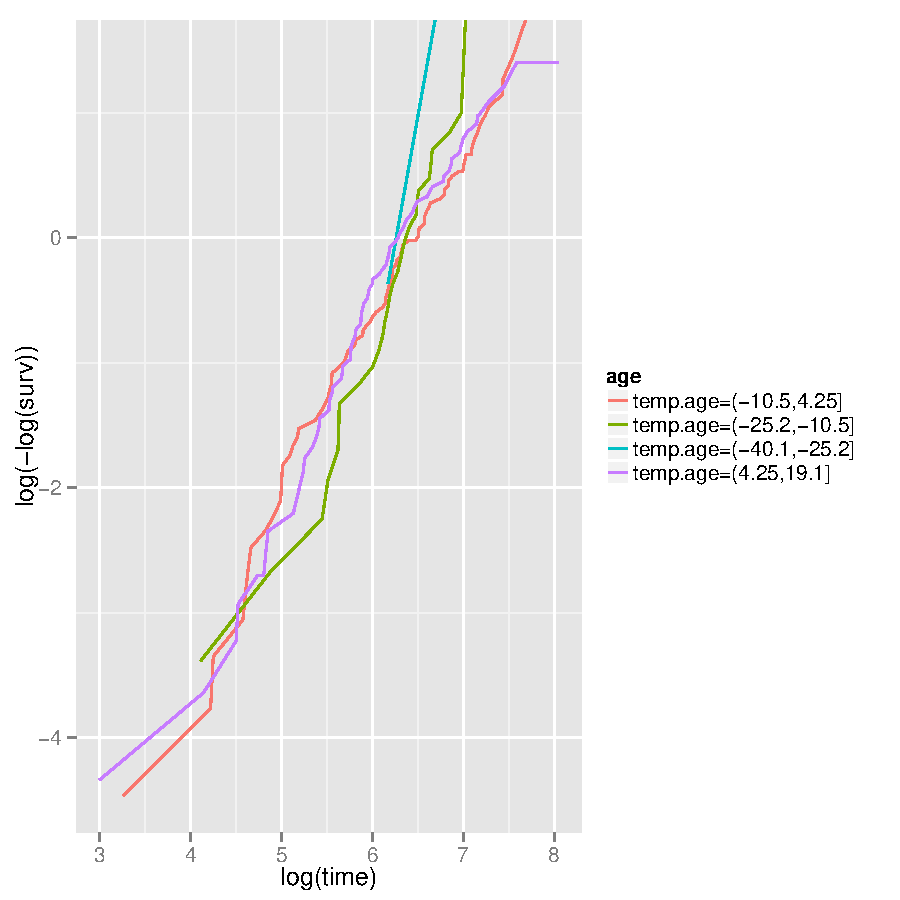
\includegraphics[width=\maxwidth]{figure/eda-ph-check-full-age-1} 

}



\end{knitrout}
Not perfect but it'll do.


\subsection{Outliers: full model}
Look at deviance residuals, both marginally and stratified by major subgroups.
\begin{knitrout}
\definecolor{shadecolor}{rgb}{0.969, 0.969, 0.969}\color{fgcolor}\begin{kframe}
\begin{alltt}
\hlkwd{plot}\hlstd{(}\hlkwd{resid}\hlstd{(fit.cph,} \hlkwc{type} \hlstd{=} \hlstr{"deviance"}\hlstd{))}
\hlkwd{abline}\hlstd{(}\hlkwc{h} \hlstd{=} \hlkwd{c}\hlstd{(}\hlopt{-}\hlnum{2.5}\hlstd{,} \hlnum{2.5}\hlstd{))}
\end{alltt}
\end{kframe}

{\centering 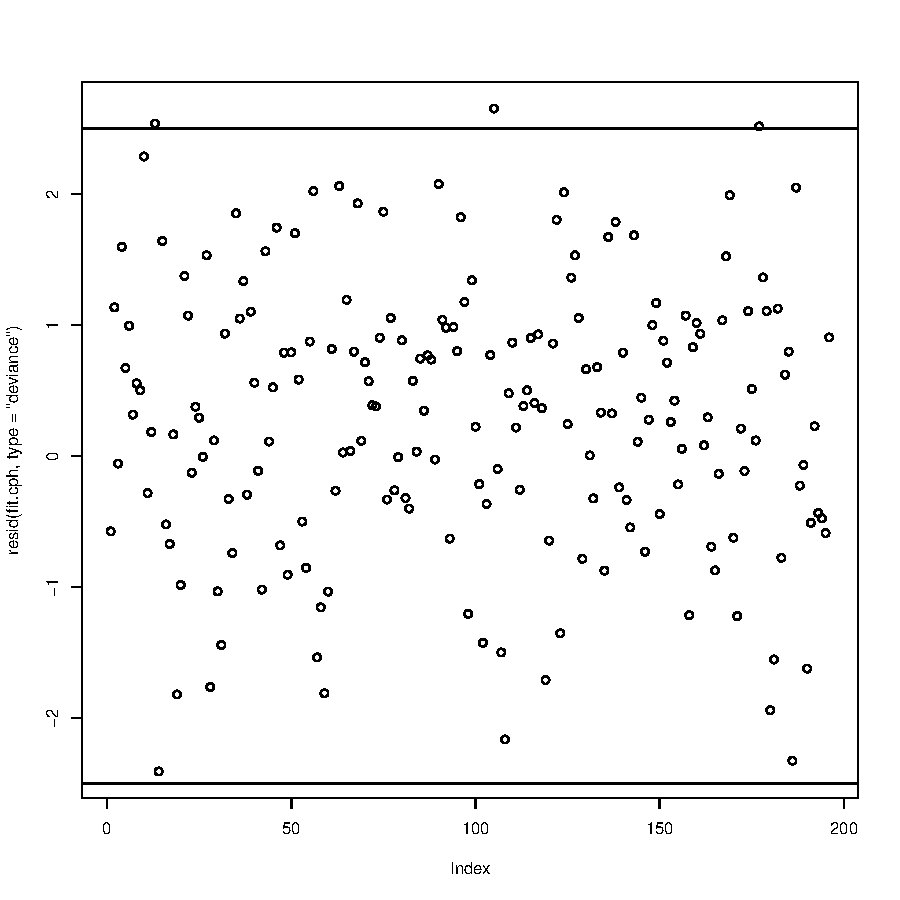
\includegraphics[width=\maxwidth]{figure/eda-outliers-full-1} 

}


\begin{kframe}\begin{alltt}
\hlkwd{plot}\hlstd{(}\hlkwd{resid}\hlstd{(fit.cph,} \hlkwc{type} \hlstd{=} \hlstr{"deviance"}\hlstd{)[}\hlkwd{order}\hlstd{(data}\hlopt{$}\hlstd{SexM, data}\hlopt{$}\hlstd{A2, data}\hlopt{$}\hlstd{A4)],}
    \hlkwc{col} \hlstd{= (}\hlnum{4} \hlopt{*} \hlstd{data}\hlopt{$}\hlstd{SexM} \hlopt{+} \hlnum{2} \hlopt{*} \hlstd{data}\hlopt{$}\hlstd{A2} \hlopt{+} \hlstd{data}\hlopt{$}\hlstd{A4} \hlopt{+} \hlnum{1}\hlstd{)[}\hlkwd{order}\hlstd{(data}\hlopt{$}\hlstd{SexM, data}\hlopt{$}\hlstd{A2,}
        \hlstd{data}\hlopt{$}\hlstd{A4)],} \hlkwc{pch} \hlstd{=} \hlnum{16}\hlstd{)}
\hlkwd{abline}\hlstd{(}\hlkwc{h} \hlstd{=} \hlkwd{c}\hlstd{(}\hlopt{-}\hlnum{2.5}\hlstd{,} \hlnum{2.5}\hlstd{))}
\end{alltt}
\end{kframe}

{\centering 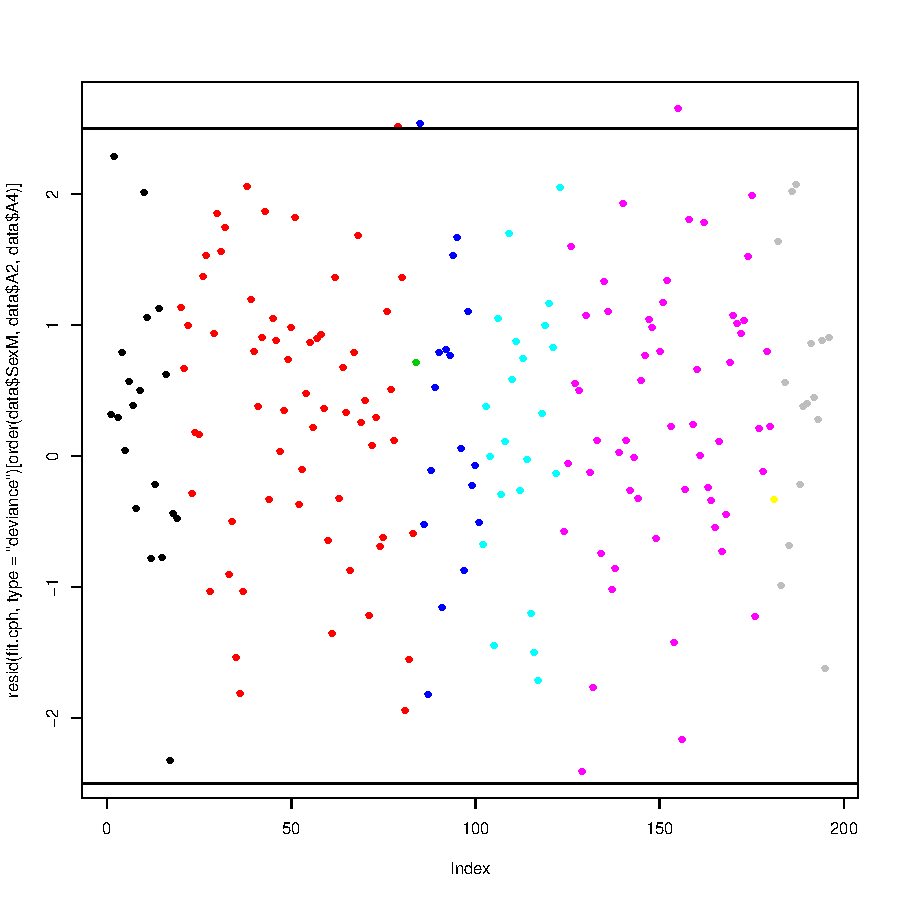
\includegraphics[width=\maxwidth]{figure/eda-outliers-full-2} 

}


\begin{kframe}\begin{alltt}
\hlkwd{boxplot}\hlstd{(}\hlkwd{resid}\hlstd{(fit.cph,} \hlkwc{type} \hlstd{=} \hlstr{"deviance"}\hlstd{)} \hlopt{~} \hlstd{data}\hlopt{$}\hlstd{SexM} \hlopt{+} \hlstd{data}\hlopt{$}\hlstd{A2} \hlopt{+} \hlstd{data}\hlopt{$}\hlstd{A4,} \hlkwc{varwidth} \hlstd{=} \hlnum{TRUE}\hlstd{)}
\hlkwd{abline}\hlstd{(}\hlkwc{h} \hlstd{=} \hlnum{0}\hlstd{)}
\end{alltt}
\end{kframe}

{\centering 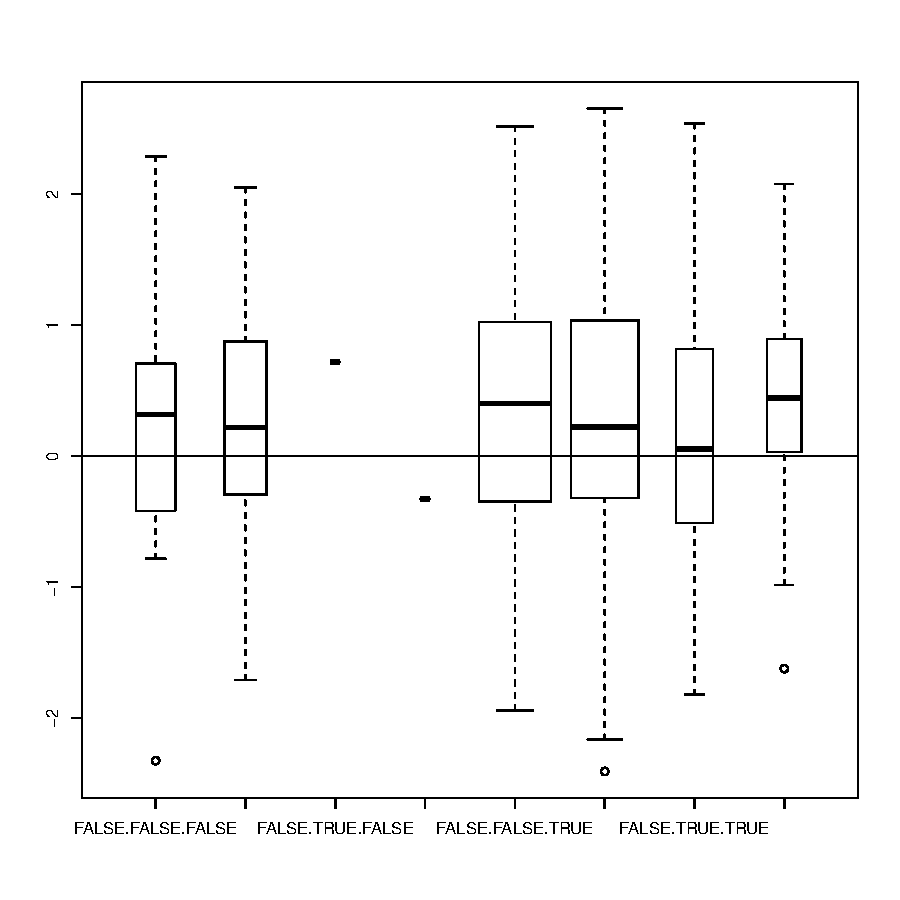
\includegraphics[width=\maxwidth]{figure/eda-outliers-full-3} 

}


\begin{kframe}\begin{alltt}
\hlkwd{boxplot}\hlstd{(}\hlkwd{resid}\hlstd{(fit.cph,} \hlkwc{type} \hlstd{=} \hlstr{"martingale"}\hlstd{)} \hlopt{~} \hlstd{data}\hlopt{$}\hlstd{SexM} \hlopt{+} \hlstd{data}\hlopt{$}\hlstd{A2} \hlopt{+} \hlstd{data}\hlopt{$}\hlstd{A4,}
    \hlkwc{varwidth} \hlstd{=} \hlnum{TRUE}\hlstd{)}
\hlkwd{abline}\hlstd{(}\hlkwc{h} \hlstd{=} \hlnum{0}\hlstd{)}
\end{alltt}
\end{kframe}

{\centering 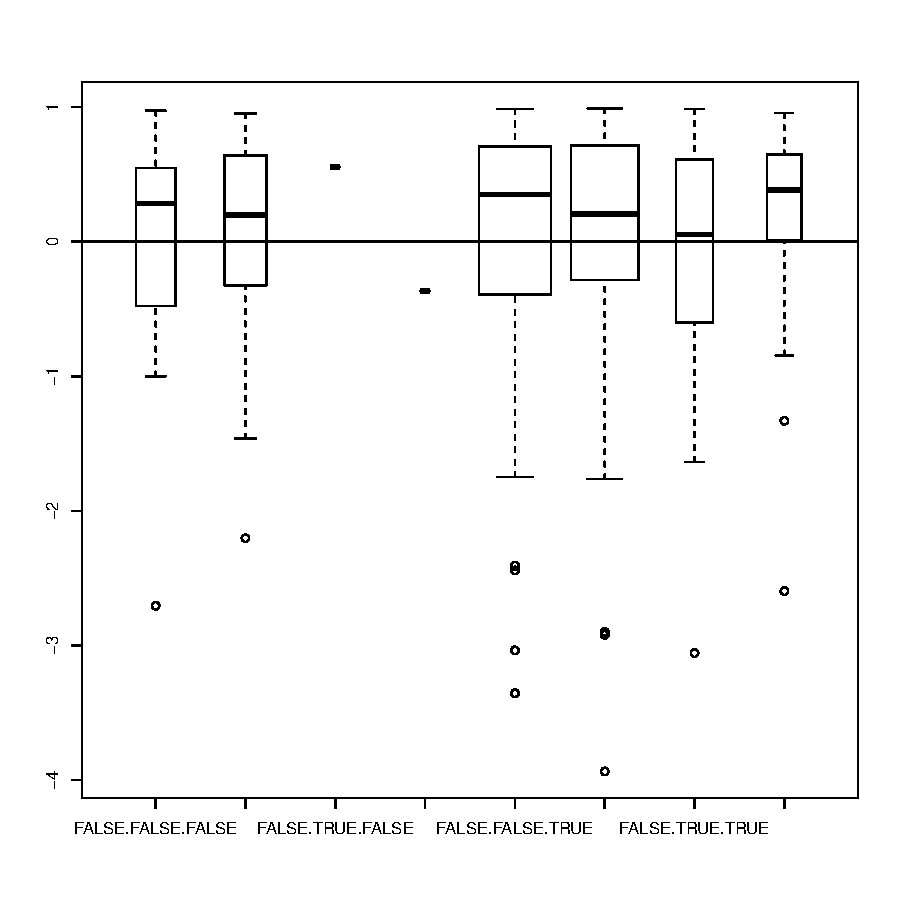
\includegraphics[width=\maxwidth]{figure/eda-outliers-full-4} 

}



\end{knitrout}

Use DFBETAS to examine influence.
\begin{knitrout}
\definecolor{shadecolor}{rgb}{0.969, 0.969, 0.969}\color{fgcolor}\begin{kframe}
\begin{alltt}
\hlstd{temp} \hlkwb{=} \hlkwd{resid}\hlstd{(fit.cph,} \hlkwc{type} \hlstd{=} \hlstr{"dfbetas"}\hlstd{)}
\hlkwd{colnames}\hlstd{(temp)} \hlkwb{=} \hlkwd{names}\hlstd{(fit.cph}\hlopt{$}\hlstd{coefficients)}
\hlstd{temp} \hlkwb{=} \hlkwd{melt}\hlstd{(temp)}
\hlkwd{colnames}\hlstd{(temp)} \hlkwb{=} \hlkwd{c}\hlstd{(}\hlstr{"Patient"}\hlstd{,} \hlstr{"Coefficient"}\hlstd{,} \hlstr{"dfbetas"}\hlstd{)}
\hlkwd{ggplot}\hlstd{(temp,} \hlkwd{aes}\hlstd{(}\hlkwc{y} \hlstd{= dfbetas,} \hlkwc{x} \hlstd{= Patient,} \hlkwc{col} \hlstd{= Coefficient))} \hlopt{+} \hlkwd{geom_point}\hlstd{()}
\end{alltt}
\end{kframe}

{\centering 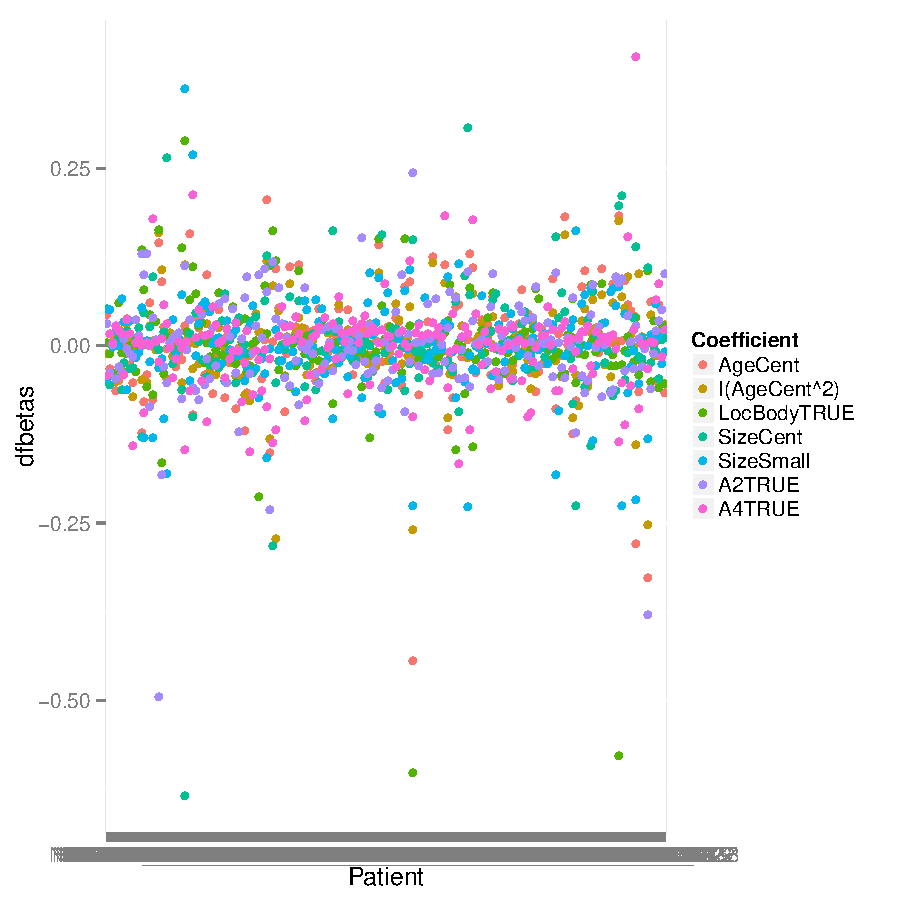
\includegraphics[width=\maxwidth]{figure/eda-dfbetas-full-1} 

}



\end{knitrout}
There is quite a number of rather influential observations.  These could do with some checking, but first collapse down the model -- there's little point doing dfbeta fucking about based on coefficients that will never get fit in the end anyway.


\subsection{EDA: Variable selection}
\begin{knitrout}
\definecolor{shadecolor}{rgb}{0.969, 0.969, 0.969}\color{fgcolor}\begin{kframe}
\begin{alltt}
\hlstd{nobs.coxph} \hlkwb{<<-} \hlkwa{function}\hlstd{(}\hlkwc{obj}\hlstd{,} \hlkwc{...}\hlstd{)} \hlkwd{sum}\hlstd{(obj}\hlopt{$}\hlstd{y[,} \hlnum{2}\hlstd{])}
\hlcom{# Note: Exhaustive search at level 2 is only feasible for at most 5}
\hlcom{# variables fit.cph.as = glmulti(Surv(Time, DSD) ~ strata(SexM) + AgeCent +}
\hlcom{# I(AgeCent^2) + LocBody + SizeCent + SizeSmall + A2 + A4, data = data,}
\hlcom{# marginality = TRUE, method = 'h', fitfunction = 'coxph', crit = 'bic',}
\hlcom{# level = 2)}
\hlkwd{set.seed}\hlstd{(}\hlnum{20150110}\hlstd{)}
\hlstd{fit.cph.as} \hlkwb{=} \hlkwd{glmulti}\hlstd{(}\hlkwd{Surv}\hlstd{(Time, DSD)} \hlopt{~} \hlkwd{strata}\hlstd{(SexM)} \hlopt{+} \hlstd{AgeCent} \hlopt{+} \hlkwd{I}\hlstd{(AgeCent}\hlopt{^}\hlnum{2}\hlstd{)} \hlopt{+}
    \hlstd{LocBody} \hlopt{+} \hlstd{SizeCent} \hlopt{+} \hlstd{SizeSmall} \hlopt{+} \hlstd{A2} \hlopt{+} \hlstd{A4,} \hlkwc{data} \hlstd{= data,} \hlkwc{marginality} \hlstd{=} \hlnum{TRUE}\hlstd{,}
    \hlkwc{method} \hlstd{=} \hlstr{"g"}\hlstd{,} \hlkwc{fitfunction} \hlstd{=} \hlstr{"coxph"}\hlstd{,} \hlkwc{crit} \hlstd{=} \hlstr{"bic"}\hlstd{,} \hlkwc{level} \hlstd{=} \hlnum{2}\hlstd{,} \hlkwc{plotty} \hlstd{=} \hlnum{FALSE}\hlstd{,}
    \hlkwc{report} \hlstd{=} \hlnum{FALSE}\hlstd{)}
\end{alltt}
\begin{verbatim}
## TASK: Genetic algorithm in the candidate set.
## Initialization...
## Algorithm started...
\end{verbatim}


{\ttfamily\noindent\color{warningcolor}{\#\# Warning in fitter(X, Y, strats, offset, init, control, weights = weights, : Loglik converged before variable\ \ 17 ; beta may be infinite.}}

{\ttfamily\noindent\color{warningcolor}{\#\# Warning in fitter(X, Y, strats, offset, init, control, weights = weights, : Loglik converged before variable\ \ 12 ; beta may be infinite.}}

{\ttfamily\noindent\color{warningcolor}{\#\# Warning in fitter(X, Y, strats, offset, init, control, weights = weights, : Loglik converged before variable\ \ 22 ; beta may be infinite.}}

{\ttfamily\noindent\color{warningcolor}{\#\# Warning in fitter(X, Y, strats, offset, init, control, weights = weights, : Loglik converged before variable\ \ 11 ; beta may be infinite.}}

{\ttfamily\noindent\color{warningcolor}{\#\# Warning in fitter(X, Y, strats, offset, init, control, weights = weights, : Loglik converged before variable\ \ 18 ; beta may be infinite.}}

{\ttfamily\noindent\color{warningcolor}{\#\# Warning in fitter(X, Y, strats, offset, init, control, weights = weights, : Loglik converged before variable\ \ 18 ; beta may be infinite.}}

{\ttfamily\noindent\color{warningcolor}{\#\# Warning in fitter(X, Y, strats, offset, init, control, weights = weights, : Loglik converged before variable\ \ 22 ; beta may be infinite.}}

{\ttfamily\noindent\color{warningcolor}{\#\# Warning in fitter(X, Y, strats, offset, init, control, weights = weights, : Loglik converged before variable\ \ 18 ; beta may be infinite.}}

{\ttfamily\noindent\color{warningcolor}{\#\# Warning in fitter(X, Y, strats, offset, init, control, weights = weights, : Loglik converged before variable\ \ 19 ; beta may be infinite.}}

{\ttfamily\noindent\color{warningcolor}{\#\# Warning in fitter(X, Y, strats, offset, init, control, weights = weights, : Loglik converged before variable\ \ 11 ; beta may be infinite.}}

{\ttfamily\noindent\color{warningcolor}{\#\# Warning in fitter(X, Y, strats, offset, init, control, weights = weights, : Loglik converged before variable\ \ 18 ; beta may be infinite.}}\begin{verbatim}
## Improvements in best and average IC have bebingo en below the specified goals.
## Algorithm is declared to have converged.
## Completed.
\end{verbatim}
\begin{alltt}
\hlcom{# fit.cph.as After 830 generations: Best model:}
\hlcom{# Surv(Time,DSD)~1+strata(SexM)+SizeCent+A2+A4 Crit= 1367.16344569113 Mean}
\hlcom{# crit= 1401.37248769175 Improvements in best and average IC have bebingo en}
\hlcom{# below the specified goals.  Algorithm is declared to have converged.}
\hlcom{# Completed.}
\hlkwd{rm}\hlstd{(nobs.coxph)}
\end{alltt}
\end{kframe}
\end{knitrout}

Also run BIC stepwise, because we can.
\begin{knitrout}
\definecolor{shadecolor}{rgb}{0.969, 0.969, 0.969}\color{fgcolor}\begin{kframe}
\begin{alltt}
\hlkwd{stepAIC}\hlstd{(fit.cph,} \hlkwc{k} \hlstd{=} \hlkwd{log}\hlstd{(}\hlkwd{nrow}\hlstd{(data)))}
\end{alltt}
\begin{verbatim}
## Start:  AIC=1386
## Surv(Time, DSD) ~ strata(SexM) + AgeCent + I(AgeCent^2) + LocBody + 
##     SizeCent + SizeSmall + A2 + A4
## 
##                Df  AIC
## - AgeCent       1 1381
## - LocBody       1 1381
## - SizeSmall     1 1381
## - I(AgeCent^2)  1 1382
## - SizeCent      1 1385
## <none>            1386
## - A4            1 1387
## - A2            1 1388
## 
## Step:  AIC=1381
## Surv(Time, DSD) ~ strata(SexM) + I(AgeCent^2) + LocBody + SizeCent + 
##     SizeSmall + A2 + A4
## 
##                Df  AIC
## - LocBody       1 1376
## - SizeSmall     1 1376
## - I(AgeCent^2)  1 1377
## - SizeCent      1 1379
## <none>            1381
## - A4            1 1382
## - A2            1 1383
## 
## Step:  AIC=1376
## Surv(Time, DSD) ~ strata(SexM) + I(AgeCent^2) + SizeCent + SizeSmall + 
##     A2 + A4
## 
##                Df  AIC
## - SizeSmall     1 1371
## - I(AgeCent^2)  1 1372
## - SizeCent      1 1375
## <none>            1376
## - A4            1 1377
## - A2            1 1379
## 
## Step:  AIC=1371
## Surv(Time, DSD) ~ strata(SexM) + I(AgeCent^2) + SizeCent + A2 + 
##     A4
## 
##                Df  AIC
## - I(AgeCent^2)  1 1367
## <none>            1371
## - SizeCent      1 1371
## - A4            1 1372
## - A2            1 1374
## 
## Step:  AIC=1367
## Surv(Time, DSD) ~ strata(SexM) + SizeCent + A2 + A4
## 
##            Df  AIC
## <none>        1367
## - A4        1 1368
## - SizeCent  1 1368
## - A2        1 1370
## Call:
## coxph(formula = Surv(Time, DSD) ~ strata(SexM) + SizeCent + A2 + 
##     A4, data = data)
## 
## 
##            coef exp(coef) se(coef)    z      p
## SizeCent 0.0139      1.01  0.00563 2.47 0.0140
## A2TRUE   0.5845      1.79  0.19894 2.94 0.0033
## A4TRUE   0.4311      1.54  0.18733 2.30 0.0210
## 
## Likelihood ratio test=25.7  on 3 df, p=1.08e-05  n= 196, number of events= 188
\end{verbatim}
\end{kframe}
\end{knitrout}
Consensus, excellent.


\subsection{PH assumption: reduced model}
\begin{knitrout}
\definecolor{shadecolor}{rgb}{0.969, 0.969, 0.969}\color{fgcolor}\begin{kframe}
\begin{alltt}
\hlstd{fit.cph} \hlkwb{=} \hlkwd{coxph}\hlstd{(}\hlkwd{Surv}\hlstd{(Time, DSD)} \hlopt{~} \hlkwd{strata}\hlstd{(SexM)} \hlopt{+} \hlstd{SizeCent} \hlopt{+} \hlstd{A2} \hlopt{+} \hlstd{A4,} \hlkwc{data} \hlstd{= data)}
\hlkwd{cox.zph}\hlstd{(fit.cph)}
\end{alltt}
\begin{verbatim}
##              rho chisq     p
## SizeCent -0.0937 1.894 0.169
## A2TRUE    0.0248 0.115 0.734
## A4TRUE   -0.0890 1.430 0.232
## GLOBAL        NA 3.747 0.290
\end{verbatim}
\begin{alltt}
\hlkwd{plot}\hlstd{(}\hlkwd{cox.zph}\hlstd{(fit.cph))}
\end{alltt}
\end{kframe}

{\centering 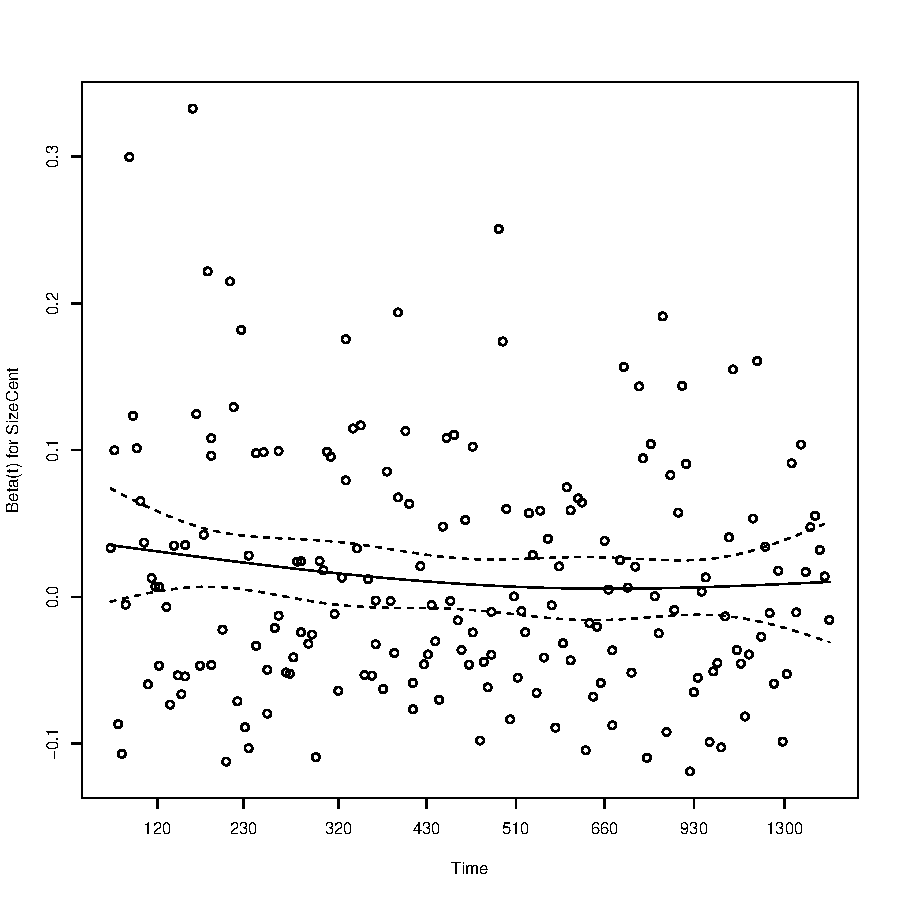
\includegraphics[width=\maxwidth]{figure/eda-ph-check-reduced-1} 

}




{\centering 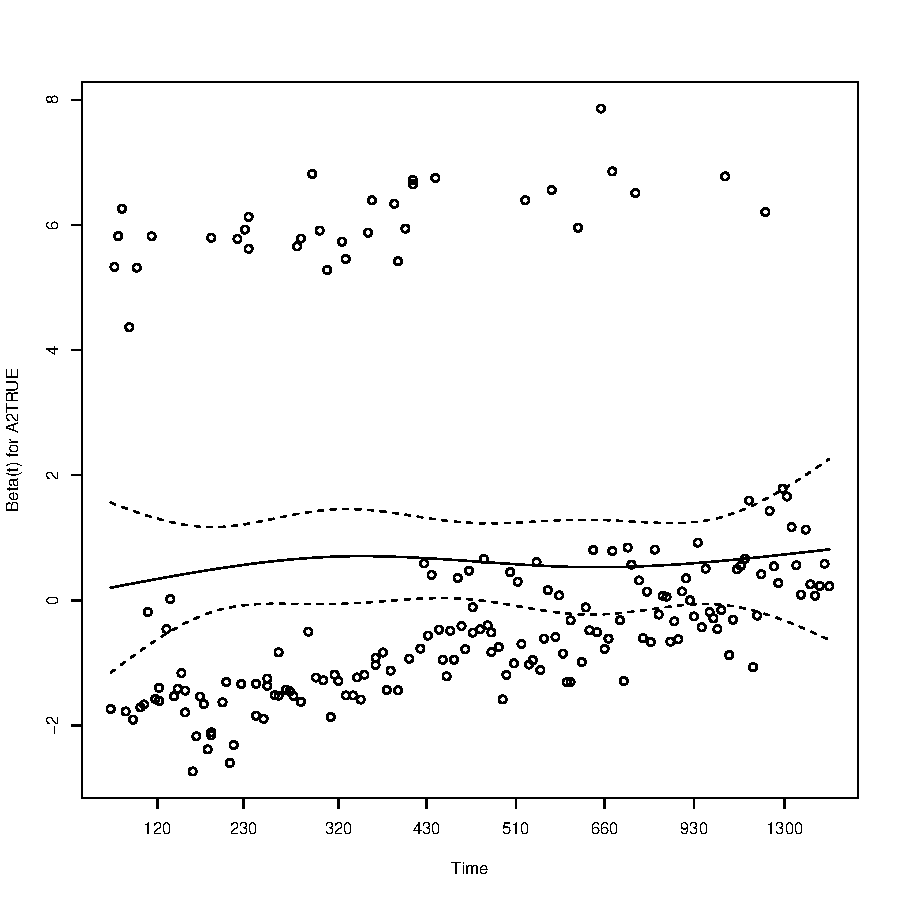
\includegraphics[width=\maxwidth]{figure/eda-ph-check-reduced-2} 

}




{\centering 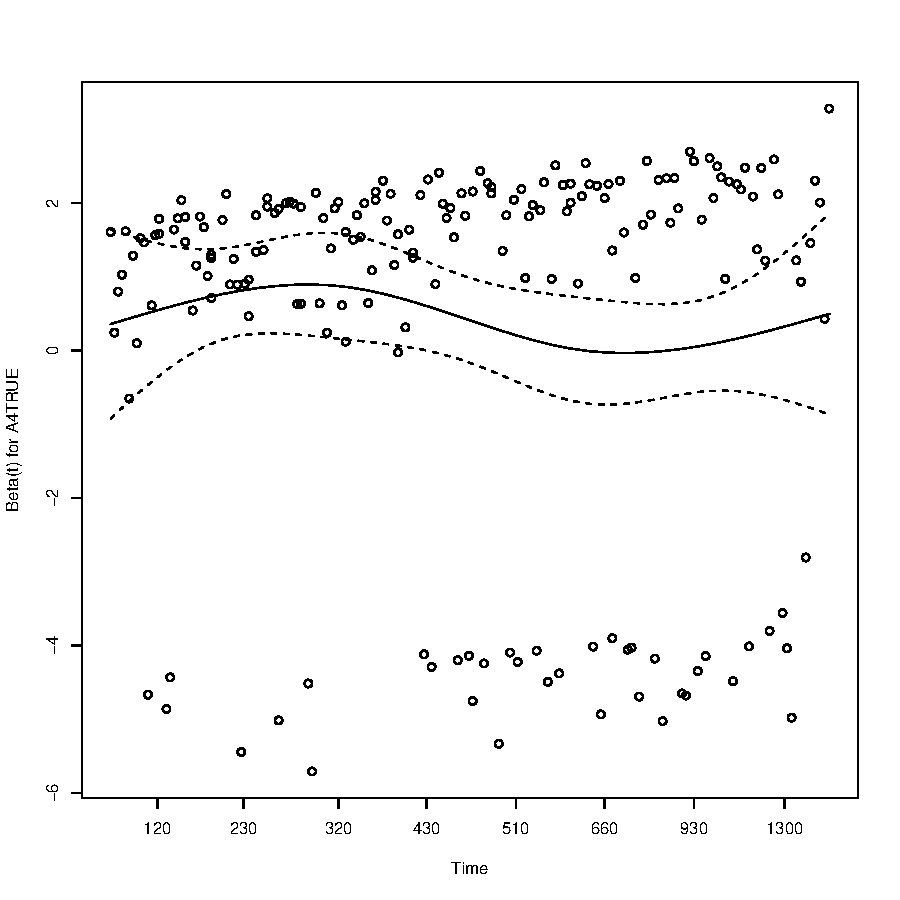
\includegraphics[width=\maxwidth]{figure/eda-ph-check-reduced-3} 

}



\end{knitrout}

\subsection{Outliers: reduced model}
\begin{knitrout}
\definecolor{shadecolor}{rgb}{0.969, 0.969, 0.969}\color{fgcolor}\begin{kframe}
\begin{alltt}
\hlkwd{plot}\hlstd{(}\hlkwd{resid}\hlstd{(fit.cph,} \hlkwc{type} \hlstd{=} \hlstr{"deviance"}\hlstd{))}
\end{alltt}
\end{kframe}

{\centering 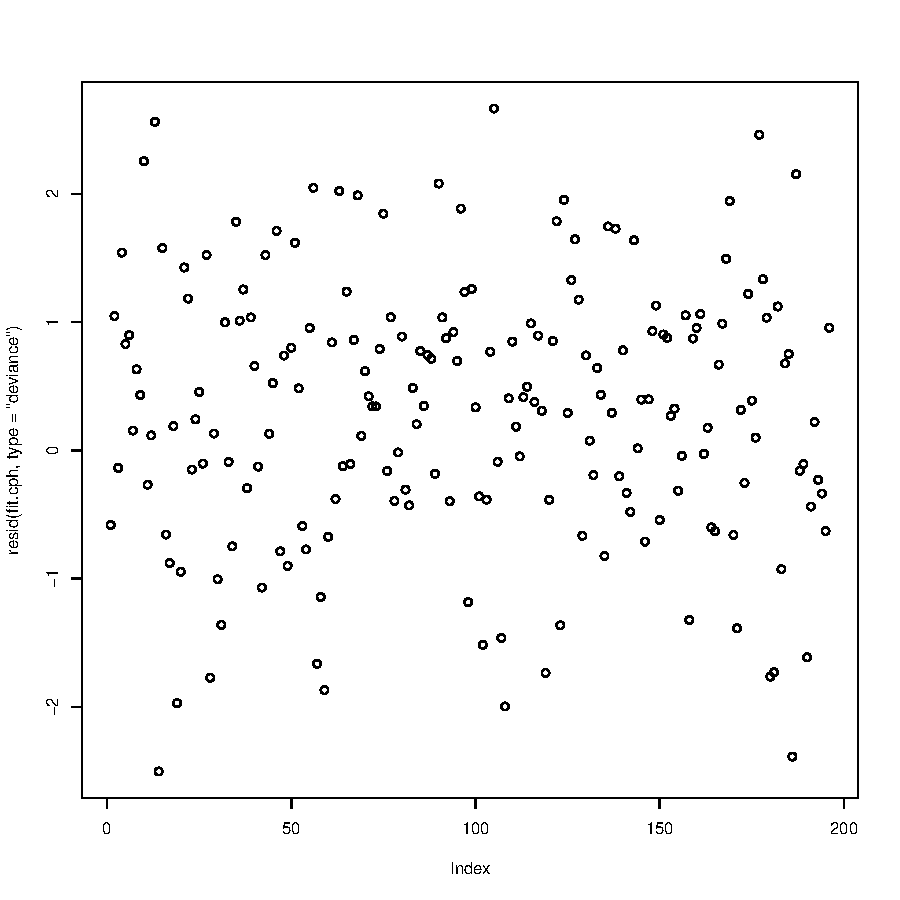
\includegraphics[width=\maxwidth]{figure/eda-outliers-reduced-1} 

}



\end{knitrout}

Now generate the restricted fit and examine the DFBETAS on the reduced model.

\begin{knitrout}
\definecolor{shadecolor}{rgb}{0.969, 0.969, 0.969}\color{fgcolor}\begin{kframe}
\begin{alltt}
\hlstd{temp} \hlkwb{=} \hlkwd{resid}\hlstd{(fit.cph,} \hlkwc{type} \hlstd{=} \hlstr{"dfbetas"}\hlstd{)}
\hlkwd{colnames}\hlstd{(temp)} \hlkwb{=} \hlkwd{names}\hlstd{(fit.cph}\hlopt{$}\hlstd{coefficients)}
\hlstd{temp} \hlkwb{=} \hlkwd{melt}\hlstd{(temp)}
\hlkwd{colnames}\hlstd{(temp)} \hlkwb{=} \hlkwd{c}\hlstd{(}\hlstr{"Patient"}\hlstd{,} \hlstr{"Coefficient"}\hlstd{,} \hlstr{"dfbetas"}\hlstd{)}
\hlnum{2}\hlopt{/}\hlkwd{sqrt}\hlstd{(}\hlkwd{nrow}\hlstd{(data))}  \hlcom{# The classic threshold for concern is 2/sqrt(n).}
\end{alltt}
\begin{verbatim}
## [1] 0.1429
\end{verbatim}
\begin{alltt}
\hlkwd{ggplot}\hlstd{(temp,} \hlkwd{aes}\hlstd{(}\hlkwc{y} \hlstd{=} \hlkwd{abs}\hlstd{(dfbetas),} \hlkwc{x} \hlstd{= Patient,} \hlkwc{col} \hlstd{= Coefficient))} \hlopt{+} \hlkwd{geom_point}\hlstd{()} \hlopt{+}
    \hlkwd{geom_hline}\hlstd{(}\hlkwc{yintercept} \hlstd{=} \hlnum{2}\hlopt{/}\hlkwd{sqrt}\hlstd{(}\hlkwd{nrow}\hlstd{(data)))}
\end{alltt}
\end{kframe}

{\centering 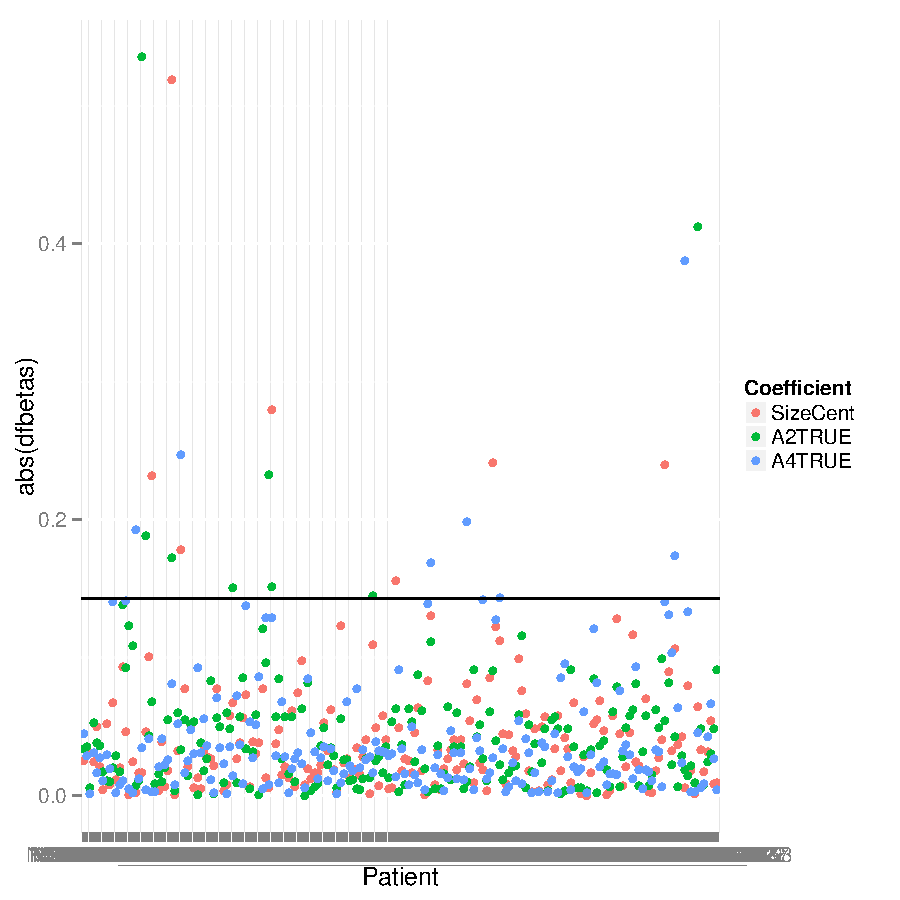
\includegraphics[width=\maxwidth]{figure/eda-dfbetas-reduced-1} 

}


\begin{kframe}\begin{alltt}
\hlkwd{sort}\hlstd{(}\hlkwd{apply}\hlstd{(}\hlkwd{abs}\hlstd{(}\hlkwd{resid}\hlstd{(fit.cph,} \hlkwc{type} \hlstd{=} \hlstr{"dfbetas"}\hlstd{)),} \hlnum{1}\hlstd{, max),} \hlkwc{decreasing} \hlstd{=} \hlnum{TRUE}\hlstd{)}
\end{alltt}
\begin{verbatim}
##  NSWPCN_144  NSWPCN_183 NSWPCN_1212 NSWPCN_1195  NSWPCN_318  NSWPCN_195 
##    0.535319    0.518522    0.412372    0.387309    0.279328    0.246925 
##  NSWPCN_799 NSWPCN_1182  NSWPCN_317  NSWPCN_154  NSWPCN_777  NSWPCN_142 
##    0.241159    0.239789    0.232758    0.231619    0.198560    0.192828 
##  NSWPCN_145 NSWPCN_1188  NSWPCN_655  NSWPCN_606  NSWPCN_296  NSWPCN_374 
##    0.188531    0.174002    0.168515    0.155810    0.150737    0.145092 
##  NSWPCN_802  NSWPCN_795  NSWPCN_133  NSWPCN_125  NSWPCN_654  NSWPCN_131 
##    0.143009    0.141584    0.141390    0.140472    0.138800    0.138044 
##  NSWPCN_307 NSWPCN_1196 NSWPCN_1186  NSWPCN_316 NSWPCN_1155  NSWPCN_801 
##    0.137409    0.132883    0.131227    0.128578    0.127761    0.127389 
##  NSWPCN_135  NSWPCN_354 NSWPCN_1143  NSWPCN_315 NSWPCN_1167  NSWPCN_814 
##    0.123283    0.123043    0.121087    0.120854    0.116675    0.115720 
##  NSWPCN_138 NSWPCN_1187  NSWPCN_152  NSWPCN_813 NSWPCN_1179  NSWPCN_333 
##    0.108794    0.103714    0.100222    0.099014    0.098728    0.097707 
## NSWPCN_1072 NSWPCN_1168  NSWPCN_269  NSWPCN_636 NSWPCN_1453 NSWPCN_1082 
##    0.095141    0.093522    0.092355    0.091215    0.090934    0.090854 
##  NSWPCN_789  NSWPCN_647  NSWPCN_312  NSWPCN_798 NSWPCN_1071  NSWPCN_305 
##    0.090769    0.087516    0.086378    0.085496    0.085364    0.085038 
##  NSWPCN_335  NSWPCN_322  NSWPCN_276 NSWPCN_1145  NSWPCN_364  NSWPCN_200 
##    0.084907    0.084847    0.083106    0.081794    0.077536    0.077276 
##  NSWPCN_281 NSWPCN_1157  NSWPCN_331  NSWPCN_303 NSWPCN_1172  NSWPCN_790 
##    0.077244    0.076161    0.074559    0.072324    0.070007    0.069602 
## NSWPCN_1146  NSWPCN_323  NSWPCN_360 NSWPCN_1088 NSWPCN_1222  NSWPCN_664 
##    0.068367    0.067802    0.067654    0.066832    0.066379    0.064549 
## NSWPCN_1189  NSWPCN_640  NSWPCN_351 NSWPCN_1177  NSWPCN_326  NSWPCN_651 
##    0.063748    0.062695    0.062145    0.061975    0.061638    0.061411 
## NSWPCN_1153 NSWPCN_1139  NSWPCN_284  NSWPCN_194  NSWPCN_769  NSWPCN_815 
##    0.060979    0.060563    0.059802    0.059695    0.059694    0.059379 
##  NSWPCN_310  NSWPCN_377 NSWPCN_1031 NSWPCN_1165  NSWPCN_294 NSWPCN_1029 
##    0.058826    0.057956    0.057888    0.057640    0.057463    0.057289 
## NSWPCN_1023  NSWPCN_320  NSWPCN_304  NSWPCN_324  NSWPCN_272  NSWPCN_182 
##    0.057254    0.057106    0.057097    0.056915    0.055722    0.055199 
## NSWPCN_1028  NSWPCN_781  NSWPCN_445  NSWPCN_268  NSWPCN_643  NSWPCN_308 
##    0.055045    0.053779    0.053775    0.053737    0.053434    0.053314 
##  NSWPCN_347   NSWPCN_10   NSWPCN_24  NSWPCN_257  NSWPCN_794 NSWPCN_1016 
##    0.053023    0.052498    0.052189    0.051883    0.051498    0.051284 
##   NSWPCN_13  NSWPCN_282 NSWPCN_1022 NSWPCN_1160  NSWPCN_375 NSWPCN_1178 
##    0.049613    0.049572    0.049531    0.048958    0.048914    0.048792 
## NSWPCN_1227 NSWPCN_1213 NSWPCN_1075 NSWPCN_1019 NSWPCN_1147  NSWPCN_665 
##    0.048631    0.048614    0.048561    0.048203    0.046858    0.046764 
##  NSWPCN_646  NSWPCN_336    NSWPCN_4  NSWPCN_804  NSWPCN_807 NSWPCN_1219 
##    0.045742    0.045469    0.045022    0.044914    0.043924    0.042407 
## NSWPCN_1190  NSWPCN_164  NSWPCN_666  NSWPCN_381  NSWPCN_770  NSWPCN_370 
##    0.042400    0.041379    0.040729    0.040591    0.040581    0.040421 
##  NSWPCN_309  NSWPCN_270  NSWPCN_637   NSWPCN_20  NSWPCN_273  NSWPCN_346 
##    0.038785    0.038276    0.036619    0.036126    0.035909    0.035845 
##  NSWPCN_657    NSWPCN_7 NSWPCN_1141  NSWPCN_369 NSWPCN_1158  NSWPCN_350 
##    0.035660    0.035272    0.033258    0.033176    0.032752    0.032716 
##  NSWPCN_376  NSWPCN_810  NSWPCN_341 NSWPCN_1171  NSWPCN_384  NSWPCN_126 
##    0.032695    0.032560    0.031861    0.031740    0.029033    0.028767 
##  NSWPCN_352  NSWPCN_811  NSWPCN_373  NSWPCN_638  NSWPCN_330  NSWPCN_358 
##    0.028581    0.028304    0.027879    0.026735    0.026383    0.025635 
##  NSWPCN_256  NSWPCN_283  NSWPCN_775  NSWPCN_166 NSWPCN_1170  NSWPCN_362 
##    0.024904    0.022669    0.022611    0.022181    0.021654    0.021446 
##  NSWPCN_280 NSWPCN_1207  NSWPCN_161  NSWPCN_656  NSWPCN_128  NSWPCN_366 
##    0.021341    0.021195    0.020940    0.020342    0.020270    0.019967 
##  NSWPCN_653  NSWPCN_363   NSWPCN_36  NSWPCN_662 NSWPCN_1136 NSWPCN_1150 
##    0.019505    0.019311    0.019303    0.019302    0.019072    0.018446 
## NSWPCN_1018 NSWPCN_1091 NSWPCN_1215 NSWPCN_1175   NSWPCN_21  NSWPCN_345 
##    0.017496    0.017407    0.016899    0.016870    0.016860    0.016454 
##  NSWPCN_143  NSWPCN_325 NSWPCN_1152  NSWPCN_658 NSWPCN_1176  NSWPCN_797 
##    0.016435    0.015767    0.015516    0.015427    0.015148    0.011796 
## NSWPCN_1211  NSWPCN_806  NSWPCN_157  NSWPCN_190  NSWPCN_334 NSWPCN_1027 
##    0.009221    0.008634    0.008317    0.008019    0.007766    0.007733 
##    NSWPCN_9  NSWPCN_353 NSWPCN_1140 NSWPCN_1020 
##    0.005630    0.005273    0.003534    0.003253
\end{verbatim}
\begin{alltt}
\hlkwd{sum}\hlstd{(}\hlkwd{apply}\hlstd{(}\hlkwd{abs}\hlstd{(}\hlkwd{resid}\hlstd{(fit.cph,} \hlkwc{type} \hlstd{=} \hlstr{"dfbetas"}\hlstd{)),} \hlnum{1}\hlstd{, max)} \hlopt{>} \hlnum{2}\hlopt{/}\hlkwd{sqrt}\hlstd{(}\hlkwd{nrow}\hlstd{(data)))}
\end{alltt}
\begin{verbatim}
## [1] 19
\end{verbatim}
\end{kframe}
\end{knitrout}

\subsection{Summary of EDA}
\begin{enumerate}
\item On the basis of pre-operative assessability and data availability, variables were filtered down to Sex, AgeCent, LocBody, SizeCent, A2, A4.
\item Functional forms for the continuous variates AgeCent and SizeCent indicated a possible slight quadratic effect on AgeCent, and a knee on SizeCent.  These were modelled by incorporating additional terms.
\item Analysis of a full model fit (with additional nonlinear terms included) indicated violation of PH for gender.  This was dealt with by stratification.  A slight PH violation by age was deemed unimportant. 
\item Variable selection by BIC (both stepwise and genetic all-subset) settled on a final model of Surv(Time,DSD) $\sim$ 1 + strata(SexM) + SizeCent + A2 + A4.  This model was refit by coxph. 
\item PH was verified on the final model.  Deviance residuals showed no egregious outliers. dfBetaS indicated a number of influential observations, which require checking.
\end{enumerate}

\section{Final fits}
\begin{knitrout}
\definecolor{shadecolor}{rgb}{0.969, 0.969, 0.969}\color{fgcolor}\begin{kframe}
\begin{alltt}
\hlstd{fit.cph} \hlkwb{=} \hlkwd{coxph}\hlstd{(}\hlkwd{Surv}\hlstd{(Time, DSD)} \hlopt{~} \hlkwd{strata}\hlstd{(SexM)} \hlopt{+} \hlstd{SizeCent} \hlopt{+} \hlstd{A2} \hlopt{+} \hlstd{A4,} \hlkwc{data} \hlstd{= data)}
\end{alltt}
\end{kframe}
\end{knitrout}

\begin{knitrout}
\definecolor{shadecolor}{rgb}{0.969, 0.969, 0.969}\color{fgcolor}\begin{kframe}
\begin{alltt}
\hlkwd{set.seed}\hlstd{(}\hlnum{20150111}\hlstd{)}
\hlstd{fit.rsf} \hlkwb{=} \hlkwd{rfsrc}\hlstd{(}\hlkwd{Surv}\hlstd{(Time, DSD)} \hlopt{~} \hlstd{SexM} \hlopt{+} \hlstd{AgeCent} \hlopt{+} \hlstd{LocBody} \hlopt{+} \hlstd{SizeCent} \hlopt{+} \hlstd{A2} \hlopt{+}
    \hlstd{A4,} \hlkwc{data} \hlstd{= data,} \hlkwc{mtry} \hlstd{=} \hlnum{1}\hlstd{,} \hlkwc{splitrule} \hlstd{=} \hlstr{"logrankscore"}\hlstd{,} \hlkwc{nsplit} \hlstd{=} \hlnum{2}\hlstd{,} \hlkwc{ntree} \hlstd{=} \hlnum{1000}\hlstd{)}
\end{alltt}
\end{kframe}
\end{knitrout}

\begin{knitrout}
\definecolor{shadecolor}{rgb}{0.969, 0.969, 0.969}\color{fgcolor}\begin{kframe}
\begin{alltt}
\hlstd{fit.gg} \hlkwb{=} \hlkwd{flexsurvreg}\hlstd{(}\hlkwd{Surv}\hlstd{(Time, DSD)} \hlopt{~} \hlstd{SexM} \hlopt{+} \hlstd{SizeCent} \hlopt{+} \hlstd{A2} \hlopt{+} \hlstd{A4,} \hlkwc{anc} \hlstd{=} \hlkwd{list}\hlstd{(}\hlkwc{sigma} \hlstd{=} \hlopt{~}\hlstd{SexM,}
    \hlkwc{Q} \hlstd{=} \hlopt{~}\hlstd{SexM),} \hlkwc{data} \hlstd{= data,} \hlkwc{dist} \hlstd{=} \hlstr{"gengamma"}\hlstd{)}

\hlstd{fit.gf} \hlkwb{=} \hlkwd{flexsurvreg}\hlstd{(}\hlkwd{Surv}\hlstd{(Time, DSD)} \hlopt{~} \hlstd{SexM} \hlopt{+} \hlstd{SizeCent} \hlopt{+} \hlstd{A2} \hlopt{+} \hlstd{A4,} \hlkwc{anc} \hlstd{=} \hlkwd{list}\hlstd{(}\hlkwc{sigma} \hlstd{=} \hlopt{~}\hlstd{SexM,}
    \hlkwc{Q} \hlstd{=} \hlopt{~}\hlstd{SexM,} \hlkwc{P} \hlstd{=} \hlopt{~}\hlstd{SexM),} \hlkwc{data} \hlstd{= data,} \hlkwc{dist} \hlstd{=} \hlstr{"genf"}\hlstd{)}

\hlstd{fit.gg}\hlopt{$}\hlstd{loglik}
\end{alltt}
\begin{verbatim}
## [1] -1355
\end{verbatim}
\begin{alltt}
\hlstd{fit.gf}\hlopt{$}\hlstd{loglik}
\end{alltt}
\begin{verbatim}
## [1] -1354
\end{verbatim}
\begin{alltt}
\hlkwd{pchisq}\hlstd{(}\hlnum{2} \hlopt{*} \hlstd{(fit.gf}\hlopt{$}\hlstd{loglik} \hlopt{-} \hlstd{fit.gg}\hlopt{$}\hlstd{loglik),} \hlnum{2}\hlstd{,} \hlkwc{lower.tail} \hlstd{=} \hlnum{FALSE}\hlstd{)}
\end{alltt}
\begin{verbatim}
## [1] 0.3371
\end{verbatim}
\begin{alltt}
\hlkwd{AIC}\hlstd{(fit.gg)}
\end{alltt}
\begin{verbatim}
## [1] 2727
\end{verbatim}
\begin{alltt}
\hlkwd{AIC}\hlstd{(fit.gf)}
\end{alltt}
\begin{verbatim}
## [1] 2729
\end{verbatim}
\begin{alltt}
\hlkwd{BIC}\hlstd{(fit.gg)}
\end{alltt}
\begin{verbatim}
## [1] 2757
\end{verbatim}
\begin{alltt}
\hlkwd{BIC}\hlstd{(fit.gf)}
\end{alltt}
\begin{verbatim}
## [1] 2765
\end{verbatim}
\begin{alltt}
\hlstd{fit.gg}
\end{alltt}
\begin{verbatim}
## 
## Call:
## flexsurvreg(formula = Surv(Time, DSD) ~ SexM + SizeCent + A2 +     A4, anc = list(sigma = ~SexM, Q = ~SexM), data = data, dist = "gengamma")
## 
## Estimates: 
##                  data mean  est       L95%      U95%      se      
## mu                     NA    6.41920   6.08210   6.75630   0.17199
## sigma                  NA    0.79193   0.68758   0.91211   0.05709
## Q                      NA    0.06489  -0.48729   0.61708   0.28173
## SexMTRUE          0.48469    0.36244   0.03548   0.68940   0.16682
## SizeCent          3.82143   -0.01028  -0.01751  -0.00305   0.00369
## A2TRUE            0.17347   -0.37995  -0.64171  -0.11818   0.13356
## A4TRUE            0.78061   -0.32171  -0.57137  -0.07206   0.12738
## sigma(SexMTRUE)   0.48469   -0.25903  -0.48789  -0.03017   0.11677
## Q(SexMTRUE)       0.48469    0.76270   0.04909   1.47631   0.36409
##                  exp(est)  L95%      U95%    
## mu                     NA        NA        NA
## sigma                  NA        NA        NA
## Q                      NA        NA        NA
## SexMTRUE          1.43683   1.03612   1.99251
## SizeCent          0.98977   0.98264   0.99695
## A2TRUE            0.68390   0.52639   0.88854
## A4TRUE            0.72491   0.56475   0.93048
## sigma(SexMTRUE)   0.77180   0.61392   0.97028
## Q(SexMTRUE)       2.14406   1.05032   4.37675
## 
## N = 196,  Events: 188,  Censored: 8
## Total time at risk: 113142
## Log-likelihood = -1355, df = 9
## AIC = 2727
\end{verbatim}
\end{kframe}
\end{knitrout}

\section{Fit assessment}
Plot fit stratified by sex, separate curves for A2, A4 status, at median (approx.) Size.
\begin{knitrout}
\definecolor{shadecolor}{rgb}{0.969, 0.969, 0.969}\color{fgcolor}\begin{kframe}
\begin{alltt}
\hlstd{temp.grid} \hlkwb{=} \hlkwd{expand.grid}\hlstd{(}\hlkwc{A4} \hlstd{=} \hlkwd{c}\hlstd{(}\hlnum{FALSE}\hlstd{,} \hlnum{TRUE}\hlstd{),} \hlkwc{A2} \hlstd{=} \hlkwd{c}\hlstd{(}\hlnum{FALSE}\hlstd{,} \hlnum{TRUE}\hlstd{),} \hlkwc{SexM} \hlstd{=} \hlkwd{c}\hlstd{(}\hlnum{FALSE}\hlstd{,}
    \hlnum{TRUE}\hlstd{),} \hlkwc{SizeCent} \hlstd{=} \hlnum{0}\hlstd{)}
\hlstd{temp.grid}\hlopt{$}\hlstd{ID} \hlkwb{=} \hlkwd{sprintf}\hlstd{(}\hlstr{"SexM=%s, A2=% -5s, A4=% -5s"}\hlstd{, temp.grid}\hlopt{$}\hlstd{SexM, temp.grid}\hlopt{$}\hlstd{A2,}
    \hlstd{temp.grid}\hlopt{$}\hlstd{A4)}
\hlstd{temp.preds} \hlkwb{=} \hlkwd{summary}\hlstd{(fit.gg,} \hlkwc{newdata} \hlstd{= temp.grid,} \hlkwc{type} \hlstd{=} \hlstr{"survival"}\hlstd{,} \hlkwc{t} \hlstd{=} \hlkwd{seq}\hlstd{(}\hlnum{0}\hlstd{,}
    \hlnum{365} \hlopt{*} \hlnum{5}\hlstd{,} \hlnum{30}\hlstd{))}
\hlstd{temp.preds2} \hlkwb{=} \hlkwd{do.call}\hlstd{(rbind, temp.preds)}
\hlstd{temp.preds2}\hlopt{$}\hlstd{group} \hlkwb{=} \hlkwd{rep}\hlstd{(}\hlkwd{gsub}\hlstd{(}\hlstr{".*ID="}\hlstd{,} \hlstr{""}\hlstd{,} \hlkwd{names}\hlstd{(temp.preds)),} \hlkwc{each} \hlstd{=} \hlkwd{nrow}\hlstd{(temp.preds[[}\hlnum{1}\hlstd{]]))}
\hlstd{temp.preds.cox} \hlkwb{=} \hlkwd{survfit}\hlstd{(fit.cph,} \hlkwc{newdata} \hlstd{= temp.grid)}

\hlstd{temp.survfit} \hlkwb{=} \hlkwd{survfit}\hlstd{(}\hlkwd{Surv}\hlstd{(Time, DSD)} \hlopt{~} \hlstd{SexM} \hlopt{+} \hlstd{A2} \hlopt{+} \hlstd{A4, data)}
\hlstd{temp.data} \hlkwb{=} \hlkwd{data.frame}\hlstd{(}\hlkwc{time} \hlstd{= temp.survfit}\hlopt{$}\hlstd{time,} \hlkwc{surv} \hlstd{= temp.survfit}\hlopt{$}\hlstd{surv,} \hlkwc{upper} \hlstd{= temp.survfit}\hlopt{$}\hlstd{lower,}
    \hlkwc{lower} \hlstd{= temp.survfit}\hlopt{$}\hlstd{upper,} \hlkwc{group} \hlstd{=} \hlkwd{rep}\hlstd{(}\hlkwd{names}\hlstd{(temp.survfit}\hlopt{$}\hlstd{strata), temp.survfit}\hlopt{$}\hlstd{strata),}
    \hlkwc{model} \hlstd{=} \hlstr{"KM"}\hlstd{)}
\hlstd{temp.data} \hlkwb{=} \hlkwd{rbind}\hlstd{(temp.data,} \hlkwd{data.frame}\hlstd{(}\hlkwc{time} \hlstd{= temp.preds2}\hlopt{$}\hlstd{time,} \hlkwc{surv} \hlstd{= temp.preds2}\hlopt{$}\hlstd{est,}
    \hlkwc{upper} \hlstd{= temp.preds2}\hlopt{$}\hlstd{ucl,} \hlkwc{lower} \hlstd{= temp.preds2}\hlopt{$}\hlstd{lcl,} \hlkwc{group} \hlstd{= temp.preds2}\hlopt{$}\hlstd{group,}
    \hlkwc{model} \hlstd{=} \hlstr{"GG"}\hlstd{))}
\hlstd{temp.data} \hlkwb{=} \hlkwd{rbind}\hlstd{(temp.data,} \hlkwd{data.frame}\hlstd{(}\hlkwc{time} \hlstd{= temp.preds.cox}\hlopt{$}\hlstd{time,} \hlkwc{surv} \hlstd{= temp.preds.cox}\hlopt{$}\hlstd{surv,}
    \hlkwc{upper} \hlstd{= temp.preds.cox}\hlopt{$}\hlstd{upper,} \hlkwc{lower} \hlstd{= temp.preds.cox}\hlopt{$}\hlstd{lower,} \hlkwc{group} \hlstd{=} \hlkwd{rep}\hlstd{(temp.grid}\hlopt{$}\hlstd{ID,}
        \hlstd{temp.preds.cox}\hlopt{$}\hlstd{strata),} \hlkwc{model} \hlstd{=} \hlstr{"CPH"}\hlstd{))}
\hlstd{temp.data}\hlopt{$}\hlstd{Sex} \hlkwb{=} \hlkwd{c}\hlstd{(}\hlstr{"Male"}\hlstd{,} \hlstr{"Female"}\hlstd{)[}\hlkwd{grepl}\hlstd{(}\hlstr{"SexM=FALSE"}\hlstd{, temp.data}\hlopt{$}\hlstd{group)} \hlopt{+} \hlnum{1}\hlstd{]}
\hlstd{temp.data}\hlopt{$}\hlstd{A2} \hlkwb{=} \hlkwd{c}\hlstd{(}\hlstr{"A2-"}\hlstd{,} \hlstr{"A2+"}\hlstd{)[}\hlkwd{grepl}\hlstd{(}\hlstr{"A2=TRUE"}\hlstd{, temp.data}\hlopt{$}\hlstd{group)} \hlopt{+} \hlnum{1}\hlstd{]}
\hlstd{temp.data}\hlopt{$}\hlstd{A4} \hlkwb{=} \hlkwd{c}\hlstd{(}\hlstr{"A4-"}\hlstd{,} \hlstr{"A4+"}\hlstd{)[}\hlkwd{grepl}\hlstd{(}\hlstr{"A4=TRUE"}\hlstd{, temp.data}\hlopt{$}\hlstd{group)} \hlopt{+} \hlnum{1}\hlstd{]}

\hlkwd{ggplot}\hlstd{(temp.data,} \hlkwd{aes}\hlstd{(}\hlkwc{x} \hlstd{=} \hlkwd{log}\hlstd{(time),} \hlkwc{y} \hlstd{=} \hlkwd{log}\hlstd{(}\hlopt{-}\hlkwd{log}\hlstd{(surv)),} \hlkwc{ymin} \hlstd{=} \hlkwd{log}\hlstd{(}\hlopt{-}\hlkwd{log}\hlstd{(lower)),}
    \hlkwc{ymax} \hlstd{=} \hlkwd{log}\hlstd{(}\hlopt{-}\hlkwd{log}\hlstd{(upper)),} \hlkwc{colour} \hlstd{= model,} \hlkwc{fill} \hlstd{= model))} \hlopt{+} \hlkwd{geom_ribbon}\hlstd{(}\hlkwc{alpha} \hlstd{=} \hlnum{0.25}\hlstd{,}
    \hlkwc{colour} \hlstd{=} \hlnum{NA}\hlstd{)} \hlopt{+} \hlkwd{geom_line}\hlstd{()} \hlopt{+} \hlkwd{xlim}\hlstd{(}\hlnum{4}\hlstd{,} \hlnum{7}\hlstd{)} \hlopt{+} \hlkwd{ylim}\hlstd{(}\hlopt{-}\hlnum{4}\hlstd{,} \hlnum{2}\hlstd{)} \hlopt{+} \hlkwd{facet_grid}\hlstd{(A2} \hlopt{~}
    \hlstd{A4} \hlopt{~} \hlstd{Sex)}
\end{alltt}


{\ttfamily\noindent\color{warningcolor}{\#\# Warning: Removed 46 rows containing missing values (geom\_path).}}

{\ttfamily\noindent\color{warningcolor}{\#\# Warning: Removed 41 rows containing missing values (geom\_path).}}

{\ttfamily\noindent\color{warningcolor}{\#\# Warning: Removed 48 rows containing missing values (geom\_path).}}

{\ttfamily\noindent\color{warningcolor}{\#\# Warning: Removed 44 rows containing missing values (geom\_path).}}

{\ttfamily\noindent\color{warningcolor}{\#\# Warning: Removed 39 rows containing missing values (geom\_path).}}

{\ttfamily\noindent\color{warningcolor}{\#\# Warning: Removed 37 rows containing missing values (geom\_path).}}

{\ttfamily\noindent\color{warningcolor}{\#\# Warning: Removed 40 rows containing missing values (geom\_path).}}

{\ttfamily\noindent\color{warningcolor}{\#\# Warning: Removed 38 rows containing missing values (geom\_path).}}\end{kframe}

{\centering 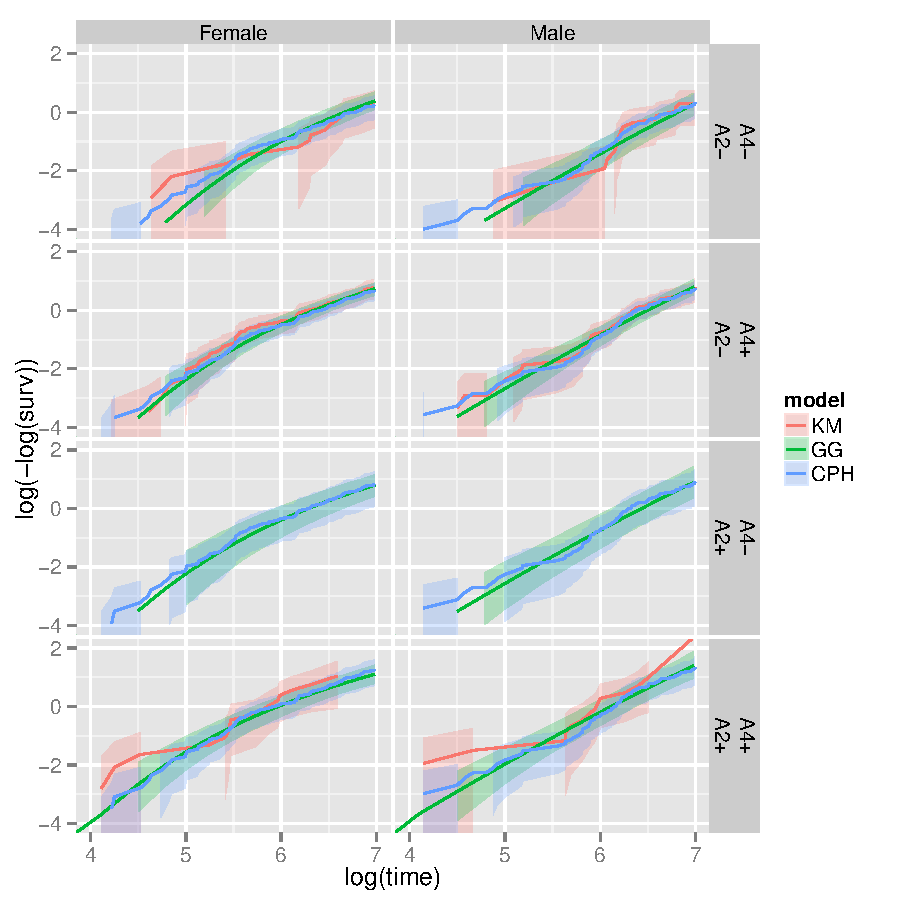
\includegraphics[width=\maxwidth]{figure/final-fit-assessment-1} 

}


\begin{kframe}\begin{alltt}
\hlkwd{ggplot}\hlstd{(temp.data,} \hlkwd{aes}\hlstd{(}\hlkwc{x} \hlstd{= time,} \hlkwc{y} \hlstd{= surv,} \hlkwc{ymin} \hlstd{= lower,} \hlkwc{ymax} \hlstd{= upper,} \hlkwc{colour} \hlstd{= model,}
    \hlkwc{fill} \hlstd{= model))} \hlopt{+} \hlkwd{geom_ribbon}\hlstd{(}\hlkwc{alpha} \hlstd{=} \hlnum{0.25}\hlstd{,} \hlkwc{colour} \hlstd{=} \hlnum{NA}\hlstd{)} \hlopt{+} \hlkwd{geom_line}\hlstd{()} \hlopt{+}
    \hlkwd{xlim}\hlstd{(}\hlnum{0}\hlstd{,} \hlnum{2000}\hlstd{)} \hlopt{+} \hlkwd{ylim}\hlstd{(}\hlnum{0}\hlstd{,} \hlnum{1}\hlstd{)} \hlopt{+} \hlkwd{facet_grid}\hlstd{(A2} \hlopt{~} \hlstd{A4} \hlopt{~} \hlstd{Sex)}
\end{alltt}


{\ttfamily\noindent\color{warningcolor}{\#\# Warning: Removed 3 rows containing missing values (geom\_path).}}

{\ttfamily\noindent\color{warningcolor}{\#\# Warning: Removed 3 rows containing missing values (geom\_path).}}

{\ttfamily\noindent\color{warningcolor}{\#\# Warning: Removed 2 rows containing missing values (geom\_path).}}

{\ttfamily\noindent\color{warningcolor}{\#\# Warning: Removed 2 rows containing missing values (geom\_path).}}\end{kframe}

{\centering 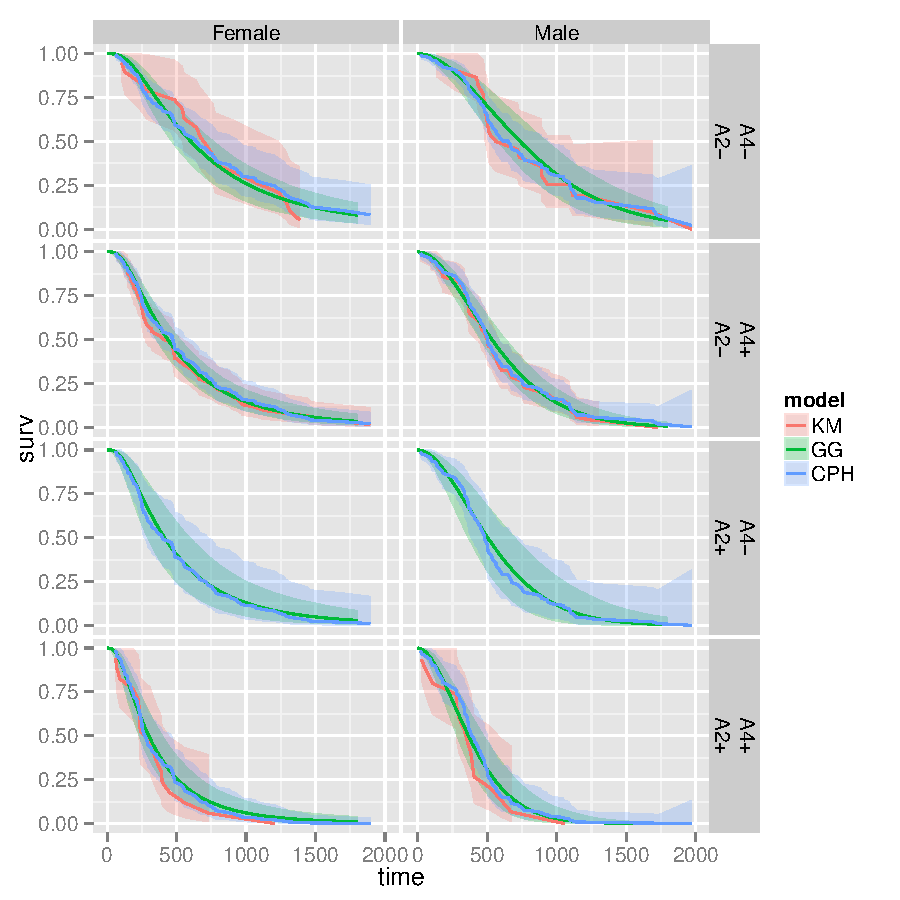
\includegraphics[width=\maxwidth]{figure/final-fit-assessment-2} 

}



\end{knitrout}

Some deviation though not significant.  Most concerning is the A2- A4- female group, survival of which is underestimated by the flexsurv model.  To approach this in a modelling sense would require interaction terms between Sex and A2, A4. Overfitting seems likely considering the very few data available for the A2+/A4- group.  Perhaps just add a single "DoubleNegFemale" term.
\begin{knitrout}
\definecolor{shadecolor}{rgb}{0.969, 0.969, 0.969}\color{fgcolor}\begin{kframe}
\begin{alltt}
\hlstd{fit.gg2} \hlkwb{=} \hlkwd{flexsurvreg}\hlstd{(}\hlkwd{Surv}\hlstd{(Time, DSD)} \hlopt{~} \hlstd{SexM} \hlopt{+} \hlstd{SizeCent} \hlopt{+} \hlstd{A2} \hlopt{+} \hlstd{A4} \hlopt{+} \hlkwd{I}\hlstd{(SexM} \hlopt{==}
    \hlnum{FALSE} \hlopt{&} \hlstd{A2} \hlopt{==} \hlnum{FALSE} \hlopt{&} \hlstd{A4} \hlopt{==} \hlnum{FALSE}\hlstd{),} \hlkwc{anc} \hlstd{=} \hlkwd{list}\hlstd{(}\hlkwc{sigma} \hlstd{=} \hlopt{~}\hlstd{SexM,} \hlkwc{Q} \hlstd{=} \hlopt{~}\hlstd{SexM),}
    \hlkwc{data} \hlstd{= data,} \hlkwc{dist} \hlstd{=} \hlstr{"gengamma"}\hlstd{)}

\hlkwd{AIC}\hlstd{(fit.gg)}
\end{alltt}
\begin{verbatim}
## [1] 2727
\end{verbatim}
\begin{alltt}
\hlkwd{AIC}\hlstd{(fit.gg2)}
\end{alltt}
\begin{verbatim}
## [1] 2729
\end{verbatim}
\begin{alltt}
\hlkwd{AIC}\hlstd{(fit.gg)} \hlopt{-} \hlkwd{AIC}\hlstd{(fit.gg2)}
\end{alltt}
\begin{verbatim}
## [1] -1.604
\end{verbatim}
\begin{alltt}
\hlcom{# Equivocal on AIC.  BIC would favour gg then.}

\hlkwd{pchisq}\hlstd{(}\hlopt{-}\hlnum{2} \hlopt{*} \hlstd{(fit.gg}\hlopt{$}\hlstd{loglik} \hlopt{-} \hlstd{fit.gg2}\hlopt{$}\hlstd{loglik),} \hlnum{1}\hlstd{,} \hlkwc{lower.tail} \hlstd{=} \hlnum{FALSE}\hlstd{)}
\end{alltt}
\begin{verbatim}
## [1] 0.5291
\end{verbatim}
\begin{alltt}
\hlcom{# Not good evidence on LRT}
\end{alltt}
\end{kframe}
\end{knitrout}

See how it plots relative to the others.
\begin{knitrout}
\definecolor{shadecolor}{rgb}{0.969, 0.969, 0.969}\color{fgcolor}\begin{kframe}
\begin{alltt}
\hlstd{temp.preds} \hlkwb{=} \hlkwd{summary}\hlstd{(fit.gg2,} \hlkwc{newdata} \hlstd{= temp.grid,} \hlkwc{type} \hlstd{=} \hlstr{"survival"}\hlstd{,} \hlkwc{t} \hlstd{=} \hlkwd{seq}\hlstd{(}\hlnum{0}\hlstd{,}
    \hlnum{365} \hlopt{*} \hlnum{5}\hlstd{,} \hlnum{30}\hlstd{))}
\hlstd{temp.preds2} \hlkwb{=} \hlkwd{do.call}\hlstd{(rbind, temp.preds)}
\hlstd{temp.preds2}\hlopt{$}\hlstd{group} \hlkwb{=} \hlkwd{rep}\hlstd{(}\hlkwd{gsub}\hlstd{(}\hlstr{".*ID="}\hlstd{,} \hlstr{""}\hlstd{,} \hlkwd{names}\hlstd{(temp.preds)),} \hlkwc{each} \hlstd{=} \hlkwd{nrow}\hlstd{(temp.preds[[}\hlnum{1}\hlstd{]]))}
\hlstd{temp.data} \hlkwb{=} \hlkwd{rbind}\hlstd{(temp.data,} \hlkwd{data.frame}\hlstd{(}\hlkwc{time} \hlstd{= temp.preds2}\hlopt{$}\hlstd{time,} \hlkwc{surv} \hlstd{= temp.preds2}\hlopt{$}\hlstd{est,}
    \hlkwc{upper} \hlstd{= temp.preds2}\hlopt{$}\hlstd{ucl,} \hlkwc{lower} \hlstd{= temp.preds2}\hlopt{$}\hlstd{lcl,} \hlkwc{group} \hlstd{= temp.preds2}\hlopt{$}\hlstd{group,}
    \hlkwc{model} \hlstd{=} \hlstr{"GG2"}\hlstd{,} \hlkwc{Sex} \hlstd{=} \hlnum{NA}\hlstd{,} \hlkwc{A2} \hlstd{=} \hlnum{NA}\hlstd{,} \hlkwc{A4} \hlstd{=} \hlnum{NA}\hlstd{))}
\hlstd{temp.data}\hlopt{$}\hlstd{Sex} \hlkwb{=} \hlkwd{c}\hlstd{(}\hlstr{"Male"}\hlstd{,} \hlstr{"Female"}\hlstd{)[}\hlkwd{grepl}\hlstd{(}\hlstr{"SexM=FALSE"}\hlstd{, temp.data}\hlopt{$}\hlstd{group)} \hlopt{+} \hlnum{1}\hlstd{]}
\hlstd{temp.data}\hlopt{$}\hlstd{A2} \hlkwb{=} \hlkwd{c}\hlstd{(}\hlstr{"A2-"}\hlstd{,} \hlstr{"A2+"}\hlstd{)[}\hlkwd{grepl}\hlstd{(}\hlstr{"A2=TRUE"}\hlstd{, temp.data}\hlopt{$}\hlstd{group)} \hlopt{+} \hlnum{1}\hlstd{]}
\hlstd{temp.data}\hlopt{$}\hlstd{A4} \hlkwb{=} \hlkwd{c}\hlstd{(}\hlstr{"A4-"}\hlstd{,} \hlstr{"A4+"}\hlstd{)[}\hlkwd{grepl}\hlstd{(}\hlstr{"A4=TRUE"}\hlstd{, temp.data}\hlopt{$}\hlstd{group)} \hlopt{+} \hlnum{1}\hlstd{]}

\hlkwd{ggplot}\hlstd{(temp.data,} \hlkwd{aes}\hlstd{(}\hlkwc{x} \hlstd{=} \hlkwd{log}\hlstd{(time),} \hlkwc{y} \hlstd{=} \hlkwd{log}\hlstd{(}\hlopt{-}\hlkwd{log}\hlstd{(surv)),} \hlkwc{ymin} \hlstd{=} \hlkwd{log}\hlstd{(}\hlopt{-}\hlkwd{log}\hlstd{(lower)),}
    \hlkwc{ymax} \hlstd{=} \hlkwd{log}\hlstd{(}\hlopt{-}\hlkwd{log}\hlstd{(upper)),} \hlkwc{colour} \hlstd{= model,} \hlkwc{fill} \hlstd{= model))} \hlopt{+} \hlkwd{geom_ribbon}\hlstd{(}\hlkwc{alpha} \hlstd{=} \hlnum{0.25}\hlstd{,}
    \hlkwc{colour} \hlstd{=} \hlnum{NA}\hlstd{)} \hlopt{+} \hlkwd{geom_line}\hlstd{()} \hlopt{+} \hlkwd{xlim}\hlstd{(}\hlnum{4}\hlstd{,} \hlnum{7}\hlstd{)} \hlopt{+} \hlkwd{ylim}\hlstd{(}\hlopt{-}\hlnum{4}\hlstd{,} \hlnum{2}\hlstd{)} \hlopt{+} \hlkwd{facet_grid}\hlstd{(A2} \hlopt{~}
    \hlstd{A4} \hlopt{~} \hlstd{Sex)}
\end{alltt}


{\ttfamily\noindent\color{warningcolor}{\#\# Warning: Removed 71 rows containing missing values (geom\_path).}}

{\ttfamily\noindent\color{warningcolor}{\#\# Warning: Removed 66 rows containing missing values (geom\_path).}}

{\ttfamily\noindent\color{warningcolor}{\#\# Warning: Removed 73 rows containing missing values (geom\_path).}}

{\ttfamily\noindent\color{warningcolor}{\#\# Warning: Removed 69 rows containing missing values (geom\_path).}}

{\ttfamily\noindent\color{warningcolor}{\#\# Warning: Removed 64 rows containing missing values (geom\_path).}}

{\ttfamily\noindent\color{warningcolor}{\#\# Warning: Removed 62 rows containing missing values (geom\_path).}}

{\ttfamily\noindent\color{warningcolor}{\#\# Warning: Removed 65 rows containing missing values (geom\_path).}}

{\ttfamily\noindent\color{warningcolor}{\#\# Warning: Removed 63 rows containing missing values (geom\_path).}}\end{kframe}

{\centering 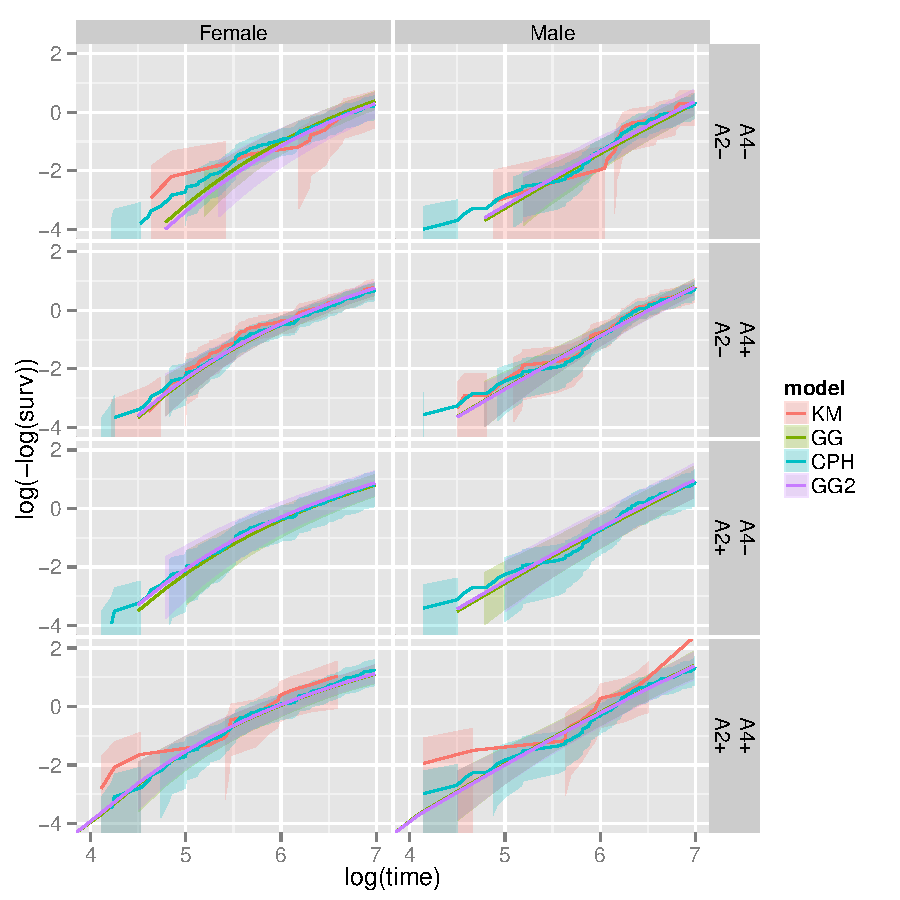
\includegraphics[width=\maxwidth]{figure/final-fit-assessment-2-1} 

}


\begin{kframe}\begin{alltt}
\hlkwd{ggplot}\hlstd{(temp.data,} \hlkwd{aes}\hlstd{(}\hlkwc{x} \hlstd{= time,} \hlkwc{y} \hlstd{= surv,} \hlkwc{ymin} \hlstd{= lower,} \hlkwc{ymax} \hlstd{= upper,} \hlkwc{colour} \hlstd{= model,}
    \hlkwc{fill} \hlstd{= model))} \hlopt{+} \hlkwd{geom_ribbon}\hlstd{(}\hlkwc{alpha} \hlstd{=} \hlnum{0.25}\hlstd{,} \hlkwc{colour} \hlstd{=} \hlnum{NA}\hlstd{)} \hlopt{+} \hlkwd{geom_line}\hlstd{()} \hlopt{+}
    \hlkwd{xlim}\hlstd{(}\hlnum{0}\hlstd{,} \hlnum{2000}\hlstd{)} \hlopt{+} \hlkwd{ylim}\hlstd{(}\hlnum{0}\hlstd{,} \hlnum{1}\hlstd{)} \hlopt{+} \hlkwd{facet_grid}\hlstd{(A2} \hlopt{~} \hlstd{A4} \hlopt{~} \hlstd{Sex)}
\end{alltt}


{\ttfamily\noindent\color{warningcolor}{\#\# Warning: Removed 3 rows containing missing values (geom\_path).}}

{\ttfamily\noindent\color{warningcolor}{\#\# Warning: Removed 3 rows containing missing values (geom\_path).}}

{\ttfamily\noindent\color{warningcolor}{\#\# Warning: Removed 2 rows containing missing values (geom\_path).}}

{\ttfamily\noindent\color{warningcolor}{\#\# Warning: Removed 2 rows containing missing values (geom\_path).}}\end{kframe}

{\centering 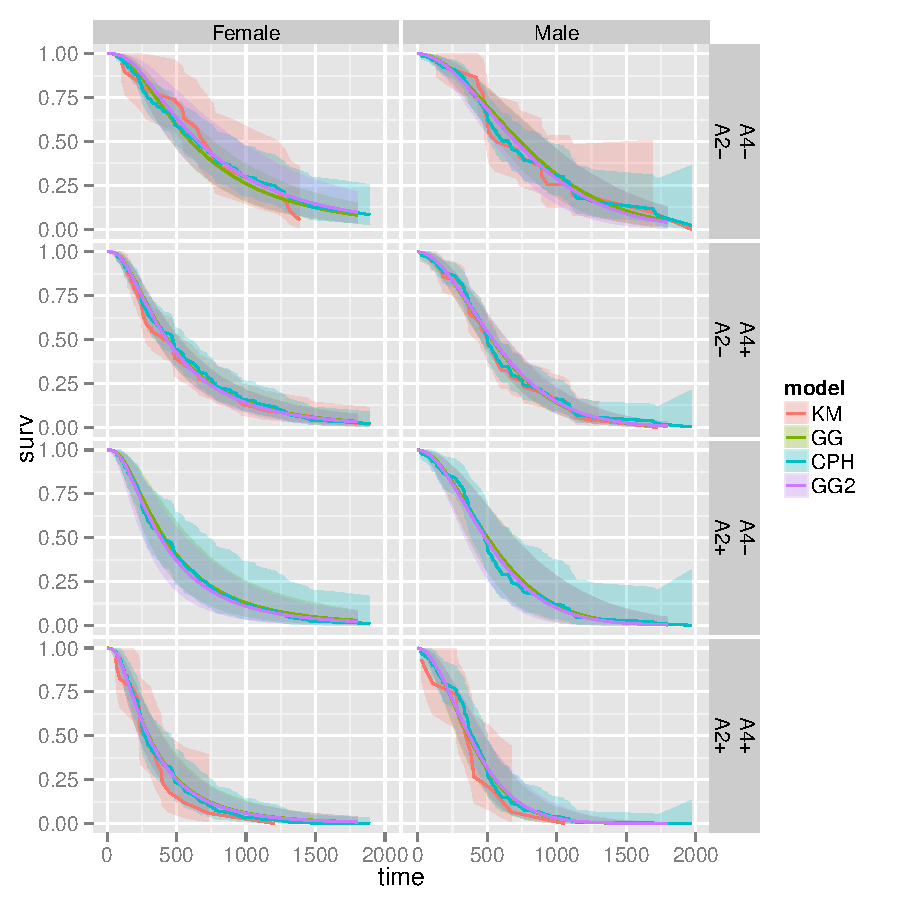
\includegraphics[width=\maxwidth]{figure/final-fit-assessment-2-2} 

}



\end{knitrout}

An alternative take, showing errors with the KMs only.
\begin{knitrout}
\definecolor{shadecolor}{rgb}{0.969, 0.969, 0.969}\color{fgcolor}\begin{kframe}
\begin{alltt}
\hlstd{temp.data}\hlopt{$}\hlstd{lower[temp.data}\hlopt{$}\hlstd{model} \hlopt{!=} \hlstr{"KM"}\hlstd{]} \hlkwb{=} \hlnum{NA}
\hlstd{temp.data}\hlopt{$}\hlstd{upper[temp.data}\hlopt{$}\hlstd{model} \hlopt{!=} \hlstr{"KM"}\hlstd{]} \hlkwb{=} \hlnum{NA}
\hlkwd{ggplot}\hlstd{(temp.data,} \hlkwd{aes}\hlstd{(}\hlkwc{x} \hlstd{=} \hlkwd{log}\hlstd{(time),} \hlkwc{y} \hlstd{=} \hlkwd{log}\hlstd{(}\hlopt{-}\hlkwd{log}\hlstd{(surv)),} \hlkwc{ymin} \hlstd{=} \hlkwd{log}\hlstd{(}\hlopt{-}\hlkwd{log}\hlstd{(lower)),}
    \hlkwc{ymax} \hlstd{=} \hlkwd{log}\hlstd{(}\hlopt{-}\hlkwd{log}\hlstd{(upper)),} \hlkwc{colour} \hlstd{= model,} \hlkwc{fill} \hlstd{= model))} \hlopt{+} \hlkwd{geom_ribbon}\hlstd{(}\hlkwc{alpha} \hlstd{=} \hlnum{0.25}\hlstd{,}
    \hlkwc{colour} \hlstd{=} \hlnum{NA}\hlstd{)} \hlopt{+} \hlkwd{geom_line}\hlstd{()} \hlopt{+} \hlkwd{xlim}\hlstd{(}\hlnum{4}\hlstd{,} \hlnum{7}\hlstd{)} \hlopt{+} \hlkwd{ylim}\hlstd{(}\hlopt{-}\hlnum{4}\hlstd{,} \hlnum{2}\hlstd{)} \hlopt{+} \hlkwd{facet_grid}\hlstd{(A2} \hlopt{~}
    \hlstd{A4} \hlopt{~} \hlstd{Sex)}
\end{alltt}


{\ttfamily\noindent\color{warningcolor}{\#\# Warning: Removed 71 rows containing missing values (geom\_path).}}

{\ttfamily\noindent\color{warningcolor}{\#\# Warning: Removed 66 rows containing missing values (geom\_path).}}

{\ttfamily\noindent\color{warningcolor}{\#\# Warning: Removed 73 rows containing missing values (geom\_path).}}

{\ttfamily\noindent\color{warningcolor}{\#\# Warning: Removed 69 rows containing missing values (geom\_path).}}

{\ttfamily\noindent\color{warningcolor}{\#\# Warning: Removed 64 rows containing missing values (geom\_path).}}

{\ttfamily\noindent\color{warningcolor}{\#\# Warning: Removed 62 rows containing missing values (geom\_path).}}

{\ttfamily\noindent\color{warningcolor}{\#\# Warning: Removed 65 rows containing missing values (geom\_path).}}

{\ttfamily\noindent\color{warningcolor}{\#\# Warning: Removed 63 rows containing missing values (geom\_path).}}\end{kframe}

{\centering 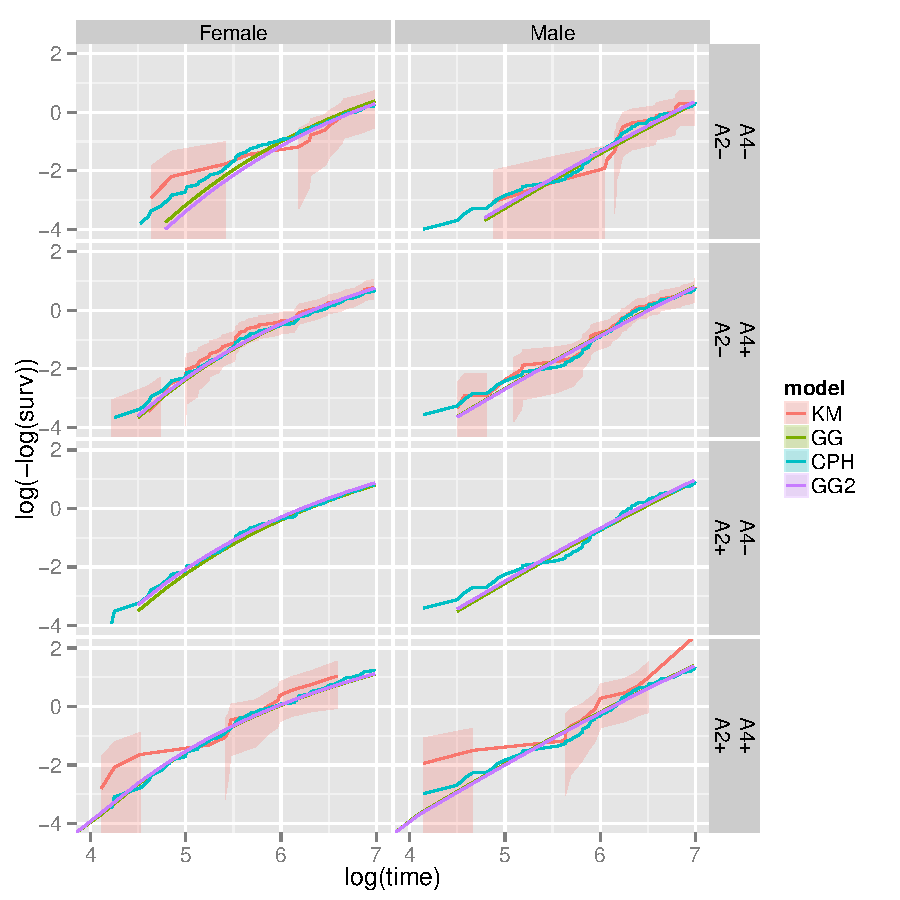
\includegraphics[width=\maxwidth]{figure/final-fit-assessment-3-1} 

}


\begin{kframe}\begin{alltt}
\hlkwd{ggplot}\hlstd{(temp.data,} \hlkwd{aes}\hlstd{(}\hlkwc{x} \hlstd{= time,} \hlkwc{y} \hlstd{= surv,} \hlkwc{ymin} \hlstd{= lower,} \hlkwc{ymax} \hlstd{= upper,} \hlkwc{colour} \hlstd{= model,}
    \hlkwc{fill} \hlstd{= model))} \hlopt{+} \hlkwd{geom_ribbon}\hlstd{(}\hlkwc{alpha} \hlstd{=} \hlnum{0.25}\hlstd{,} \hlkwc{colour} \hlstd{=} \hlnum{NA}\hlstd{)} \hlopt{+} \hlkwd{geom_line}\hlstd{()} \hlopt{+}
    \hlkwd{xlim}\hlstd{(}\hlnum{0}\hlstd{,} \hlnum{2000}\hlstd{)} \hlopt{+} \hlkwd{ylim}\hlstd{(}\hlnum{0}\hlstd{,} \hlnum{1}\hlstd{)} \hlopt{+} \hlkwd{facet_grid}\hlstd{(A2} \hlopt{~} \hlstd{A4} \hlopt{~} \hlstd{Sex)}
\end{alltt}


{\ttfamily\noindent\color{warningcolor}{\#\# Warning: Removed 3 rows containing missing values (geom\_path).}}

{\ttfamily\noindent\color{warningcolor}{\#\# Warning: Removed 3 rows containing missing values (geom\_path).}}

{\ttfamily\noindent\color{warningcolor}{\#\# Warning: Removed 2 rows containing missing values (geom\_path).}}

{\ttfamily\noindent\color{warningcolor}{\#\# Warning: Removed 2 rows containing missing values (geom\_path).}}\end{kframe}

{\centering 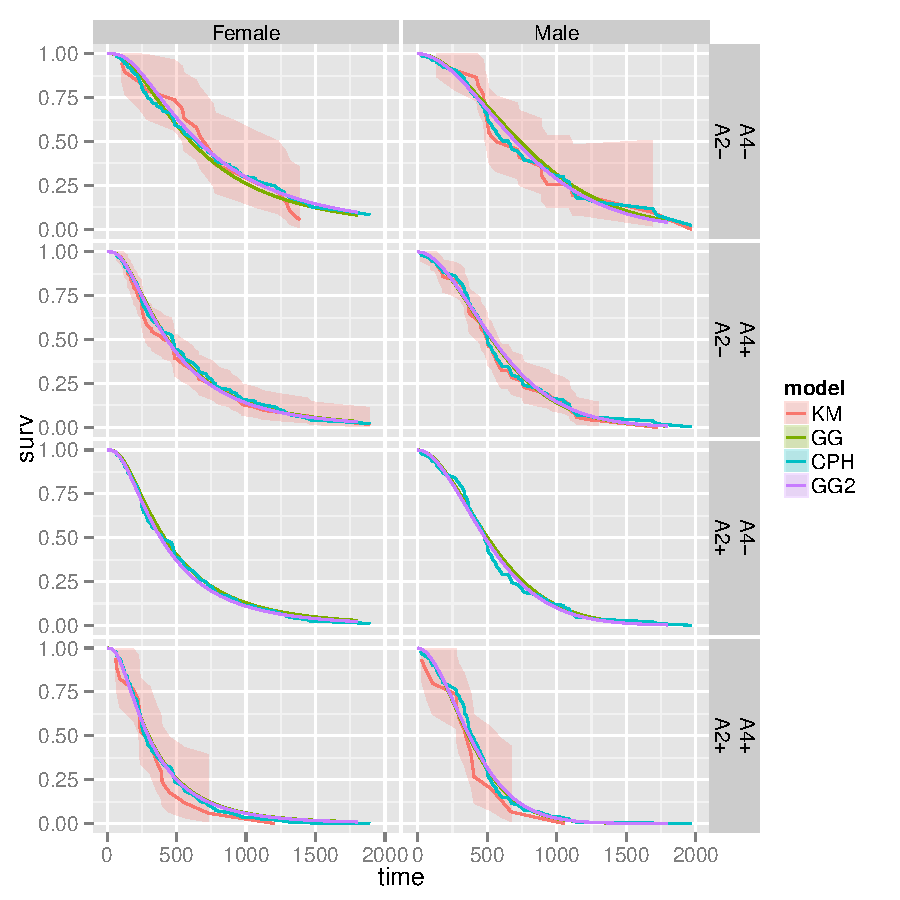
\includegraphics[width=\maxwidth]{figure/final-fit-assessment-3-2} 

}



\end{knitrout}

\section{Model selection}
It looks like that's as far as we can go with tweaking the fits.  Time to put the different models against each other on the holdout data, and choose a winner.

DIY IBS, wooo.
\begin{knitrout}
\definecolor{shadecolor}{rgb}{0.969, 0.969, 0.969}\color{fgcolor}\begin{kframe}
\begin{alltt}
\hlstd{calcIBS} \hlkwb{=} \hlkwa{function}\hlstd{(}\hlkwc{surv}\hlstd{,} \hlkwc{pred}\hlstd{,} \hlkwc{pred_times}\hlstd{,} \hlkwc{max_time}\hlstd{) \{}
    \hlkwd{stopifnot}\hlstd{(}\hlkwd{nrow}\hlstd{(surv)} \hlopt{==} \hlkwd{nrow}\hlstd{(pred)} \hlopt{&&} \hlkwd{length}\hlstd{(pred_times)} \hlopt{==} \hlkwd{ncol}\hlstd{(pred))}

    \hlstd{n} \hlkwb{=} \hlkwd{nrow}\hlstd{(surv)}
    \hlstd{marg_survfit} \hlkwb{=} \hlkwd{survfit}\hlstd{(surv} \hlopt{~} \hlnum{1}\hlstd{)}
    \hlstd{marg_censfit} \hlkwb{=} \hlkwd{survfit}\hlstd{(}\hlkwd{Surv}\hlstd{(surv[,} \hlnum{1}\hlstd{],} \hlopt{!}\hlstd{surv[,} \hlnum{2}\hlstd{])} \hlopt{~} \hlnum{1}\hlstd{)}
    \hlstd{marg_surv_func} \hlkwb{=} \hlkwd{approxfun}\hlstd{(marg_survfit}\hlopt{$}\hlstd{time, marg_survfit}\hlopt{$}\hlstd{surv,} \hlkwc{method} \hlstd{=} \hlstr{"constant"}\hlstd{,}
        \hlkwc{yleft} \hlstd{=} \hlnum{1}\hlstd{,} \hlkwc{yright} \hlstd{=} \hlnum{0}\hlstd{,} \hlkwc{rule} \hlstd{=} \hlnum{2}\hlopt{:}\hlnum{1}\hlstd{,} \hlkwc{f} \hlstd{=} \hlnum{0}\hlstd{)}
    \hlstd{marg_cens_func} \hlkwb{=} \hlkwd{approxfun}\hlstd{(marg_censfit}\hlopt{$}\hlstd{time, marg_censfit}\hlopt{$}\hlstd{surv,} \hlkwc{method} \hlstd{=} \hlstr{"constant"}\hlstd{,}
        \hlkwc{yleft} \hlstd{=} \hlnum{1}\hlstd{,} \hlkwc{yright} \hlstd{=} \hlnum{0}\hlstd{,} \hlkwc{rule} \hlstd{=} \hlnum{2}\hlopt{:}\hlnum{1}\hlstd{,} \hlkwc{f} \hlstd{=} \hlnum{0}\hlstd{)}

    \hlstd{pred_funcs} \hlkwb{=} \hlkwd{apply}\hlstd{(pred,} \hlnum{1}\hlstd{,} \hlkwa{function}\hlstd{(}\hlkwc{pat_preds}\hlstd{)} \hlkwd{approxfun}\hlstd{(pred_times, pat_preds,}
        \hlkwc{yleft} \hlstd{=} \hlnum{1}\hlstd{,} \hlkwc{yright} \hlstd{=} \hlkwd{min}\hlstd{(pat_preds),} \hlkwc{rule} \hlstd{=} \hlnum{2}\hlstd{))}

    \hlstd{indiv_patient_bsc} \hlkwb{=} \hlkwa{function}\hlstd{(}\hlkwc{pat_i}\hlstd{,} \hlkwc{tstars}\hlstd{) \{}
        \hlstd{observed_time} \hlkwb{=} \hlstd{surv[pat_i,} \hlnum{1}\hlstd{]}
        \hlstd{observed_event} \hlkwb{=} \hlstd{surv[pat_i,} \hlnum{2}\hlstd{]}
        \hlstd{pred_func} \hlkwb{=} \hlstd{pred_funcs[[pat_i]]}
        \hlstd{category} \hlkwb{=} \hlnum{1} \hlopt{*} \hlstd{(observed_time} \hlopt{<=} \hlstd{tstars} \hlopt{&} \hlstd{observed_event)} \hlopt{+} \hlnum{2} \hlopt{*} \hlstd{(observed_time} \hlopt{>}
            \hlstd{tstars)} \hlopt{+} \hlnum{3} \hlopt{*} \hlstd{(observed_time} \hlopt{<=} \hlstd{tstars} \hlopt{& !}\hlstd{observed_event)}
        \hlstd{bsc} \hlkwb{=} \hlkwd{rep}\hlstd{(}\hlnum{NA}\hlstd{,} \hlkwd{length}\hlstd{(tstars))}
        \hlstd{bsc[category} \hlopt{==} \hlnum{1}\hlstd{]} \hlkwb{=} \hlkwd{pred_func}\hlstd{(tstars[category} \hlopt{==} \hlnum{1}\hlstd{])}\hlopt{^}\hlnum{2}\hlopt{/}\hlkwd{marg_cens_func}\hlstd{(observed_time)}
        \hlstd{bsc[category} \hlopt{==} \hlnum{2}\hlstd{]} \hlkwb{=} \hlstd{(}\hlnum{1} \hlopt{-} \hlkwd{pred_func}\hlstd{(tstars[category} \hlopt{==} \hlnum{2}\hlstd{]))}\hlopt{^}\hlnum{2}\hlopt{/}\hlkwd{marg_cens_func}\hlstd{(tstars[category} \hlopt{==}
            \hlnum{2}\hlstd{])}
        \hlstd{bsc[category} \hlopt{==} \hlnum{3}\hlstd{]} \hlkwb{=} \hlnum{0}
        \hlstd{bsc}
    \hlstd{\}}

    \hlstd{bsc_func} \hlkwb{=} \hlkwa{function}\hlstd{(}\hlkwc{tstars}\hlstd{) \{}
        \hlkwd{rowMeans}\hlstd{(}\hlkwd{sapply}\hlstd{(}\hlnum{1}\hlopt{:}\hlstd{n,} \hlkwa{function}\hlstd{(}\hlkwc{pat_i}\hlstd{)} \hlkwd{indiv_patient_bsc}\hlstd{(pat_i, tstars)))}
    \hlstd{\}}

    \hlstd{weight_func} \hlkwb{=} \hlkwa{function}\hlstd{(}\hlkwc{tstars}\hlstd{) \{}
        \hlstd{(}\hlnum{1} \hlopt{-} \hlkwd{marg_surv_func}\hlstd{(tstars))}\hlopt{/}\hlstd{(}\hlnum{1} \hlopt{-} \hlkwd{marg_surv_func}\hlstd{(max_time))}
    \hlstd{\}}

    \hlcom{# Be slack and do trapezoidal int. with a fine grid.  It should be possible}
    \hlcom{# to calulate the int. exactly but I cbfed.}
    \hlstd{int_grid} \hlkwb{=} \hlkwd{seq}\hlstd{(}\hlnum{0}\hlstd{, max_time,} \hlkwc{length.out} \hlstd{=} \hlnum{1000}\hlstd{)}
    \hlstd{bsc_vals} \hlkwb{=} \hlkwd{bsc_func}\hlstd{(int_grid)}
    \hlstd{weight_vals} \hlkwb{=} \hlkwd{weight_func}\hlstd{(int_grid)}
    \hlstd{int_vals} \hlkwb{=} \hlstd{bsc_vals} \hlopt{*} \hlstd{weight_vals}
    \hlstd{ibsc} \hlkwb{=} \hlstd{(}\hlnum{2} \hlopt{*} \hlkwd{sum}\hlstd{(int_vals)} \hlopt{-} \hlstd{int_vals[}\hlnum{1}\hlstd{]} \hlopt{-} \hlstd{int_vals[}\hlkwd{length}\hlstd{(int_vals)])} \hlopt{*}
        \hlstd{(}\hlkwd{diff}\hlstd{(}\hlkwd{range}\hlstd{(int_grid)))}\hlopt{/}\hlstd{(}\hlnum{2} \hlopt{*} \hlkwd{length}\hlstd{(int_vals))}

    \hlkwd{return}\hlstd{(}\hlkwd{list}\hlstd{(}\hlkwc{bsc} \hlstd{= bsc_vals,} \hlkwc{weights} \hlstd{= weight_vals,} \hlkwc{eval_times} \hlstd{= int_grid,}
        \hlkwc{ibsc} \hlstd{= ibsc))}
\hlstd{\}}
\end{alltt}
\end{kframe}
\end{knitrout}

Calculate survival probability predictions for each of the models, on the validation data.
\begin{knitrout}
\definecolor{shadecolor}{rgb}{0.969, 0.969, 0.969}\color{fgcolor}\begin{kframe}
\begin{alltt}
\hlstd{ibs_times} \hlkwb{=} \hlkwd{sort}\hlstd{(}\hlkwd{unique}\hlstd{(data.val}\hlopt{$}\hlstd{Time))}
\hlstd{ibs_preds_gg} \hlkwb{=} \hlkwd{as.matrix}\hlstd{(}\hlkwd{t}\hlstd{(}\hlkwd{sapply}\hlstd{(}\hlkwd{summary}\hlstd{(fit.gg,} \hlkwc{newdata} \hlstd{= data.val,} \hlkwc{type} \hlstd{=} \hlstr{"survival"}\hlstd{,}
    \hlkwc{t} \hlstd{= ibs_times),} \hlkwa{function}\hlstd{(}\hlkwc{x}\hlstd{) x}\hlopt{$}\hlstd{est)))}
\hlstd{ibs_preds_gg2} \hlkwb{=} \hlkwd{as.matrix}\hlstd{(}\hlkwd{t}\hlstd{(}\hlkwd{sapply}\hlstd{(}\hlkwd{summary}\hlstd{(fit.gg2,} \hlkwc{newdata} \hlstd{= data.val,} \hlkwc{type} \hlstd{=} \hlstr{"survival"}\hlstd{,}
    \hlkwc{t} \hlstd{= ibs_times),} \hlkwa{function}\hlstd{(}\hlkwc{x}\hlstd{) x}\hlopt{$}\hlstd{est)))}
\hlstd{temp_cox_preds} \hlkwb{=} \hlkwd{survfit}\hlstd{(fit.cph,} \hlkwc{newdata} \hlstd{= data.val)}
\hlstd{ibs_preds_cph} \hlkwb{=} \hlkwd{simplify2array}\hlstd{(}\hlkwd{tapply}\hlstd{(}\hlnum{1}\hlopt{:}\hlkwd{length}\hlstd{(temp_cox_preds}\hlopt{$}\hlstd{time),} \hlkwd{rep}\hlstd{(}\hlkwd{names}\hlstd{(temp_cox_preds}\hlopt{$}\hlstd{strata),}
    \hlstd{temp_cox_preds}\hlopt{$}\hlstd{strata),} \hlkwa{function}\hlstd{(}\hlkwc{strat_i}\hlstd{) \{}
    \hlkwd{approx}\hlstd{(}\hlkwc{x} \hlstd{= temp_cox_preds}\hlopt{$}\hlstd{time[strat_i],} \hlkwc{y} \hlstd{= temp_cox_preds}\hlopt{$}\hlstd{surv[strat_i],}
        \hlkwc{xout} \hlstd{= ibs_times,} \hlkwc{method} \hlstd{=} \hlstr{"constant"}\hlstd{,} \hlkwc{yleft} \hlstd{=} \hlnum{1}\hlstd{,} \hlkwc{rule} \hlstd{=} \hlnum{2}\hlstd{,} \hlkwc{f} \hlstd{=} \hlnum{0}\hlstd{)}\hlopt{$}\hlstd{y}
\hlstd{\}))}
\hlstd{ibs_preds_cph} \hlkwb{=} \hlkwd{t}\hlstd{(ibs_preds_cph[,} \hlkwd{rownames}\hlstd{(data.val)])}
\hlstd{temp_rsf_preds} \hlkwb{=} \hlkwd{predict}\hlstd{(fit.rsf,} \hlkwc{newdata} \hlstd{= data.val)}
\hlstd{ibs_preds_rsf} \hlkwb{=} \hlkwd{t}\hlstd{(}\hlkwd{apply}\hlstd{(temp_rsf_preds}\hlopt{$}\hlstd{survival,} \hlnum{1}\hlstd{,} \hlkwa{function}\hlstd{(}\hlkwc{survs}\hlstd{)} \hlkwd{approx}\hlstd{(temp_rsf_preds}\hlopt{$}\hlstd{time.interest,}
    \hlstd{survs,} \hlkwc{xout} \hlstd{= ibs_times,} \hlkwc{method} \hlstd{=} \hlstr{"constant"}\hlstd{,} \hlkwc{yleft} \hlstd{=} \hlnum{1}\hlstd{,} \hlkwc{rule} \hlstd{=} \hlnum{2}\hlstd{,} \hlkwc{f} \hlstd{=} \hlnum{0}\hlstd{)}\hlopt{$}\hlstd{y))}
\hlcom{# Patients (from data.val) are in rows, times (from ibs_times) in columns.}

\hlcom{# Add a no-information KM predictor}
\hlstd{temp_km0} \hlkwb{=} \hlkwd{survfit}\hlstd{(}\hlkwd{Surv}\hlstd{(Time, DSD)} \hlopt{~} \hlnum{1}\hlstd{, data)}
\hlstd{ibs_preds_km0} \hlkwb{=} \hlkwd{t}\hlstd{(}\hlkwd{matrix}\hlstd{(}\hlkwd{rep}\hlstd{(}\hlkwd{approx}\hlstd{(temp_km0}\hlopt{$}\hlstd{time, temp_km0}\hlopt{$}\hlstd{surv,} \hlkwc{xout} \hlstd{= ibs_times,}
    \hlkwc{method} \hlstd{=} \hlstr{"constant"}\hlstd{,} \hlkwc{yleft} \hlstd{=} \hlnum{1}\hlstd{,} \hlkwc{rule} \hlstd{=} \hlnum{2}\hlstd{,} \hlkwc{f} \hlstd{=} \hlnum{0}\hlstd{)}\hlopt{$}\hlstd{y,} \hlkwc{times} \hlstd{=} \hlkwd{nrow}\hlstd{(data.val)),}
    \hlkwc{ncol} \hlstd{=} \hlkwd{nrow}\hlstd{(data.val)))}
\end{alltt}
\end{kframe}
\end{knitrout}

Evaluate IBS point estimates.
BS paths over time on bootstrap samples of the holdout set.
\begin{knitrout}
\definecolor{shadecolor}{rgb}{0.969, 0.969, 0.969}\color{fgcolor}\begin{kframe}
\begin{alltt}
\hlkwd{set.seed}\hlstd{(}\hlnum{20150111}\hlstd{)}
\hlstd{bsc_boots} \hlkwb{=} \hlkwd{laply}\hlstd{(}\hlnum{1}\hlopt{:}\hlnum{500}\hlstd{,} \hlkwa{function}\hlstd{(}\hlkwc{i}\hlstd{) \{}
    \hlkwa{if} \hlstd{(i}\hlopt\hlnum{50} \hlopt{==} \hlnum{0}\hlstd{) \{}
        \hlkwd{message}\hlstd{(i)}
    \hlstd{\}}
    \hlstd{boot_samp} \hlkwb{=} \hlkwd{sample.int}\hlstd{(}\hlkwd{nrow}\hlstd{(data.val),} \hlkwc{replace} \hlstd{=} \hlnum{TRUE}\hlstd{)}
    \hlstd{gg} \hlkwb{=} \hlkwd{calcIBS}\hlstd{(}\hlkwd{Surv}\hlstd{(data.val}\hlopt{$}\hlstd{Time, data.val}\hlopt{$}\hlstd{DSD)[boot_samp, ], ibs_preds_gg[boot_samp,}
        \hlstd{], ibs_times,} \hlkwd{max}\hlstd{(data.val}\hlopt{$}\hlstd{Time))}\hlopt{$}\hlstd{bsc}
    \hlstd{gg2} \hlkwb{=} \hlkwd{calcIBS}\hlstd{(}\hlkwd{Surv}\hlstd{(data.val}\hlopt{$}\hlstd{Time, data.val}\hlopt{$}\hlstd{DSD)[boot_samp, ], ibs_preds_gg2[boot_samp,}
        \hlstd{], ibs_times,} \hlkwd{max}\hlstd{(data.val}\hlopt{$}\hlstd{Time))}\hlopt{$}\hlstd{bsc}
    \hlstd{cph} \hlkwb{=} \hlkwd{calcIBS}\hlstd{(}\hlkwd{Surv}\hlstd{(data.val}\hlopt{$}\hlstd{Time, data.val}\hlopt{$}\hlstd{DSD)[boot_samp, ], ibs_preds_cph[boot_samp,}
        \hlstd{], ibs_times,} \hlkwd{max}\hlstd{(data.val}\hlopt{$}\hlstd{Time))}\hlopt{$}\hlstd{bsc}
    \hlstd{rsf} \hlkwb{=} \hlkwd{calcIBS}\hlstd{(}\hlkwd{Surv}\hlstd{(data.val}\hlopt{$}\hlstd{Time, data.val}\hlopt{$}\hlstd{DSD)[boot_samp, ], ibs_preds_rsf[boot_samp,}
        \hlstd{], ibs_times,} \hlkwd{max}\hlstd{(data.val}\hlopt{$}\hlstd{Time))}\hlopt{$}\hlstd{bsc}
    \hlstd{km0} \hlkwb{=} \hlkwd{calcIBS}\hlstd{(}\hlkwd{Surv}\hlstd{(data.val}\hlopt{$}\hlstd{Time, data.val}\hlopt{$}\hlstd{DSD)[boot_samp, ], ibs_preds_km0[boot_samp,}
        \hlstd{], ibs_times,} \hlkwd{max}\hlstd{(data.val}\hlopt{$}\hlstd{Time))}\hlopt{$}\hlstd{bsc}
    \hlkwd{rbind}\hlstd{(gg, gg2, cph, rsf, km0)}
\hlstd{\})}
\end{alltt}


{\ttfamily\noindent\itshape\color{messagecolor}{\#\# 50\\\#\# 100\\\#\# 150\\\#\# 200\\\#\# 250\\\#\# 300\\\#\# 350\\\#\# 400\\\#\# 450\\\#\# 500}}\end{kframe}
\end{knitrout}

\begin{knitrout}
\definecolor{shadecolor}{rgb}{0.969, 0.969, 0.969}\color{fgcolor}\begin{kframe}
\begin{alltt}
\hlstd{ibs_eval_times} \hlkwb{=} \hlkwd{calcIBS}\hlstd{(}\hlkwd{Surv}\hlstd{(data.val}\hlopt{$}\hlstd{Time, data.val}\hlopt{$}\hlstd{DSD), ibs_preds_gg, ibs_times,}
    \hlkwd{max}\hlstd{(data.val}\hlopt{$}\hlstd{Time))}\hlopt{$}\hlstd{eval_times}
\hlcom{# plot(0 ~ 0, type = 'n', xlim = c(0, max(data.val$Time)), ylim = c(0, 1))}
\hlcom{# for (i in 1:dim(bsc_boots)[1]) \{ lines(bsc_boots[i, 1, ] ~ ibs_eval_times,}
\hlcom{# col = rgb(0, 0, 1, 10/dim(bsc_boots)[1]), lwd = 3) lines(bsc_boots[i, 2, ]}
\hlcom{# ~ ibs_eval_times, col = rgb(1, 0, 0, 10/dim(bsc_boots)[1]), lwd = 3)}
\hlcom{# lines(bsc_boots[i, 3, ] ~ ibs_eval_times, col = rgb(0, 1, 0,}
\hlcom{# 10/dim(bsc_boots)[1]), lwd = 3) lines(bsc_boots[i, 4, ] ~ ibs_eval_times,}
\hlcom{# col = rgb(1, 1, 0, 10/dim(bsc_boots)[1]), lwd = 3) lines(bsc_boots[i, 5, ]}
\hlcom{# ~ ibs_eval_times, col = rgb(0, 0, 0, 10/dim(bsc_boots)[1]), lwd = 3) \}}

\hlcom{# plot(0 ~ 0, type = 'n', xlim = c(0, max(data.val$Time)), ylim = c(-0.05,}
\hlcom{# 0.1), xlab = 'Time', ylab = 'Improvement over KM0') for (i in}
\hlcom{# 1:dim(bsc_boots)[1]) \{ lines(bsc_boots[i, 5, ] - bsc_boots[i, 1, ] ~}
\hlcom{# ibs_eval_times, col = rgb(0, 0, 1, 50/dim(bsc_boots)[1]), lwd = 1)}
\hlcom{# lines(bsc_boots[i, 5, ] - bsc_boots[i, 2, ] ~ ibs_eval_times, col = rgb(1,}
\hlcom{# 0, 0, 50/dim(bsc_boots)[1]), lwd = 1) lines(bsc_boots[i, 5, ] -}
\hlcom{# bsc_boots[i, 3, ] ~ ibs_eval_times, col = rgb(0, 1, 0,}
\hlcom{# 50/dim(bsc_boots)[1]), lwd = 1) lines(bsc_boots[i, 5, ] - bsc_boots[i, 4,}
\hlcom{# ] ~ ibs_eval_times, col = rgb(1, 1, 0, 50/dim(bsc_boots)[1]), lwd = 1) \}}
\hlcom{# legend('topright', legend = c('gg', 'gg2', 'cph', 'rsf'), fill = c(rgb(0,}
\hlcom{# 0, 1), rgb(1, 0, 0), rgb(0, 1, 0), rgb(1, 1, 0)), inset = 0.05)}

\hlstd{temp} \hlkwb{=} \hlkwd{sapply}\hlstd{(}\hlkwd{list}\hlstd{(}\hlkwc{gg} \hlstd{= ibs_preds_gg,} \hlkwc{gg2} \hlstd{= ibs_preds_gg2,} \hlkwc{cph} \hlstd{= ibs_preds_cph,}
    \hlkwc{rsf} \hlstd{= ibs_preds_rsf,} \hlkwc{km0} \hlstd{= ibs_preds_km0),} \hlkwa{function}\hlstd{(}\hlkwc{preds}\hlstd{)} \hlkwd{calcIBS}\hlstd{(}\hlkwd{Surv}\hlstd{(data.val}\hlopt{$}\hlstd{Time,}
    \hlstd{data.val}\hlopt{$}\hlstd{DSD), preds, ibs_times,} \hlkwd{max}\hlstd{(data.val}\hlopt{$}\hlstd{Time))}\hlopt{$}\hlstd{bsc)}
\hlstd{temp} \hlkwb{=} \hlkwd{melt}\hlstd{(temp)}
\hlkwd{colnames}\hlstd{(temp)} \hlkwb{=} \hlkwd{c}\hlstd{(}\hlstr{"Time"}\hlstd{,} \hlstr{"Model"}\hlstd{,} \hlstr{"BS"}\hlstd{)}
\hlkwd{ggplot}\hlstd{(temp,} \hlkwd{aes}\hlstd{(}\hlkwc{x} \hlstd{= Time,} \hlkwc{y} \hlstd{= BS,} \hlkwc{colour} \hlstd{= Model))} \hlopt{+} \hlkwd{geom_line}\hlstd{()} \hlopt{+} \hlkwd{ylab}\hlstd{(}\hlstr{"Brier Score"}\hlstd{)} \hlopt{+}
    \hlkwd{geom_hline}\hlstd{(}\hlkwc{yintercept} \hlstd{=} \hlnum{0.25}\hlstd{)}
\end{alltt}
\end{kframe}

{\centering 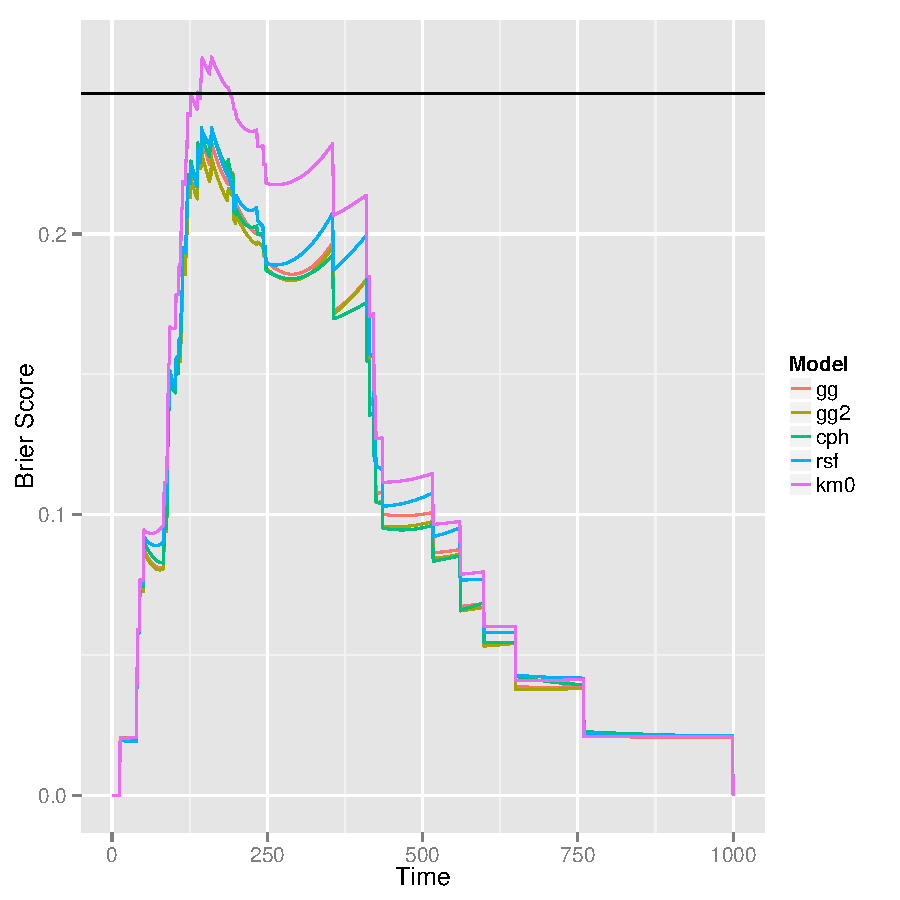
\includegraphics[width=\maxwidth]{figure/model-selection-bs-paths-1} 

}


\begin{kframe}\begin{alltt}
\hlstd{temp} \hlkwb{=} \hlkwd{melt}\hlstd{(}\hlkwd{aaply}\hlstd{(bsc_boots,} \hlnum{2}\hlopt{:}\hlnum{3}\hlstd{, quantile,} \hlkwc{probs} \hlstd{=} \hlkwd{c}\hlstd{(}\hlnum{0.05}\hlstd{,} \hlnum{0.5}\hlstd{,} \hlnum{0.95}\hlstd{)))}
\hlkwd{colnames}\hlstd{(temp)} \hlkwb{=} \hlkwd{c}\hlstd{(}\hlstr{"Model"}\hlstd{,} \hlstr{"Time"}\hlstd{,} \hlstr{"Quantile"}\hlstd{,} \hlstr{"Value"}\hlstd{)}
\hlstd{temp}\hlopt{$}\hlstd{Quantile} \hlkwb{=} \hlkwd{paste}\hlstd{(}\hlstr{"Q"}\hlstd{,} \hlkwd{gsub}\hlstd{(}\hlstr{"%"}\hlstd{,} \hlstr{""}\hlstd{, temp}\hlopt{$}\hlstd{Quantile),} \hlkwc{sep} \hlstd{=} \hlstr{""}\hlstd{)}
\hlstd{temp} \hlkwb{=} \hlkwd{dcast}\hlstd{(temp, Model} \hlopt{+} \hlstd{Time} \hlopt{~} \hlstd{Quantile,} \hlkwc{value.var} \hlstd{=} \hlstr{"Value"}\hlstd{)}
\hlkwd{ggplot}\hlstd{(temp,} \hlkwd{aes}\hlstd{(}\hlkwc{x} \hlstd{= Time,} \hlkwc{y} \hlstd{= Q50,} \hlkwc{ymin} \hlstd{= Q5,} \hlkwc{ymax} \hlstd{= Q95,} \hlkwc{colour} \hlstd{= Model,} \hlkwc{fill} \hlstd{= Model))} \hlopt{+}
    \hlkwd{geom_line}\hlstd{()} \hlopt{+} \hlkwd{geom_ribbon}\hlstd{(}\hlkwc{alpha} \hlstd{=} \hlnum{0.2}\hlstd{,} \hlkwc{colour} \hlstd{=} \hlnum{NA}\hlstd{)} \hlopt{+} \hlkwd{ylab}\hlstd{(}\hlstr{"Brier Score, 90% BI"}\hlstd{)} \hlopt{+}
    \hlkwd{geom_hline}\hlstd{(}\hlkwc{yintercept} \hlstd{=} \hlnum{0.25}\hlstd{)}
\end{alltt}
\end{kframe}

{\centering 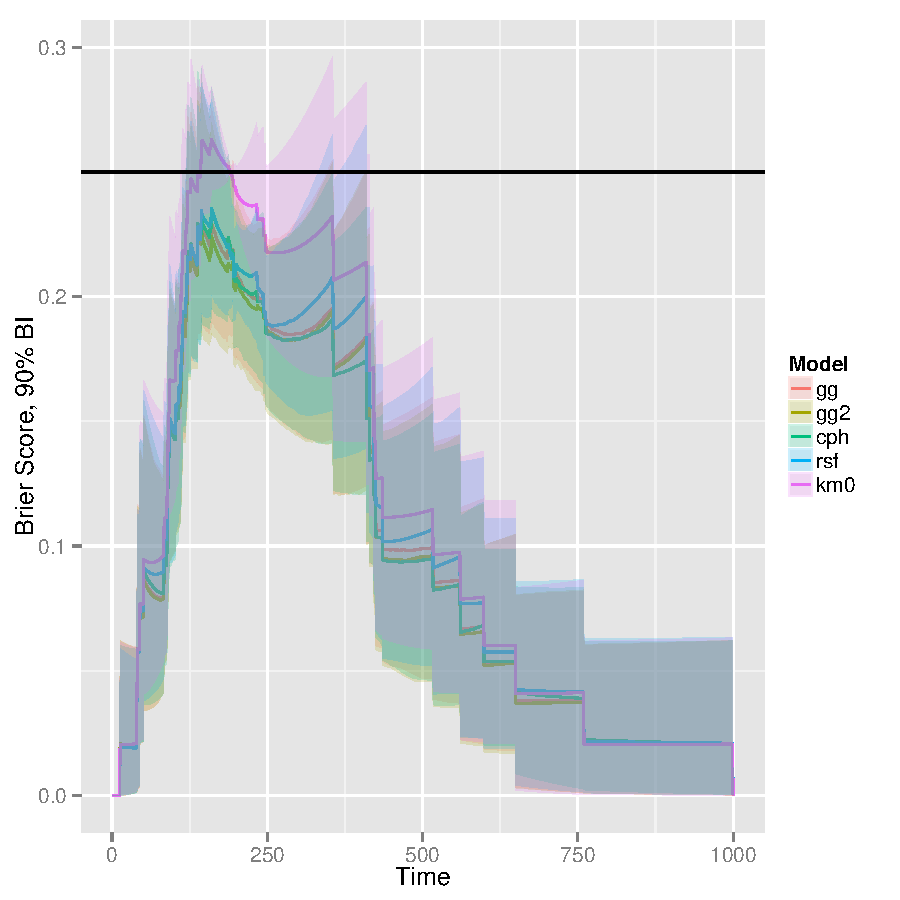
\includegraphics[width=\maxwidth]{figure/model-selection-bs-paths-2} 

}


\begin{kframe}\begin{alltt}
\hlstd{bsc_boots_diff} \hlkwb{=} \hlkwd{aaply}\hlstd{(bsc_boots,} \hlnum{2}\hlstd{,} \hlkwa{function}\hlstd{(}\hlkwc{x}\hlstd{) x} \hlopt{-} \hlstd{bsc_boots[,} \hlnum{5}\hlstd{, ])[}\hlnum{1}\hlopt{:}\hlnum{4}\hlstd{,}
    \hlstd{, ]}
\hlstd{temp} \hlkwb{=} \hlkwd{melt}\hlstd{(}\hlkwd{aaply}\hlstd{(bsc_boots_diff,} \hlkwd{c}\hlstd{(}\hlnum{1}\hlstd{,} \hlnum{3}\hlstd{), quantile,} \hlkwc{probs} \hlstd{=} \hlkwd{c}\hlstd{(}\hlnum{0.05}\hlstd{,} \hlnum{0.5}\hlstd{,} \hlnum{0.95}\hlstd{)))}
\hlkwd{colnames}\hlstd{(temp)} \hlkwb{=} \hlkwd{c}\hlstd{(}\hlstr{"Model"}\hlstd{,} \hlstr{"Time"}\hlstd{,} \hlstr{"Quantile"}\hlstd{,} \hlstr{"Value"}\hlstd{)}
\hlstd{temp}\hlopt{$}\hlstd{Quantile} \hlkwb{=} \hlkwd{paste}\hlstd{(}\hlstr{"Q"}\hlstd{,} \hlkwd{gsub}\hlstd{(}\hlstr{"%"}\hlstd{,} \hlstr{""}\hlstd{, temp}\hlopt{$}\hlstd{Quantile),} \hlkwc{sep} \hlstd{=} \hlstr{""}\hlstd{)}
\hlstd{temp} \hlkwb{=} \hlkwd{dcast}\hlstd{(temp, Model} \hlopt{+} \hlstd{Time} \hlopt{~} \hlstd{Quantile,} \hlkwc{value.var} \hlstd{=} \hlstr{"Value"}\hlstd{)}
\hlkwd{ggplot}\hlstd{(temp,} \hlkwd{aes}\hlstd{(}\hlkwc{x} \hlstd{= Time,} \hlkwc{y} \hlstd{= Q50,} \hlkwc{ymin} \hlstd{= Q5,} \hlkwc{ymax} \hlstd{= Q95,} \hlkwc{colour} \hlstd{= Model,} \hlkwc{fill} \hlstd{= Model))} \hlopt{+}
    \hlkwd{geom_line}\hlstd{()} \hlopt{+} \hlkwd{geom_ribbon}\hlstd{(}\hlkwc{alpha} \hlstd{=} \hlnum{0.2}\hlstd{,} \hlkwc{colour} \hlstd{=} \hlnum{NA}\hlstd{)} \hlopt{+} \hlkwd{ylab}\hlstd{(}\hlstr{"Brier Score: Improvement over KM0. BS median, 90% BI"}\hlstd{)} \hlopt{+}
    \hlkwd{geom_hline}\hlstd{(}\hlkwc{yintercept} \hlstd{=} \hlnum{0}\hlstd{)}
\end{alltt}
\end{kframe}

{\centering 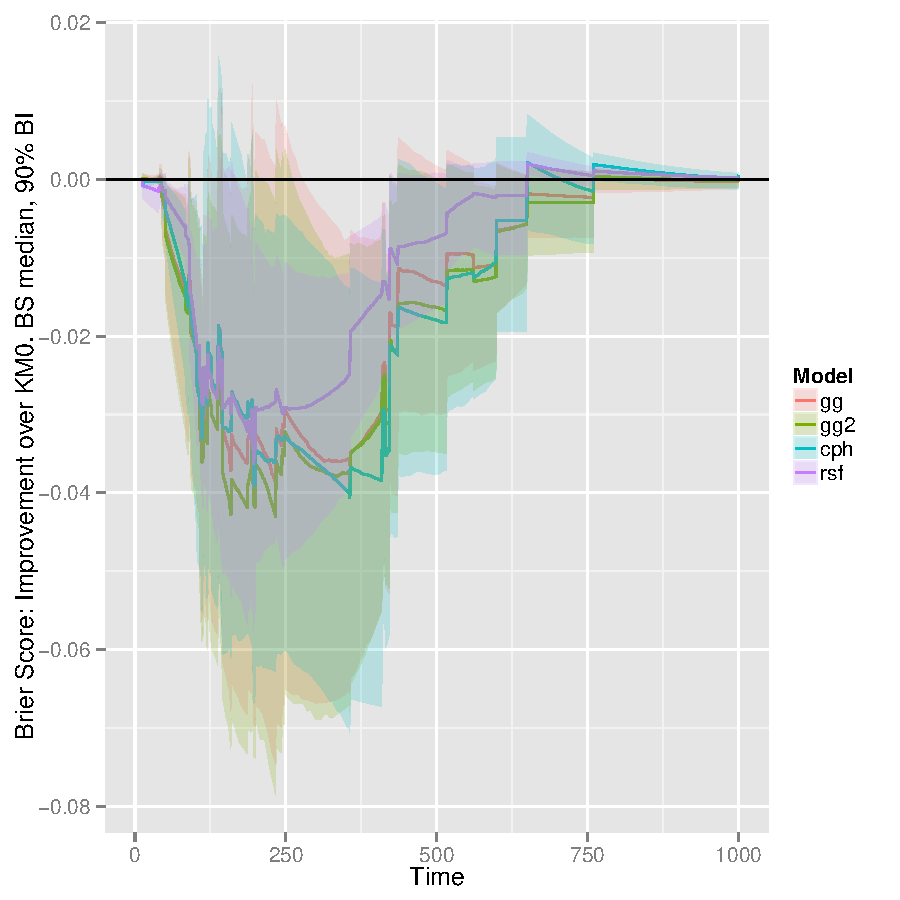
\includegraphics[width=\maxwidth]{figure/model-selection-bs-paths-3} 

}


\begin{kframe}\begin{alltt}
\hlkwd{ggplot}\hlstd{(temp,} \hlkwd{aes}\hlstd{(}\hlkwc{x} \hlstd{= Time,} \hlkwc{y} \hlstd{= Q50,} \hlkwc{ymin} \hlstd{= Q5,} \hlkwc{ymax} \hlstd{= Q95,} \hlkwc{colour} \hlstd{= Model,} \hlkwc{fill} \hlstd{= Model))} \hlopt{+}
    \hlkwd{geom_line}\hlstd{()} \hlopt{+} \hlkwd{geom_ribbon}\hlstd{(}\hlkwc{alpha} \hlstd{=} \hlnum{0.2}\hlstd{,} \hlkwc{colour} \hlstd{=} \hlnum{NA}\hlstd{)} \hlopt{+} \hlkwd{xlim}\hlstd{(}\hlnum{0}\hlstd{,} \hlnum{700}\hlstd{)} \hlopt{+} \hlkwd{ylab}\hlstd{(}\hlstr{"Brier Score: Improvement over KM0. BS median, 90% BI"}\hlstd{)} \hlopt{+}
    \hlkwd{geom_hline}\hlstd{(}\hlkwc{yintercept} \hlstd{=} \hlnum{0}\hlstd{)}
\end{alltt}


{\ttfamily\noindent\color{warningcolor}{\#\# Warning: Removed 1200 rows containing missing values (geom\_path).}}\end{kframe}

{\centering 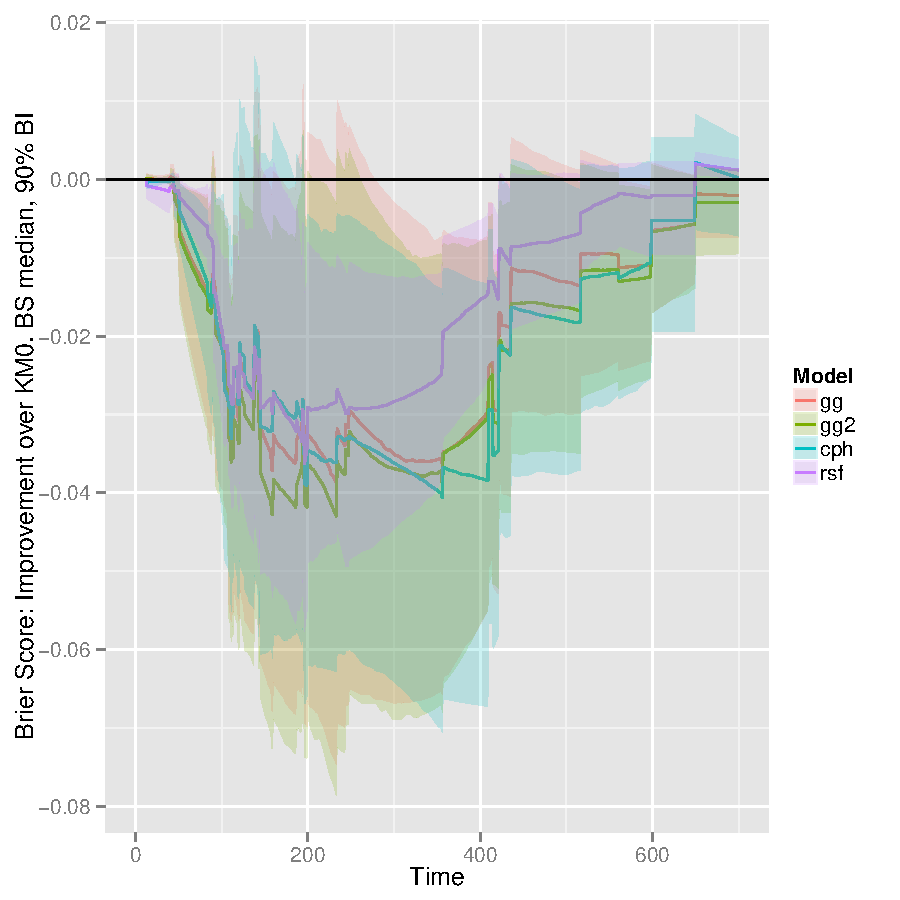
\includegraphics[width=\maxwidth]{figure/model-selection-bs-paths-4} 

}


\begin{kframe}\begin{alltt}
\hlkwd{ggplot}\hlstd{(temp,} \hlkwd{aes}\hlstd{(}\hlkwc{x} \hlstd{= Time,} \hlkwc{y} \hlstd{= Q50,} \hlkwc{colour} \hlstd{= Model))} \hlopt{+} \hlkwd{geom_line}\hlstd{()} \hlopt{+} \hlkwd{ylab}\hlstd{(}\hlstr{"Brier Score: Improvement over KM0, BS median"}\hlstd{)} \hlopt{+}
    \hlkwd{geom_hline}\hlstd{(}\hlkwc{yintercept} \hlstd{=} \hlnum{0}\hlstd{)}
\end{alltt}
\end{kframe}

{\centering 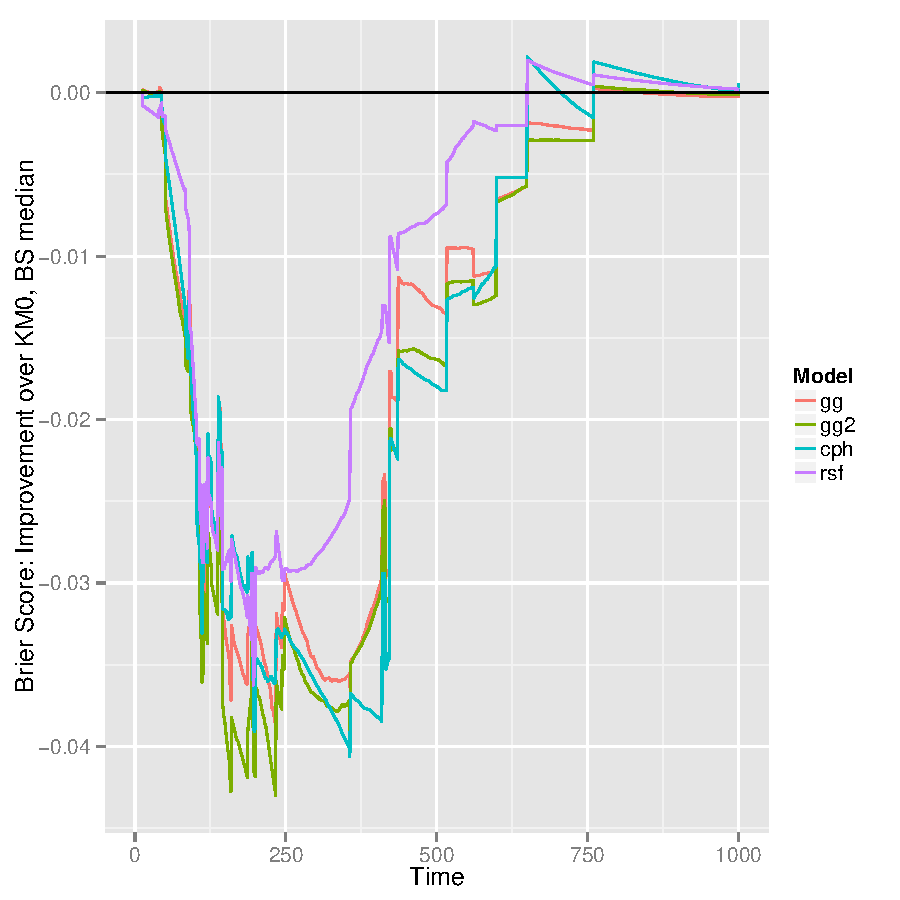
\includegraphics[width=\maxwidth]{figure/model-selection-bs-paths-5} 

}


\begin{kframe}\begin{alltt}
\hlkwd{ggplot}\hlstd{(temp,} \hlkwd{aes}\hlstd{(}\hlkwc{x} \hlstd{= Time,} \hlkwc{y} \hlstd{= Q50,} \hlkwc{colour} \hlstd{= Model))} \hlopt{+} \hlkwd{geom_line}\hlstd{()} \hlopt{+} \hlkwd{ylab}\hlstd{(}\hlstr{"Brier Score: Improvement over KM0, BS median"}\hlstd{)} \hlopt{+}
    \hlkwd{xlim}\hlstd{(}\hlnum{0}\hlstd{,} \hlnum{700}\hlstd{)} \hlopt{+} \hlkwd{geom_hline}\hlstd{(}\hlkwc{yintercept} \hlstd{=} \hlnum{0}\hlstd{)}
\end{alltt}


{\ttfamily\noindent\color{warningcolor}{\#\# Warning: Removed 1200 rows containing missing values (geom\_path).}}\end{kframe}

{\centering 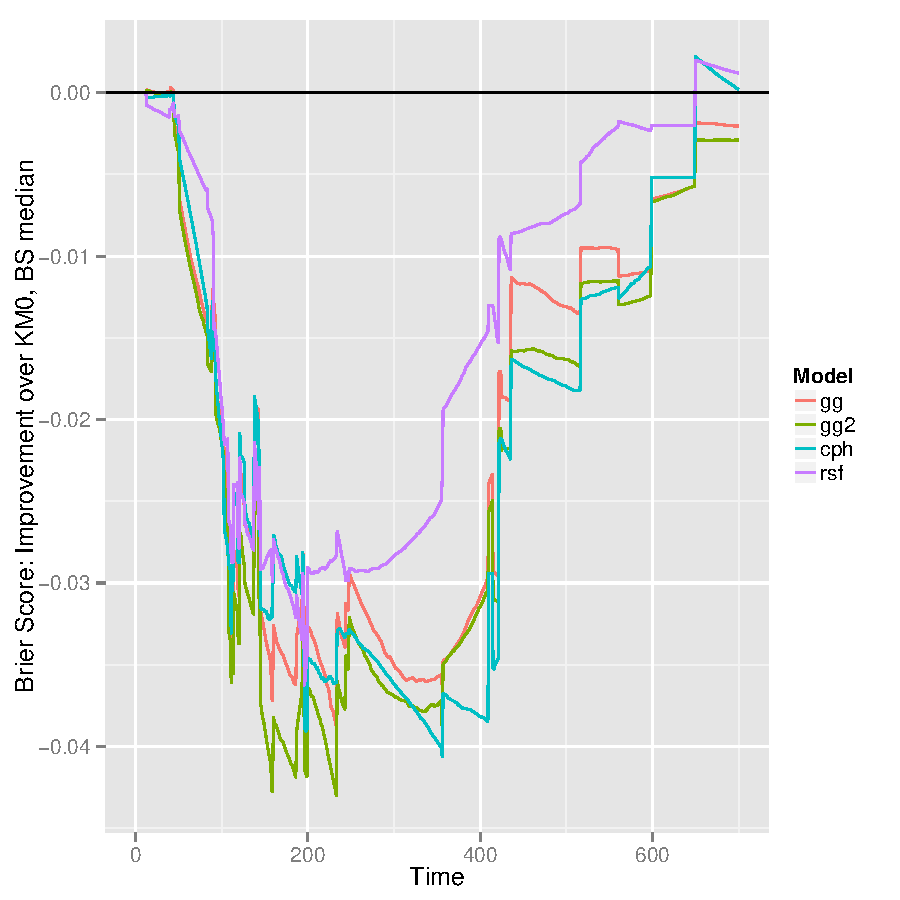
\includegraphics[width=\maxwidth]{figure/model-selection-bs-paths-6} 

}



\end{knitrout}

IBS comparisons.
\begin{knitrout}
\definecolor{shadecolor}{rgb}{0.969, 0.969, 0.969}\color{fgcolor}\begin{kframe}
\begin{alltt}
\hlkwd{set.seed}\hlstd{(}\hlnum{20150111}\hlstd{)}
\hlstd{ibsc_boots} \hlkwb{=} \hlkwd{t}\hlstd{(}\hlkwd{sapply}\hlstd{(}\hlnum{1}\hlopt{:}\hlnum{500}\hlstd{,} \hlkwa{function}\hlstd{(}\hlkwc{i}\hlstd{) \{}
    \hlkwa{if} \hlstd{(i}\hlopt\hlnum{50} \hlopt{==} \hlnum{0}\hlstd{) \{}
        \hlkwd{message}\hlstd{(i)}
    \hlstd{\}}
    \hlstd{boot_samp} \hlkwb{=} \hlkwd{sample.int}\hlstd{(}\hlkwd{nrow}\hlstd{(data.val),} \hlkwc{replace} \hlstd{=} \hlnum{TRUE}\hlstd{)}
    \hlstd{gg} \hlkwb{=} \hlkwd{calcIBS}\hlstd{(}\hlkwd{Surv}\hlstd{(data.val}\hlopt{$}\hlstd{Time, data.val}\hlopt{$}\hlstd{DSD)[boot_samp, ], ibs_preds_gg[boot_samp,}
        \hlstd{], ibs_times,} \hlkwd{max}\hlstd{(data.val}\hlopt{$}\hlstd{Time[boot_samp]))}\hlopt{$}\hlstd{ibs}
    \hlstd{gg2} \hlkwb{=} \hlkwd{calcIBS}\hlstd{(}\hlkwd{Surv}\hlstd{(data.val}\hlopt{$}\hlstd{Time, data.val}\hlopt{$}\hlstd{DSD)[boot_samp, ], ibs_preds_gg2[boot_samp,}
        \hlstd{], ibs_times,} \hlkwd{max}\hlstd{(data.val}\hlopt{$}\hlstd{Time[boot_samp]))}\hlopt{$}\hlstd{ibs}
    \hlstd{cph} \hlkwb{=} \hlkwd{calcIBS}\hlstd{(}\hlkwd{Surv}\hlstd{(data.val}\hlopt{$}\hlstd{Time, data.val}\hlopt{$}\hlstd{DSD)[boot_samp, ], ibs_preds_cph[boot_samp,}
        \hlstd{], ibs_times,} \hlkwd{max}\hlstd{(data.val}\hlopt{$}\hlstd{Time[boot_samp]))}\hlopt{$}\hlstd{ibs}
    \hlstd{rsf} \hlkwb{=} \hlkwd{calcIBS}\hlstd{(}\hlkwd{Surv}\hlstd{(data.val}\hlopt{$}\hlstd{Time, data.val}\hlopt{$}\hlstd{DSD)[boot_samp, ], ibs_preds_rsf[boot_samp,}
        \hlstd{], ibs_times,} \hlkwd{max}\hlstd{(data.val}\hlopt{$}\hlstd{Time[boot_samp]))}\hlopt{$}\hlstd{ibs}
    \hlstd{km0} \hlkwb{=} \hlkwd{calcIBS}\hlstd{(}\hlkwd{Surv}\hlstd{(data.val}\hlopt{$}\hlstd{Time, data.val}\hlopt{$}\hlstd{DSD)[boot_samp, ], ibs_preds_km0[boot_samp,}
        \hlstd{], ibs_times,} \hlkwd{max}\hlstd{(data.val}\hlopt{$}\hlstd{Time[boot_samp]))}\hlopt{$}\hlstd{ibs}
    \hlkwd{c}\hlstd{(gg, gg2, cph, rsf, km0)}
\hlstd{\}))}
\end{alltt}


{\ttfamily\noindent\itshape\color{messagecolor}{\#\# 50\\\#\# 100\\\#\# 150\\\#\# 200\\\#\# 250\\\#\# 300\\\#\# 350\\\#\# 400\\\#\# 450\\\#\# 500}}\begin{alltt}
\hlkwd{colnames}\hlstd{(ibsc_boots)} \hlkwb{=} \hlkwd{c}\hlstd{(}\hlstr{"gg"}\hlstd{,} \hlstr{"gg2"}\hlstd{,} \hlstr{"cph"}\hlstd{,} \hlstr{"rsf"}\hlstd{,} \hlstr{"km0"}\hlstd{)}
\end{alltt}
\end{kframe}
\end{knitrout}

\begin{knitrout}
\definecolor{shadecolor}{rgb}{0.969, 0.969, 0.969}\color{fgcolor}\begin{kframe}
\begin{alltt}
\hlkwd{calcIBS}\hlstd{(}\hlkwd{Surv}\hlstd{(data.val}\hlopt{$}\hlstd{Time, data.val}\hlopt{$}\hlstd{DSD), ibs_preds_gg, ibs_times,} \hlkwd{max}\hlstd{(data.val}\hlopt{$}\hlstd{Time))}\hlopt{$}\hlstd{ibs}
\end{alltt}
\begin{verbatim}
## [1] 162.1
\end{verbatim}
\begin{alltt}
\hlkwd{calcIBS}\hlstd{(}\hlkwd{Surv}\hlstd{(data.val}\hlopt{$}\hlstd{Time, data.val}\hlopt{$}\hlstd{DSD), ibs_preds_gg2, ibs_times,} \hlkwd{max}\hlstd{(data.val}\hlopt{$}\hlstd{Time))}\hlopt{$}\hlstd{ibs}
\end{alltt}
\begin{verbatim}
## [1] 159.5
\end{verbatim}
\begin{alltt}
\hlkwd{calcIBS}\hlstd{(}\hlkwd{Surv}\hlstd{(data.val}\hlopt{$}\hlstd{Time, data.val}\hlopt{$}\hlstd{DSD), ibs_preds_cph, ibs_times,} \hlkwd{max}\hlstd{(data.val}\hlopt{$}\hlstd{Time))}\hlopt{$}\hlstd{ibs}
\end{alltt}
\begin{verbatim}
## [1] 161.2
\end{verbatim}
\begin{alltt}
\hlkwd{calcIBS}\hlstd{(}\hlkwd{Surv}\hlstd{(data.val}\hlopt{$}\hlstd{Time, data.val}\hlopt{$}\hlstd{DSD), ibs_preds_rsf, ibs_times,} \hlkwd{max}\hlstd{(data.val}\hlopt{$}\hlstd{Time))}\hlopt{$}\hlstd{ibs}
\end{alltt}
\begin{verbatim}
## [1] 170.1
\end{verbatim}
\begin{alltt}
\hlkwd{calcIBS}\hlstd{(}\hlkwd{Surv}\hlstd{(data.val}\hlopt{$}\hlstd{Time, data.val}\hlopt{$}\hlstd{DSD), ibs_preds_km0, ibs_times,} \hlkwd{max}\hlstd{(data.val}\hlopt{$}\hlstd{Time))}\hlopt{$}\hlstd{ibs}
\end{alltt}
\begin{verbatim}
## [1] 184.4
\end{verbatim}
\begin{alltt}
\hlkwd{boxplot}\hlstd{(ibsc_boots,} \hlkwc{main} \hlstd{=} \hlstr{"IBS BS Distribution"}\hlstd{,} \hlkwc{ylab} \hlstd{=} \hlstr{"IBS"}\hlstd{)}
\end{alltt}
\end{kframe}

{\centering 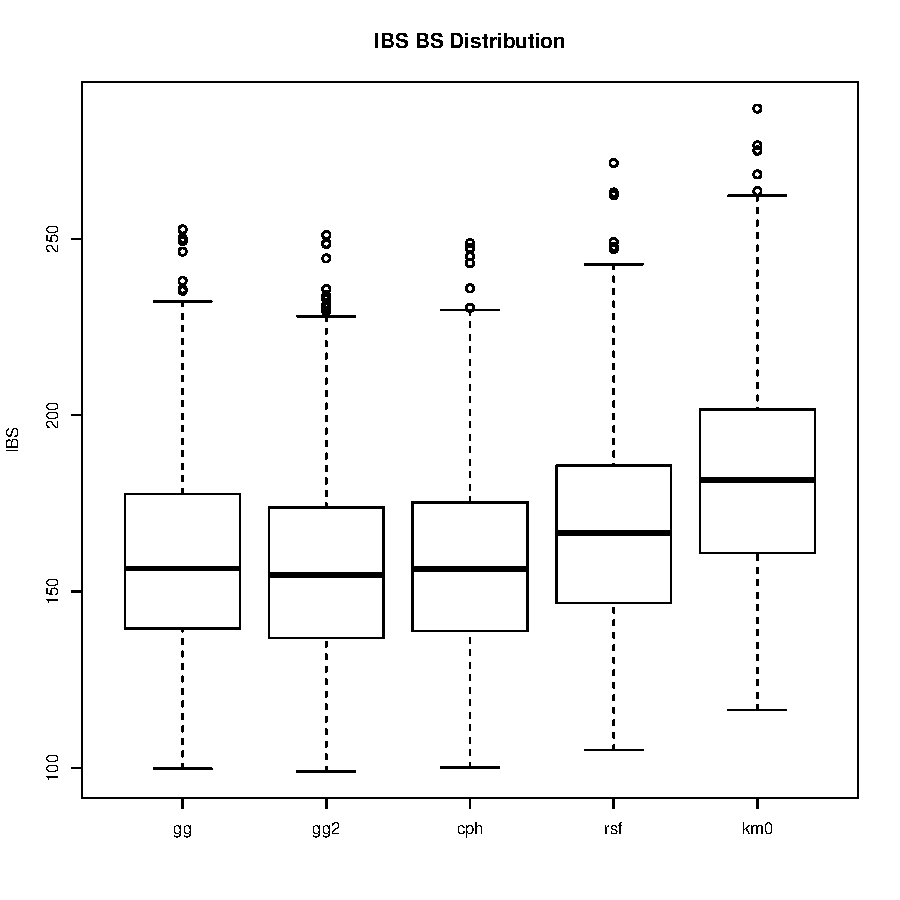
\includegraphics[width=\maxwidth]{figure/model-selection-ibs-1} 

}


\begin{kframe}\begin{alltt}
\hlkwd{plot}\hlstd{(}\hlkwd{density}\hlstd{(ibsc_boots[,} \hlnum{1}\hlstd{]),} \hlkwc{col} \hlstd{=} \hlstr{"blue"}\hlstd{,} \hlkwc{lwd} \hlstd{=} \hlnum{2}\hlstd{,} \hlkwc{main} \hlstd{=} \hlstr{"IBS BS Distribution"}\hlstd{,}
    \hlkwc{xlab} \hlstd{=} \hlstr{"IBS"}\hlstd{)}
\hlkwd{lines}\hlstd{(}\hlkwd{density}\hlstd{(ibsc_boots[,} \hlnum{2}\hlstd{]),} \hlkwc{col} \hlstd{=} \hlstr{"red"}\hlstd{,} \hlkwc{lwd} \hlstd{=} \hlnum{2}\hlstd{)}
\hlkwd{lines}\hlstd{(}\hlkwd{density}\hlstd{(ibsc_boots[,} \hlnum{3}\hlstd{]),} \hlkwc{col} \hlstd{=} \hlstr{"green"}\hlstd{,} \hlkwc{lwd} \hlstd{=} \hlnum{2}\hlstd{)}
\hlkwd{lines}\hlstd{(}\hlkwd{density}\hlstd{(ibsc_boots[,} \hlnum{4}\hlstd{]),} \hlkwc{col} \hlstd{=} \hlstr{"purple"}\hlstd{,} \hlkwc{lwd} \hlstd{=} \hlnum{2}\hlstd{)}
\hlkwd{lines}\hlstd{(}\hlkwd{density}\hlstd{(ibsc_boots[,} \hlnum{5}\hlstd{]),} \hlkwc{col} \hlstd{=} \hlstr{"black"}\hlstd{,} \hlkwc{lwd} \hlstd{=} \hlnum{2}\hlstd{)}
\hlkwd{abline}\hlstd{(}\hlkwc{v} \hlstd{=} \hlkwd{calcIBS}\hlstd{(}\hlkwd{Surv}\hlstd{(data.val}\hlopt{$}\hlstd{Time, data.val}\hlopt{$}\hlstd{DSD), ibs_preds_gg, ibs_times,}
    \hlkwd{max}\hlstd{(data.val}\hlopt{$}\hlstd{Time))}\hlopt{$}\hlstd{ibs,} \hlkwc{col} \hlstd{=} \hlstr{"blue"}\hlstd{,} \hlkwc{lwd} \hlstd{=} \hlnum{1}\hlstd{)}
\hlkwd{abline}\hlstd{(}\hlkwc{v} \hlstd{=} \hlkwd{calcIBS}\hlstd{(}\hlkwd{Surv}\hlstd{(data.val}\hlopt{$}\hlstd{Time, data.val}\hlopt{$}\hlstd{DSD), ibs_preds_gg2, ibs_times,}
    \hlkwd{max}\hlstd{(data.val}\hlopt{$}\hlstd{Time))}\hlopt{$}\hlstd{ibs,} \hlkwc{col} \hlstd{=} \hlstr{"red"}\hlstd{,} \hlkwc{lwd} \hlstd{=} \hlnum{1}\hlstd{)}
\hlkwd{abline}\hlstd{(}\hlkwc{v} \hlstd{=} \hlkwd{calcIBS}\hlstd{(}\hlkwd{Surv}\hlstd{(data.val}\hlopt{$}\hlstd{Time, data.val}\hlopt{$}\hlstd{DSD), ibs_preds_cph, ibs_times,}
    \hlkwd{max}\hlstd{(data.val}\hlopt{$}\hlstd{Time))}\hlopt{$}\hlstd{ibs,} \hlkwc{col} \hlstd{=} \hlstr{"green"}\hlstd{,} \hlkwc{lwd} \hlstd{=} \hlnum{1}\hlstd{)}
\hlkwd{abline}\hlstd{(}\hlkwc{v} \hlstd{=} \hlkwd{calcIBS}\hlstd{(}\hlkwd{Surv}\hlstd{(data.val}\hlopt{$}\hlstd{Time, data.val}\hlopt{$}\hlstd{DSD), ibs_preds_rsf, ibs_times,}
    \hlkwd{max}\hlstd{(data.val}\hlopt{$}\hlstd{Time))}\hlopt{$}\hlstd{ibs,} \hlkwc{col} \hlstd{=} \hlstr{"purple"}\hlstd{,} \hlkwc{lwd} \hlstd{=} \hlnum{1}\hlstd{)}
\hlkwd{abline}\hlstd{(}\hlkwc{v} \hlstd{=} \hlkwd{calcIBS}\hlstd{(}\hlkwd{Surv}\hlstd{(data.val}\hlopt{$}\hlstd{Time, data.val}\hlopt{$}\hlstd{DSD), ibs_preds_km0, ibs_times,}
    \hlkwd{max}\hlstd{(data.val}\hlopt{$}\hlstd{Time))}\hlopt{$}\hlstd{ibs,} \hlkwc{col} \hlstd{=} \hlstr{"black"}\hlstd{,} \hlkwc{lwd} \hlstd{=} \hlnum{1}\hlstd{)}
\hlkwd{legend}\hlstd{(}\hlstr{"topright"}\hlstd{,} \hlkwc{legend} \hlstd{=} \hlkwd{c}\hlstd{(}\hlstr{"gg"}\hlstd{,} \hlstr{"gg2"}\hlstd{,} \hlstr{"cph"}\hlstd{,} \hlstr{"rsf"}\hlstd{,} \hlstr{"km0"}\hlstd{),} \hlkwc{col} \hlstd{=} \hlkwd{c}\hlstd{(}\hlstr{"blue"}\hlstd{,}
    \hlstr{"red"}\hlstd{,} \hlstr{"green"}\hlstd{,} \hlstr{"purple"}\hlstd{,} \hlstr{"black"}\hlstd{),} \hlkwc{lty} \hlstd{=} \hlstr{"solid"}\hlstd{,} \hlkwc{inset} \hlstd{=} \hlnum{0.05}\hlstd{)}
\end{alltt}
\end{kframe}

{\centering 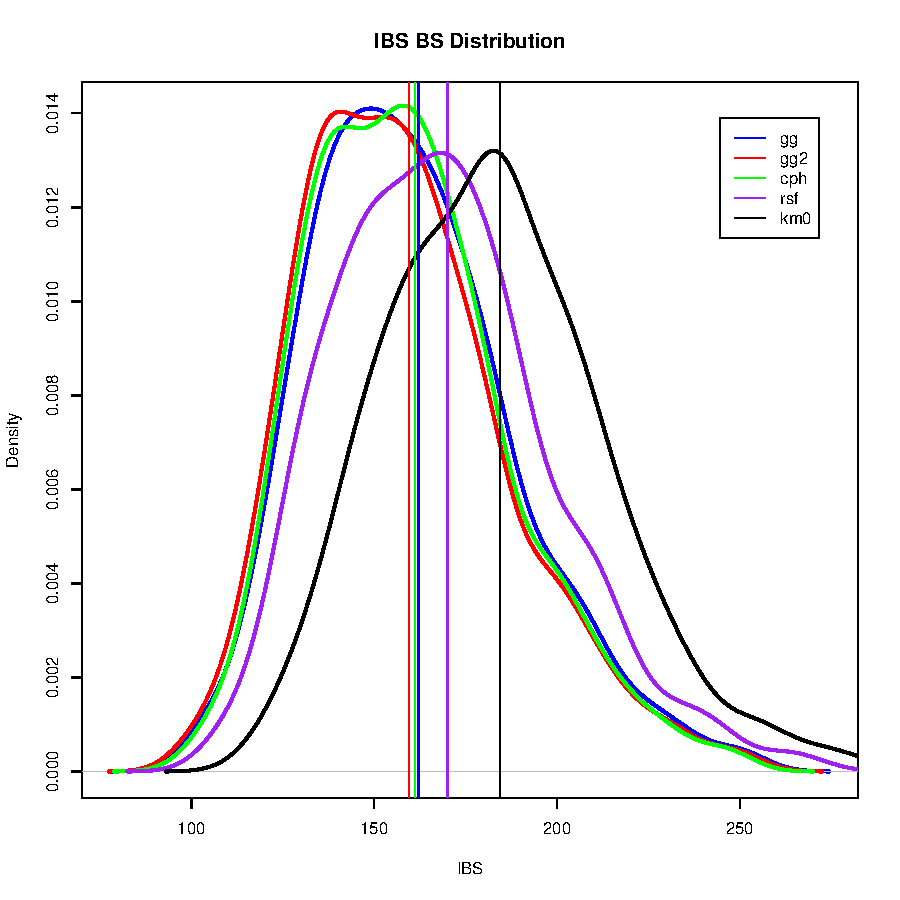
\includegraphics[width=\maxwidth]{figure/model-selection-ibs-2} 

}


\begin{kframe}\begin{alltt}
\hlkwd{plot}\hlstd{(}\hlkwd{density}\hlstd{(ibsc_boots[,} \hlnum{5}\hlstd{]} \hlopt{-} \hlstd{ibsc_boots[,} \hlnum{1}\hlstd{]),} \hlkwc{col} \hlstd{=} \hlstr{"blue"}\hlstd{,} \hlkwc{lwd} \hlstd{=} \hlnum{2}\hlstd{,} \hlkwc{main} \hlstd{=} \hlstr{"IBS_x - IBS_KM0 BS Distribution"}\hlstd{,}
    \hlkwc{xlab} \hlstd{=} \hlstr{"IBS"}\hlstd{,} \hlkwc{ylim} \hlstd{=} \hlkwd{c}\hlstd{(}\hlnum{0}\hlstd{,} \hlnum{0.1}\hlstd{))}
\hlkwd{lines}\hlstd{(}\hlkwd{density}\hlstd{(ibsc_boots[,} \hlnum{5}\hlstd{]} \hlopt{-} \hlstd{ibsc_boots[,} \hlnum{2}\hlstd{]),} \hlkwc{col} \hlstd{=} \hlstr{"red"}\hlstd{,} \hlkwc{lwd} \hlstd{=} \hlnum{2}\hlstd{)}
\hlkwd{lines}\hlstd{(}\hlkwd{density}\hlstd{(ibsc_boots[,} \hlnum{5}\hlstd{]} \hlopt{-} \hlstd{ibsc_boots[,} \hlnum{3}\hlstd{]),} \hlkwc{col} \hlstd{=} \hlstr{"green"}\hlstd{,} \hlkwc{lwd} \hlstd{=} \hlnum{2}\hlstd{)}
\hlkwd{lines}\hlstd{(}\hlkwd{density}\hlstd{(ibsc_boots[,} \hlnum{5}\hlstd{]} \hlopt{-} \hlstd{ibsc_boots[,} \hlnum{4}\hlstd{]),} \hlkwc{col} \hlstd{=} \hlstr{"purple"}\hlstd{,} \hlkwc{lwd} \hlstd{=} \hlnum{2}\hlstd{)}
\hlkwd{abline}\hlstd{(}\hlkwc{v} \hlstd{= (}\hlkwd{calcIBS}\hlstd{(}\hlkwd{Surv}\hlstd{(data.val}\hlopt{$}\hlstd{Time, data.val}\hlopt{$}\hlstd{DSD), ibs_preds_km0, ibs_times,}
    \hlkwd{max}\hlstd{(data.val}\hlopt{$}\hlstd{Time))}\hlopt{$}\hlstd{ibs} \hlopt{-} \hlkwd{calcIBS}\hlstd{(}\hlkwd{Surv}\hlstd{(data.val}\hlopt{$}\hlstd{Time, data.val}\hlopt{$}\hlstd{DSD), ibs_preds_gg,}
    \hlstd{ibs_times,} \hlkwd{max}\hlstd{(data.val}\hlopt{$}\hlstd{Time))}\hlopt{$}\hlstd{ibs),} \hlkwc{col} \hlstd{=} \hlstr{"blue"}\hlstd{,} \hlkwc{lwd} \hlstd{=} \hlnum{1}\hlstd{)}
\hlkwd{abline}\hlstd{(}\hlkwc{v} \hlstd{= (}\hlkwd{calcIBS}\hlstd{(}\hlkwd{Surv}\hlstd{(data.val}\hlopt{$}\hlstd{Time, data.val}\hlopt{$}\hlstd{DSD), ibs_preds_km0, ibs_times,}
    \hlkwd{max}\hlstd{(data.val}\hlopt{$}\hlstd{Time))}\hlopt{$}\hlstd{ibs} \hlopt{-} \hlkwd{calcIBS}\hlstd{(}\hlkwd{Surv}\hlstd{(data.val}\hlopt{$}\hlstd{Time, data.val}\hlopt{$}\hlstd{DSD), ibs_preds_gg2,}
    \hlstd{ibs_times,} \hlkwd{max}\hlstd{(data.val}\hlopt{$}\hlstd{Time))}\hlopt{$}\hlstd{ibs),} \hlkwc{col} \hlstd{=} \hlstr{"red"}\hlstd{,} \hlkwc{lwd} \hlstd{=} \hlnum{1}\hlstd{)}
\hlkwd{abline}\hlstd{(}\hlkwc{v} \hlstd{= (}\hlkwd{calcIBS}\hlstd{(}\hlkwd{Surv}\hlstd{(data.val}\hlopt{$}\hlstd{Time, data.val}\hlopt{$}\hlstd{DSD), ibs_preds_km0, ibs_times,}
    \hlkwd{max}\hlstd{(data.val}\hlopt{$}\hlstd{Time))}\hlopt{$}\hlstd{ibs} \hlopt{-} \hlkwd{calcIBS}\hlstd{(}\hlkwd{Surv}\hlstd{(data.val}\hlopt{$}\hlstd{Time, data.val}\hlopt{$}\hlstd{DSD), ibs_preds_cph,}
    \hlstd{ibs_times,} \hlkwd{max}\hlstd{(data.val}\hlopt{$}\hlstd{Time))}\hlopt{$}\hlstd{ibs),} \hlkwc{col} \hlstd{=} \hlstr{"green"}\hlstd{,} \hlkwc{lwd} \hlstd{=} \hlnum{1}\hlstd{)}
\hlkwd{abline}\hlstd{(}\hlkwc{v} \hlstd{= (}\hlkwd{calcIBS}\hlstd{(}\hlkwd{Surv}\hlstd{(data.val}\hlopt{$}\hlstd{Time, data.val}\hlopt{$}\hlstd{DSD), ibs_preds_km0, ibs_times,}
    \hlkwd{max}\hlstd{(data.val}\hlopt{$}\hlstd{Time))}\hlopt{$}\hlstd{ibs} \hlopt{-} \hlkwd{calcIBS}\hlstd{(}\hlkwd{Surv}\hlstd{(data.val}\hlopt{$}\hlstd{Time, data.val}\hlopt{$}\hlstd{DSD), ibs_preds_rsf,}
    \hlstd{ibs_times,} \hlkwd{max}\hlstd{(data.val}\hlopt{$}\hlstd{Time))}\hlopt{$}\hlstd{ibs),} \hlkwc{col} \hlstd{=} \hlstr{"purple"}\hlstd{,} \hlkwc{lwd} \hlstd{=} \hlnum{1}\hlstd{)}
\hlkwd{legend}\hlstd{(}\hlstr{"topright"}\hlstd{,} \hlkwc{legend} \hlstd{=} \hlkwd{c}\hlstd{(}\hlstr{"gg"}\hlstd{,} \hlstr{"gg2"}\hlstd{,} \hlstr{"cph"}\hlstd{,} \hlstr{"rsf"}\hlstd{),} \hlkwc{col} \hlstd{=} \hlkwd{c}\hlstd{(}\hlstr{"blue"}\hlstd{,} \hlstr{"red"}\hlstd{,}
    \hlstr{"green"}\hlstd{,} \hlstr{"purple"}\hlstd{),} \hlkwc{lty} \hlstd{=} \hlstr{"solid"}\hlstd{,} \hlkwc{inset} \hlstd{=} \hlnum{0.05}\hlstd{)}
\end{alltt}
\end{kframe}

{\centering 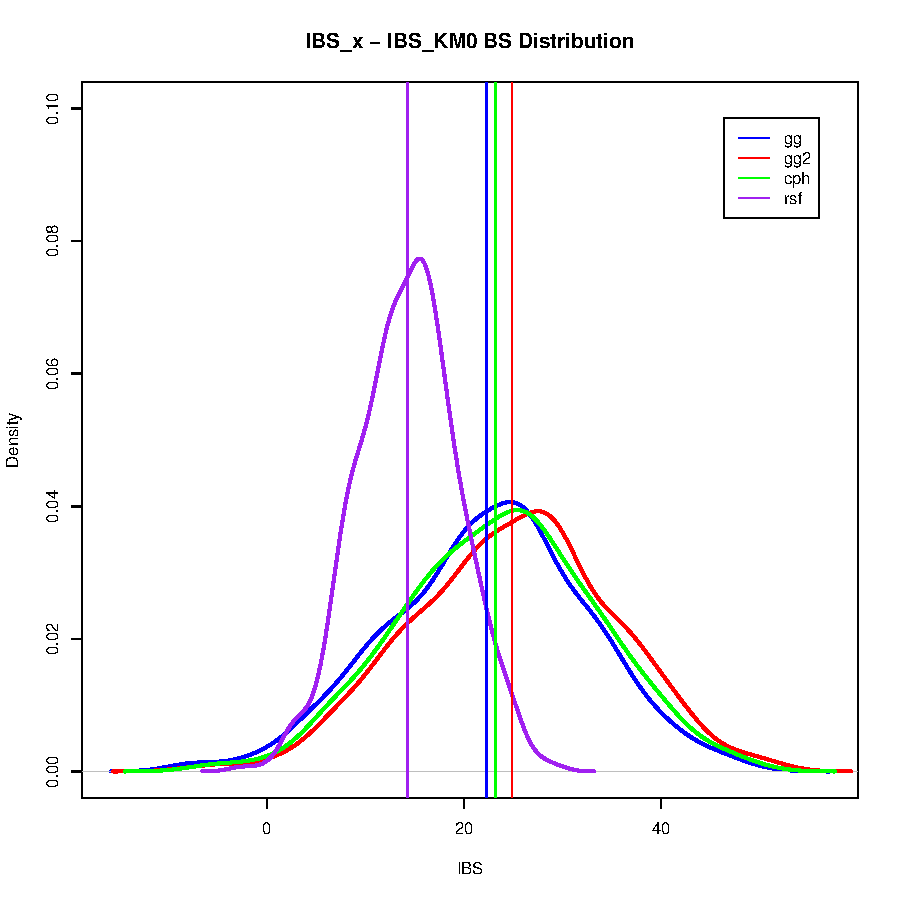
\includegraphics[width=\maxwidth]{figure/model-selection-ibs-3} 

}



\end{knitrout}
All models perform equivalently on the validation set.  Select the simplest: gg.


%%%%%%%%%%%%%%%%%%%%%%%%%%%%%%%%%%%%%%%%%%%%%%%%%%%%%%%%%%%%%%%%%%%%%%
% THE END
%%%%%%%%%%%%%%%%%%%%%%%%%%%%%%%%%%%%%%%%%%%%%%%%%%%%%%%%%%%%%%%%%%%%%%
\section{Session information}
\begin{knitrout}
\definecolor{shadecolor}{rgb}{0.969, 0.969, 0.969}\color{fgcolor}\begin{kframe}
\begin{alltt}
\hlkwd{sessionInfo}\hlstd{()}
\end{alltt}
\begin{verbatim}
## R version 3.1.1 (2014-07-10)
## Platform: x86_64-unknown-linux-gnu (64-bit)
## 
## locale:
##  [1] LC_CTYPE=en_US.UTF-8          LC_NUMERIC=C                 
##  [3] LC_TIME=en_US.UTF-8           LC_COLLATE=en_US.UTF-8       
##  [5] LC_MONETARY=en_US.UTF-8       LC_MESSAGES=en_US.UTF-8      
##  [7] LC_PAPER=en_US.UTF-8          LC_NAME=en_US.UTF-8          
##  [9] LC_ADDRESS=en_US.UTF-8        LC_TELEPHONE=en_US.UTF-8     
## [11] LC_MEASUREMENT=en_US.UTF-8    LC_IDENTIFICATION=en_US.UTF-8
## 
## attached base packages:
## [1] parallel  methods   splines   stats     graphics  grDevices utils    
## [8] datasets  base     
## 
## other attached packages:
##  [1] MASS_7.3-35           ggplot2_1.0.0         plyr_1.8.1           
##  [4] reshape2_1.4          randomForestSRC_1.5.5 flexsurv_0.5         
##  [7] glmulti_1.0.7         rJava_0.9-6           survival_2.37-7      
## [10] knitr_1.8            
## 
## loaded via a namespace (and not attached):
##  [1] codetools_0.2-9  colorspace_1.2-4 deSolve_1.11     digest_0.6.4    
##  [5] evaluate_0.5.5   formatR_1.0      grid_3.1.1       gtable_0.1.2    
##  [9] highr_0.4        labeling_0.3     muhaz_1.2.6      munsell_0.4.2   
## [13] mvtnorm_1.0-1    proto_0.3-10     Rcpp_0.11.3      scales_0.2.4    
## [17] stringr_0.6.2    tools_3.1.1
\end{verbatim}
\end{kframe}
\end{knitrout}

\end{document}



